\documentclass[12pt]{report}
\usepackage{ECE_Dissertation_Style}
\usepackage{amsmath,amssymb,latexsym,float,epsfig,subfigure,overpic}
%these margins allow you to use the default "shrink oversize pages" option when printing
\usepackage[lmargin=1.40 in, rmargin=0.86 in,tmargin=1.0 in,bmargin=1.0 in]{geometry}
\usepackage{indentfirst}
\usepackage{afterpage}
\usepackage{sectsty}
\usepackage{hyperref}
\usepackage{caption}
\usepackage{etoolbox}
\usepackage[per-mode=symbol, detect-weight=true, binary-units=true]{siunitx}
\DeclareSIUnit \amperehour{ Ah }
%%% bookmarks - color them black
\hypersetup{
	colorlinks=true,
	citecolor=black,
	filecolor=black,
	linkcolor=black,
	urlcolor=black
}
%Set graphics path
\graphicspath{{./pictures/},{./pictures/pdf/},{./pictures/ps/},{./pictures/png/},{./pictures/jpg/}}
\captionsetup{format=hang}
%Fill pages with text and floats
\renewcommand\textfraction{.1}
\renewcommand\topfraction{.9}
\renewcommand\bottomfraction{.7}
\renewcommand\floatpagefraction{.7}
%Remove white space above chapter headings
\makeatletter
\patchcmd{\@makechapterhead}{\vspace*{50\p@}}{}{}{}% Removes space above \chapter head
\patchcmd{\@makeschapterhead}{\vspace*{50\p@}}{}{}{}% Removes space above \chapter* head
\makeatother

%figures restructuring
\newcommand{\figwid}{0.48\columnwidth}


\begin{document}

%Set limits on font sizes for headings
\chapternumberfont{\fontsize{16}{20}\selectfont}
\chaptertitlefont{\centering\fontsize{16}{20}\selectfont}
\sectionfont{\fontsize{14}{16}\selectfont}
\subsectionfont{\fontsize{12}{14}\selectfont}

%%
%%
\title{Applications of Unmanned Vehicles with Wireless Sensor Networks and Surveying} %% If you want to specify a linebreak
                               %% in the thesis title, you MUST use
                               %% \protect\\ instead of \\, as \\ is a
                               %% fragile command that \MakeUpperCase
                               %% will break!
\author{An Nguyen}
\department{Department of Electrical and Computer Engineering}

%% Can have up to four readers in addition to the advisor.
%% All have the form
%%
%%  \reader{Name}[Department][Institution]
%%
%% The second and third arguments are optional, but if you wish to
%% supply the third, you must supply the second. Department defaults
%% to the department defined above and Institution defaults to a blank.

\advisor{Aaron T. Becker, Assistant Professor}[Department of Electrical Engineering]
\firstreader{Matthew Franchek, Professor}[Department of Mechanical Engineering]
\secondreader{Miao Pan, Assistant Professor}[Department of Electrical Engineering]
%\setcounter{secnumdepth}{2}
\degree{Master of Science}
\major{Electrical Engineering} 

\copyrighttrue
\copyrightyear{2018}
\submitdate{August 2018} % Must be the month and year of graduation,
                         % not thesis approval! As of 2010, this means
                         % this text must be May, August, or December
                         % followed by the year.

%defaults to thesis option
\dissertationfalse

%%%%%%%%%%%%%%%%%%%%%%%%%%%%%%%%%%%%%%%%%%%%%%%%%%%%%%%%%%%%%%%%%%%%%%%%%%%%%%%
% COVER PAGES:  Flyleaf, copyright page, title page, signature page
%
\makecoverpages

%%%%%%%%%%%%%%%%%%%%%%%%%%%%%%%%%%%%%%%%%%%%%%%%%%%%%%%%%%%%%%%%%%%%%%%%%%%%%%%
% ACKNOWLEDGMENTS
%
% Put acknowledgments in a file called "ack.tex" and it'll be inputted here.
\begin{acknowledgements}

% acknowledgements for thesis

Thank you to Dr. Aaron Becker, for giving me the opportunity to work on these beautiful projects, with these fascinating people.
You are an excellent example of a professor who cares about his student and his teaching as much as his research.
I hope the lab continues to grow after I graduate.
I hope I graduate.

Thank you to the lab members who came and went during my time here, for putting up with me.
Thank you for allowing me to be a lab manager my way, even though it might not have been the most friendly way.
I hope you are able to utilize this lab we have built together for a long time.
%Thank you to the Master students from our lab who came before me, to show me that it is possible.
%Thank you to the our lab's undergraduate students, some of you have become Master students with me.
%Should jazz this up a bit

Thank you to my collaborators, who put up with me when, by my own choice, I worked alone on our collaboration.

Thank you to my parents, Tung Thanh Trinh and Binh Van Nguyen, and my sister, Duong Thuy Nguyen.
Mom, you sacrificed your professional and social life for our family.
I regret not being able to spend as much time with you when I was in school, I hope that will change soon.
Dad, the stories of your struggles showed me that it can work out if I keep going, and with a little bit of luck, or the ancestors' blessing, as you put it.
Thank you for giving us a better life, and the opportunity to do what I love.
I hope I can be proud of myself as you are of me.
I hope I give you guys less headache.
Duong, thank you for showing me that you don't have to be successful in school to be successful in life.
I wish you and Juan to be happy and fulfilled the rest of your life.
I am very grateful that you decide to share that happiness with me.

\end{acknowledgements}

%%%%%%%%%%%%%%%%%%%%%%%%%%%%%%%%%%%%%%%%%%%%%%%%%%%%%%%%%%%%%%%%%%%%%%%%%%%%%%%
% ABSTRACT
%
% Put abstract in a file called "abs.tex" and it'll be inputted here.
\titlep
\abstractsection

% abstract for thesis

This is the abstract.  It has a limit of 150 words for a masters thesis and 350 words for a PhD dissertation.



%%%%%%%%%%%%%%%%%%%%%%%%%%%%%%%%%%%%%%%%%%%%%%%%%%%%%%%%%%%%%%%%%%%%%%%%%%%%%%%
% TABLE OF CONTENTS
%
% print table of contents, figures and tables here.
\makecontentspages
%%

\prefacesection

%%%%%%%%%%%%%%%%%%%%%%%%%%%%%%%%%%%%%%%%%%%%%%%%%%%%%%%%%%%%%%%%%%%%%%%%%%%%%%%
% INSERT REAL CONTENT HERE
%
% Thesis Introduction

\chapter[Introduction]{Introduction}
\label{chap-intro}

\section[Autonomous Unmanned Vehicles]{Autonomous Unmanned Vehicles}

Since the industrial revolution, autonomous machines have become a significant contributor to increased human productivity.
From the steam engine and assembly line conveyor belt, autonomous machines take over repetitive, labor-intensive tasks and leave human with jobs requiring more attention to details but less physical energy.
Every year, the list of tasks automated by machines grow bigger.
Vehicles were one of the first few machines predicted to be automated, yet Autonomous Unmanned Vehicles (AUV) just recently became commercially available, although in smaller scales.

With the advent of commercially available small AUV, we can automate tasks such as surveying, sensor network distribution, and inspection, which previously require intensive human labor.
Surveying with visual, sonar and laser sensor with Unmanned Aerial Vehicles (UAV) have become commercially available.
UAV photography is growing into a booming business, with turn key solution packages.
Enabling photo and movie studios to get aerial footage and pictures without the need for expensive helicopter rentals.
UAV surveying with traditional or modified surveying equipment reduces the cost of surveying sites for constructions or archeological digs.


\section[Seismic AUV] {Deploying seismic microphones with AUV}

\begin{figure}
\centering
\begin{overpic}[width=\columnwidth]{ral2016/intro.pdf}\end{overpic}
\caption{\label{fig:Hetero_overall}
	The heterogeneous sensor system presented in chapter \ref{chap:SeismicDarts}: wireless SeismicDarts and a SeismicSpider, both designed for UAV deployment. 
}
\end{figure}

Seismic microphones are used in seismic surveying to find subsurface deposits of natural resources.
Seismic surveying can also be used to identify where earthquakes can happen.
Traditionally, seismic microphones are connected $\SI{2}{\metre}$ or $\SI{3}{\metre}$ apart on a long cable.
The cable is composed of 20 to 30 microphones and connected to one computer responsible for recording the reflected sound wave.
Several cables can be laid out to cover the entire survey area, so the length of cable required is proportional to survey area.
Transporting the cables means increased weight, and they can be difficult to maneuver and deploy on rough terrain.
Surveyors will need to expand a lot of manual labor to distribute these sensors

Recently, nodal sensors with their own recording unit can be used, eliminated the need for cabling.
However, these nodal sensors are still planted and recovered by hand, requiring surveyors to traverse rough terrain multiple times.

Our first use of AUV is to make nodal seismic microphone deployable from an Unmanned Aerial Vehicle (UAV).
Our system can be seen in Fig.~\ref{fig:Hetero_overall}.
The SeismicDart is a dart shaped, wireless capable sensor that can be dropped from a UAV to plant into the ground firmly.
The SeismicSpider is a mobile six-legged robot rover with three seismic microphones for legs.
The Spider can be deployed in a clearing where UAVs can access, then walk into a more covered area were it's hard for UAV to fly over and drop SeismicDarts.
The system can be utilized to quickly deploy sensor asset for geoscience research~\cite{werner2006deploying} such as
earthquake~\cite{dominici2012micro},
and volcano \cite{nagatani2013volcanic} monitoring,
defense operations~\cite{wu2007efficient},
and wildlife monitoring~\cite{dyo2010evolution,mainwaring2002wireless}. 

\section[Mosquito AUV]{Destructive surveying of mosquito with UAV}

\begin{figure}
	\centering
	\begin{overpic}[width=1\columnwidth]{icra2018/DroneAndNet_v2.pdf}\end{overpic}
	\caption{\label{fig:DroneAndNet}
		A hexacopter UAV carrying a $\SI{48}{\centi\metre} \times \SI{61}{\centi\metre}$ rectangular bug-zapping screen.
		An onboard microcontroller monitors the voltage across the screen and records the time, GPS location, humidity, and altitude for each mosquito strike.
		At right are three frames recorded by the onboard camera showing mosquito hits, during the day (top) and at twilight.
		See attachment for videos of flight experiments~\cite{Bhatnagar2018}.
	\vspace{-2em}
	}
\end{figure}

Mosquito-borne diseases kill millions of humans each year~\cite{murray2012global}. 
Because of this threat, governments worldwide track mosquito populations.
Following individual mosquitoes is difficult because of their small size, wide-ranging flight, and preference for low-light.
Tracking studies of individual mosquitos have chosen to use small ($\SI{1.2}{\metre} \times \SI{2.4}{\metre}$) indoor regions~\cite{parker2015infrared}, or mating swarms backlit against a solid background~\cite{butail20113d}.

The dominant tools for tracking mosquito populations are stationary traps that are checked at weekly intervals (\textit{e.g.,} Encephalitis Vector Surveillance traps and/or gravid traps~\cite{williams2007comparison}). 
Recent research has focused on making these traps smaller, cheaper, and capable of providing real-time data~\cite{chen2014flying,linn2016building}; however, they still rely on attracting mosquitoes to the trap. 
We present an alternate solution using an electrified bug-zapping screen mounted on an unmanned aerial vehicle (UAV) as shown in Fig.~\ref{fig:DroneAndNet} to seek out the mosquitoes in their habitat.
As the UAV follows a path, it sweeps out a volume of air, temporarily removing all the mosquitoes in this volume.
By monitoring the voltage across this screen, we can track individual mosquito contacts.
UAVs have strict energy budgets, so optimized flight patterns are of crucial importance.
As a consequence, putting the UAV to good use requires methods for computing trajectories that minimize energy consumption along the way, but maximize the total volume of mosquitoes at visited locations.

\section[Drifting sensors]{Surveying underwater with drifting sensors}

\begin{figure}[h]
	\begin{center}
	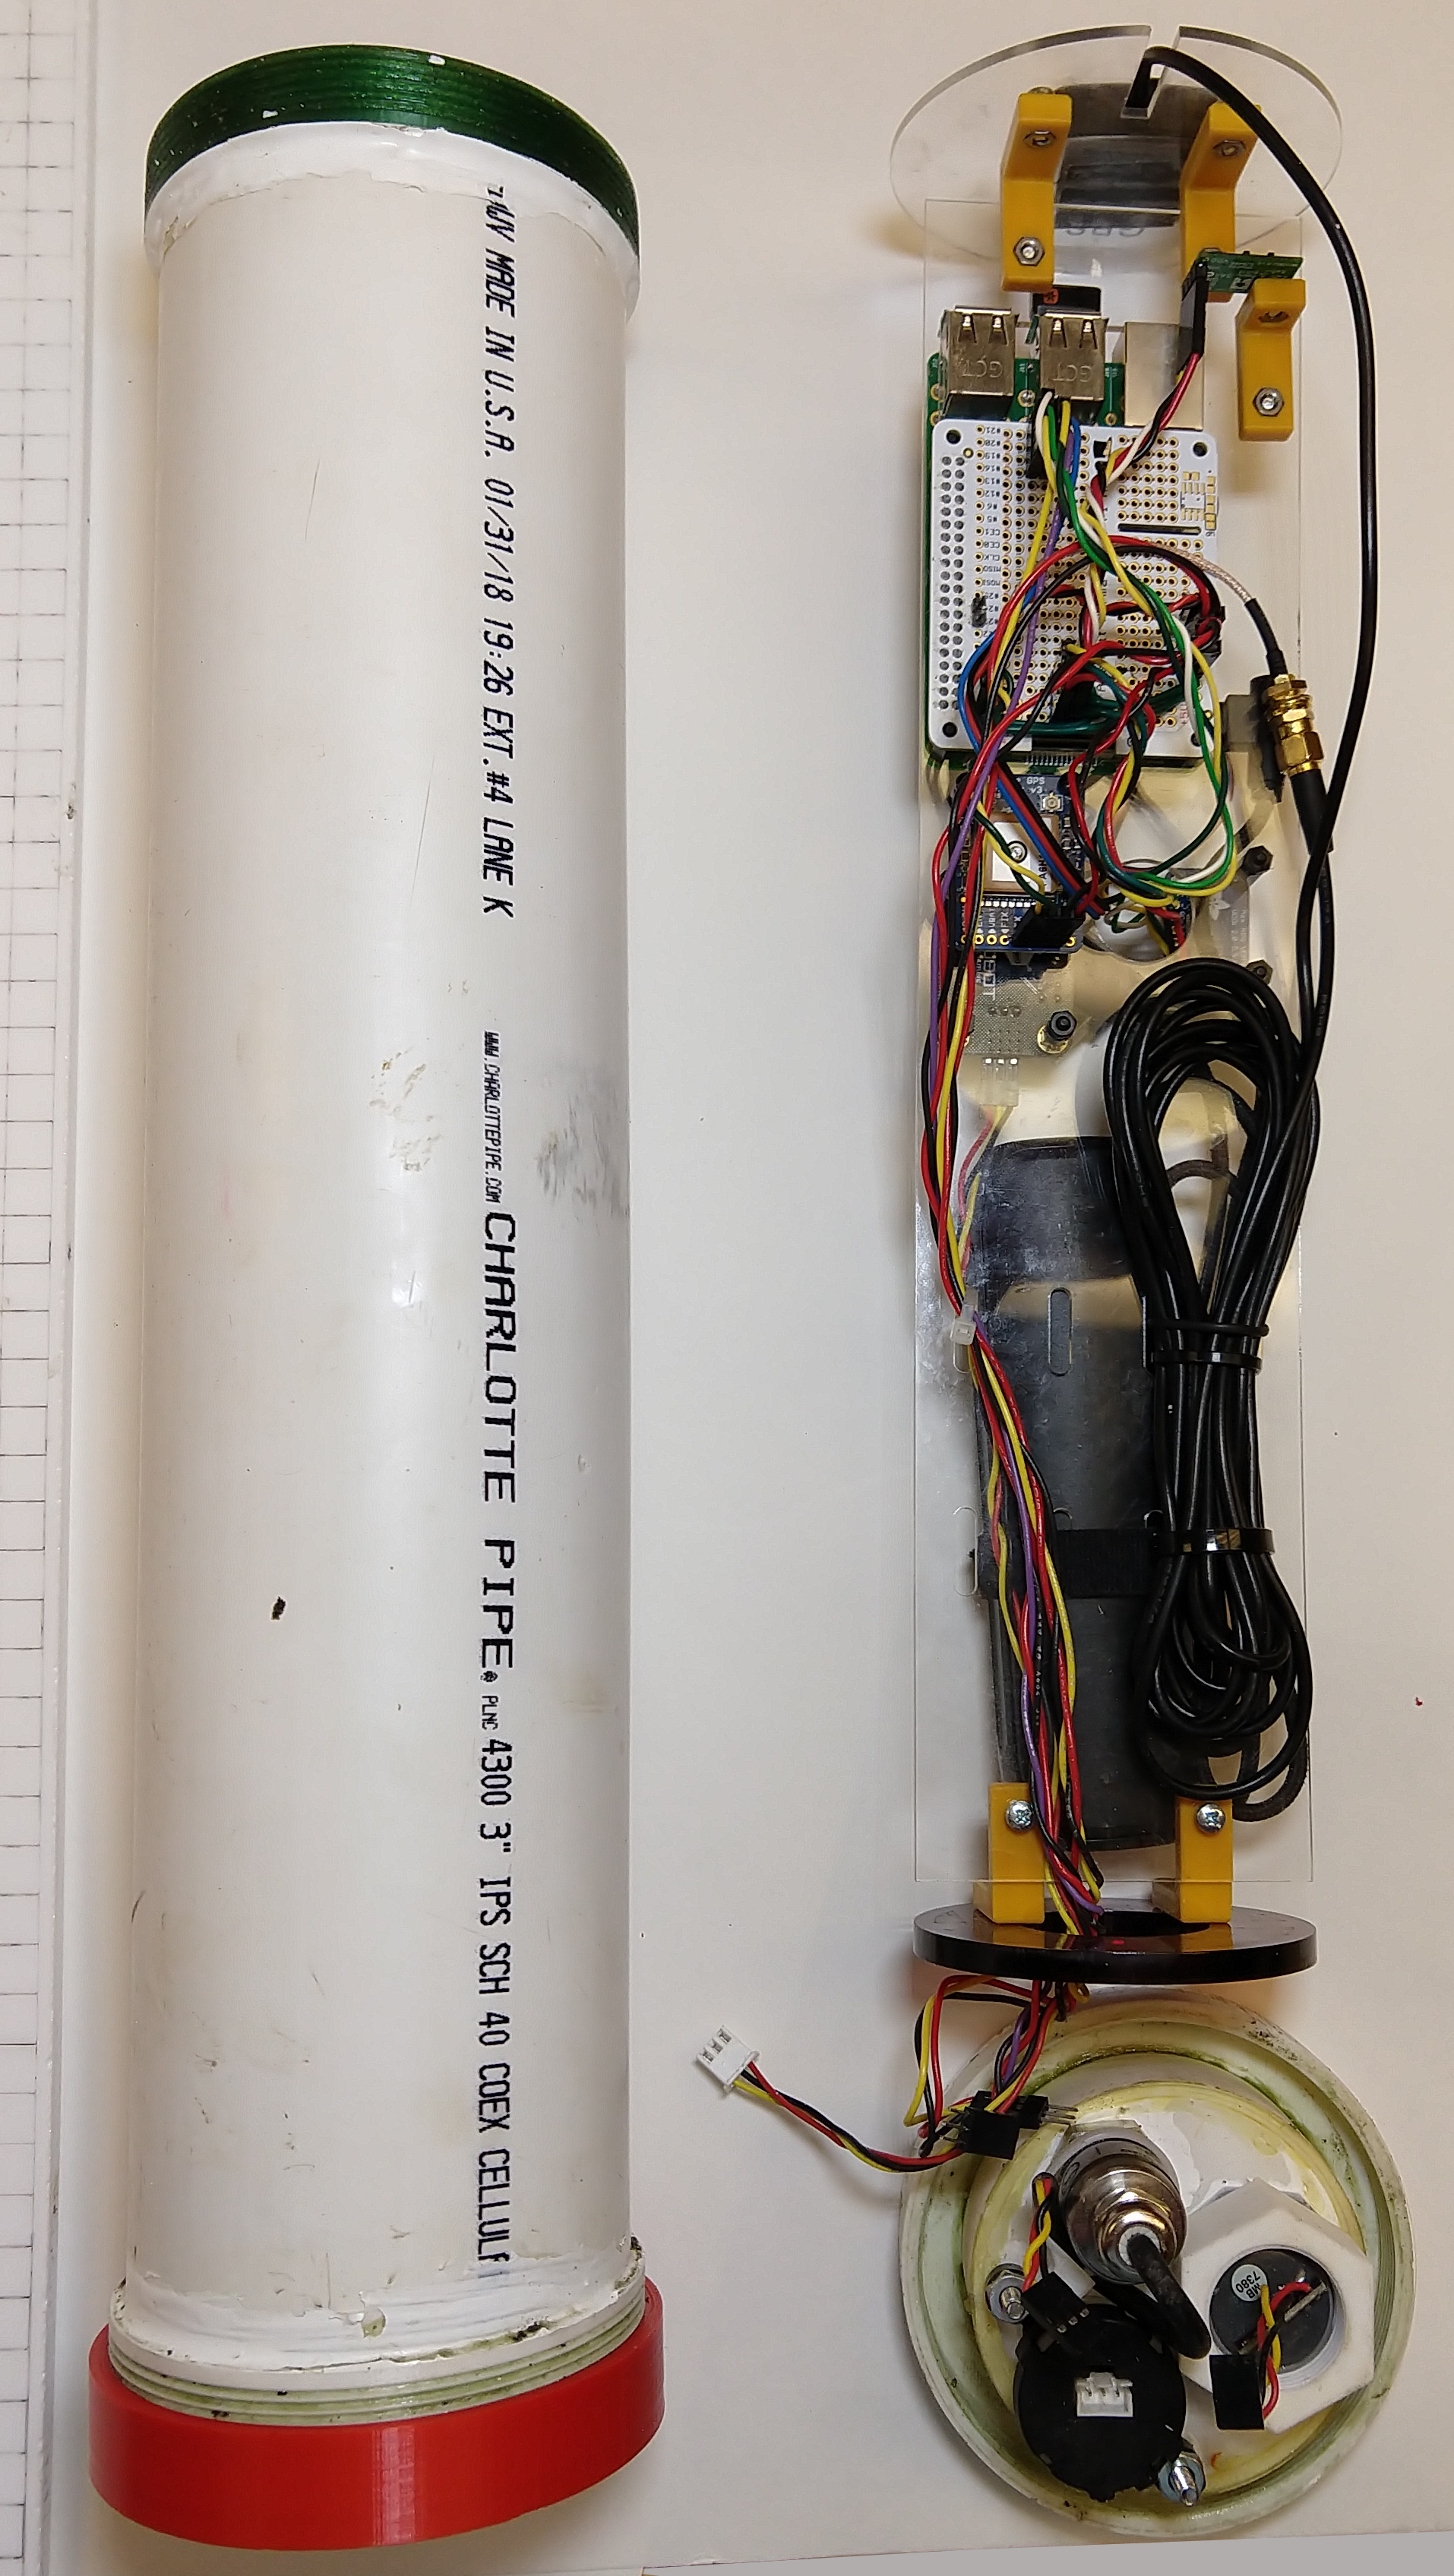
\includegraphics[height=12cm]{driftnode/driftnode.jpg}
	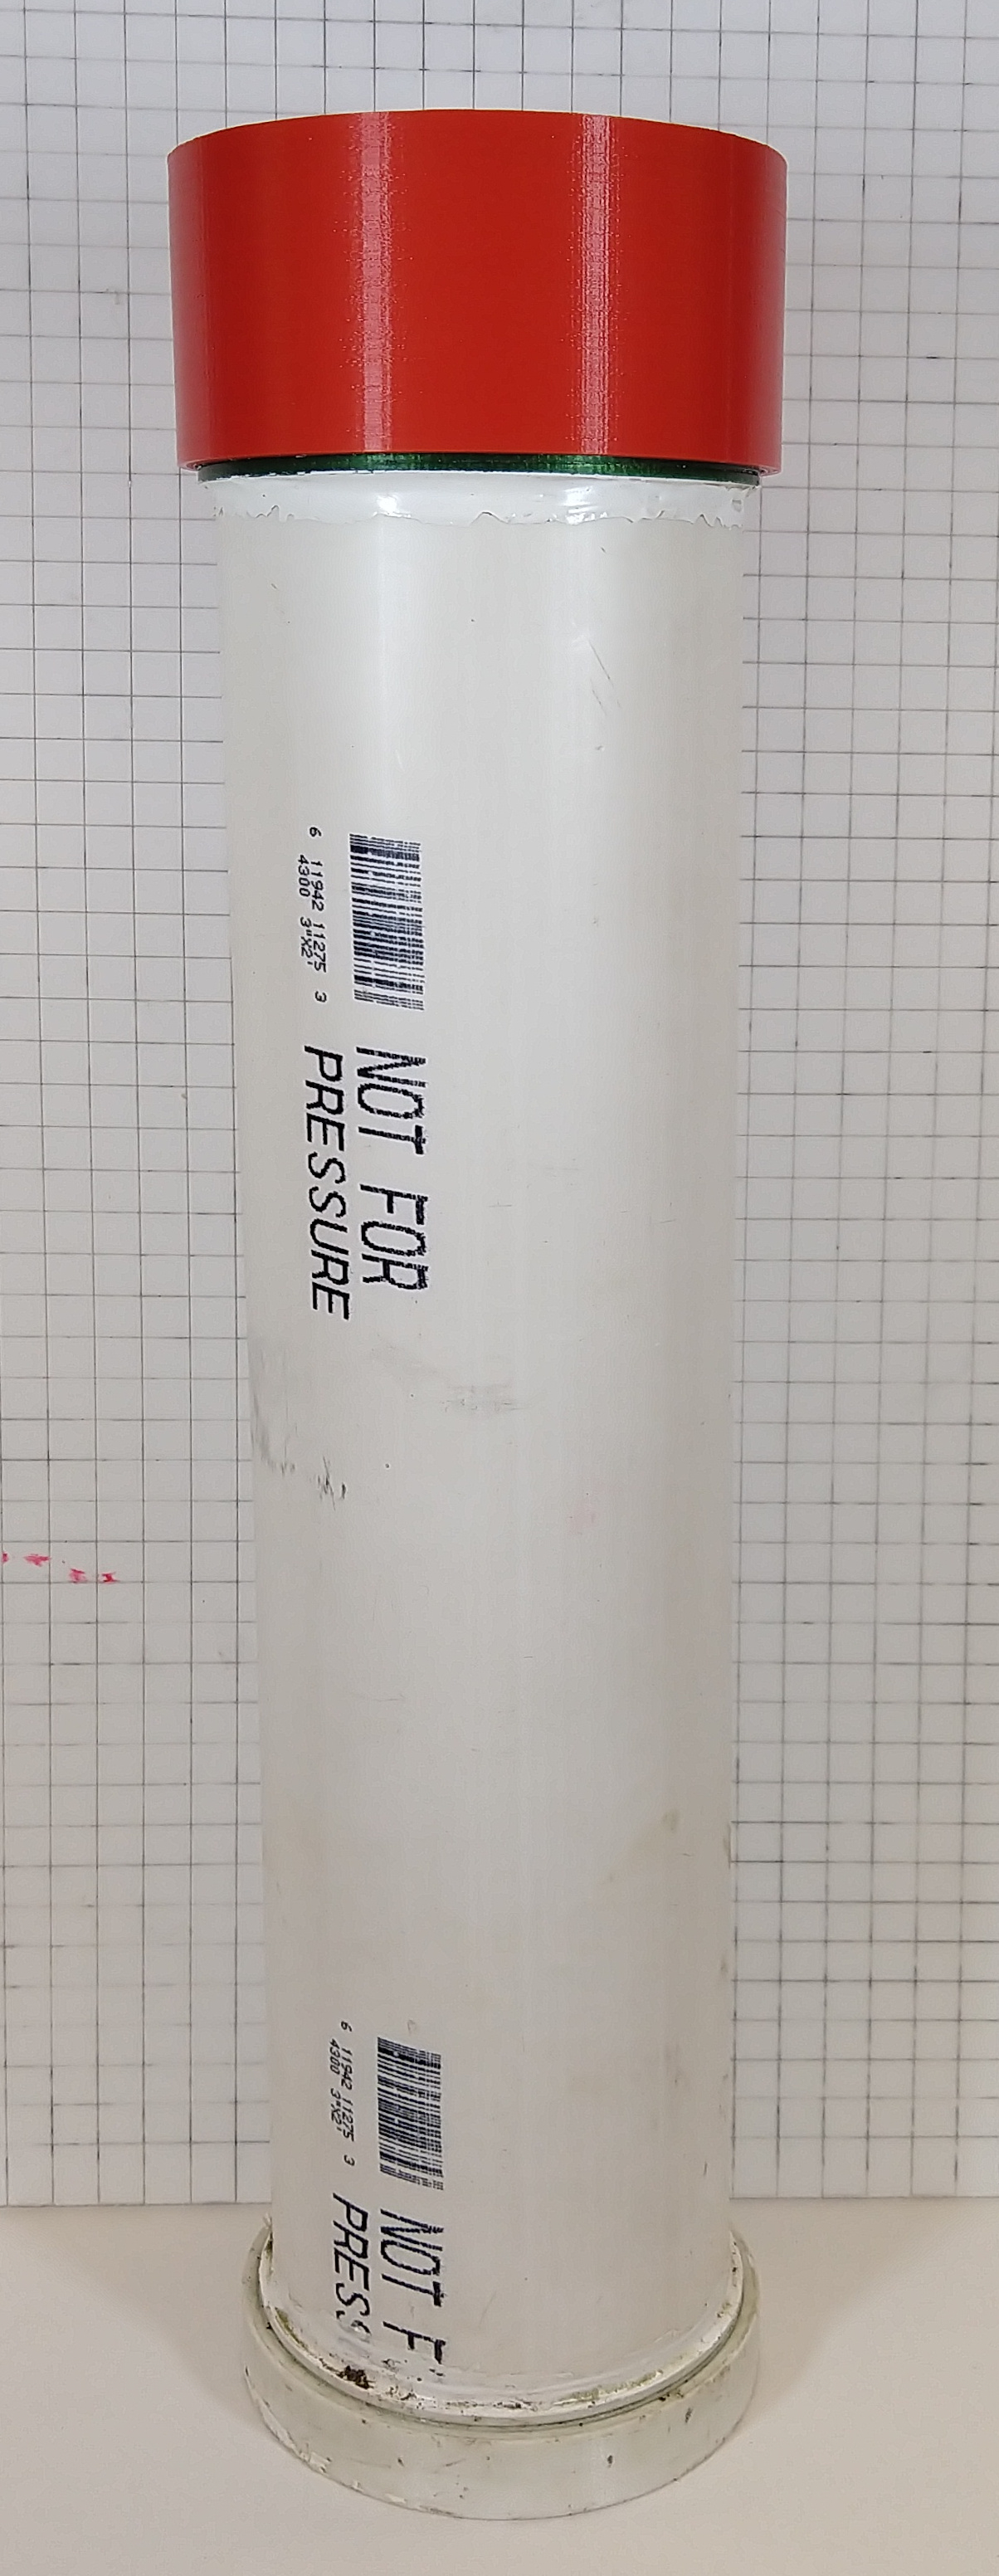
\includegraphics[height=12cm]{driftnode/driftnodeassembled.jpg}
	\caption[Driftnode]{
		(Left) driftnode before assembly, the electronics are attached to a center acrylic plate.
		(Right) an assembled driftnode.
	} \label{fig:driftnodeoverview}
	\end{center}
	\vspace{-1em}
\end{figure}

Humans knows less about the ocean than they do about space.
Because EM waves attenuate quickly in water, it is challenging to deploy wireless sensor network in water for permanent surveying post.
A boat and crew need to be dispatched to survey a water surface.
The crew can then manually deploy sensor at each location within the area for scientific research.
The team will need to be dispatched periodically to monitor an area for border security or fishing enforcement.
One crew cannot watch several areas simultaneously, so the man-hour required grow proportionally with area monitored.
This requires the need for several crews, or risk security incidence when an area is not monitored.

A wireless sensor network, composed of drifting sensors, deployed temporarily or permanently, can monitor an area for much longer with less labor needed.
A UAV can be used to periodically visit these sensors, collecting their sensor logs and charging them.
We present a drifting sensor platform, initially created by the University of South Carolina \cite{drifterUSC}, as seen in Fig.~\ref{fig:driftnodeoverview}.
The drifting sensor is composed of a suite of underwater sensor: An underwater depth sensor, a pressure sensor, a turbidity sensor, 9-axis IMU and GPS location sensor.
Our drifting sensor can broadcast its own wireless access point, which enables an AUV to collect data from the sensor at close range.

\chapter[UAV deploying Smartdarts]{UAV deployment of seismic microphones}

\section[Related Work]{Overview And Related Work}

This chapter presents a \emph{hetoerogenous seismic sensing system}, composed of stand alone geophone nodes deployed from unmanned aerial vehicles {UAV} and autonomous rovers with geophone attached.
We examine experimental data on geophone and soil coupling as a function of drop height and soil type.
We then provide a software tool for analyzing and planning a survey mission's logistic.
Our \emph{heterogenous sensor system} approach is designed to quickly and efficiently perform a survey with minimal manual labor for deployment and collection.

Sudarshan et al. \cite{sudarshan2015using} demonstrated a UAV equiped with four geophone sensors as landing gear.
The UAV in \cite{sudarshan2015using} can fly to a pre-programmed waypoint and land, attaching the geophones to the soil.

The geophones in  \cite{sudarshan2015using} had four problems:
(1) a UAV was required for each additional sensor,
(2) the force for planting the geophone was limited by the weight of the UAV,
(3) the platform required a level landing site,
(4) the magnets in the geophones distort compass readings, causing landing inaccuracy when autonomous.

The \emph{SeismicDart} presented in this system eliminates the need for a seperate UAV per sensor node.
Dropping the SeismicDarts from height also allows for greater penetration, firmer coupling and does not need a level landing site.
The new deployment unit also increase the distance between the SeismicDart's magnet and the UAV's magnetometer unit.

The SeismicSpider, our autonomous rover, can travel to survey locations inaccessible to UAV such as forests, thin atmosphere environments, caves or hard and rocky grounds which SeismicDarts cannot penetrate.
The SeismicSpider can also be deployed by a UAV, as close to the survey node as possible, then move to the desired location.

\subsection{Overview Of Seismic Sensing Theory}

\begin{figure}
	\centering
	\begin{overpic}[width=\columnwidth]{ral2016/Overview.pdf}\end{overpic}
	\caption{\label{fig:sensor_types}
	 Comparing state-of-the-art seismic survey sensors. a.) A traditional cabled system connects geophones in series to a seismic recorder and battery. b.) Autonomous nodal systems give each geophone a seismic recorder and battery.}
	%\vspace{-2em} 
\end{figure}



During seismic surveys, a source generates seismic waves that propagate under the earth's surface. 
These waves are sensed by geophone sensors and recorded for later analysis to detect the presence of resources. 
Fig.~\ref{fig:sensor_types} illustrates the components of current sensors. 

\subsubsection{Geophones}
Magnet-coil geophones contain a permanent magnet on a spring inside a coil. Voltage across the coil is proportional to velocity. 
 Beneath the coil housing is a metal spike. 
  Geophones are \emph{planted} by pushing this metal spike into the ground, which improves coupling with the ground to increase sensitivity. 
 The magnet-coil must be vertical. 
  Misalignment reduces the signal proportional to the cosine of the error.


\subsubsection{Cabled Systems}
Hydrocarbon exploration extensively uses traditional \emph{cabled systems} for seismic data acquisition.
Geophones are connected to each other in series using long cables. This cable is then connected to a seismic recorder and battery. 
The seismic recorder consists of a micro-controller which synchronizes the data acquired with a GPS signal and stores the data onboard. 
This method of data acquisition requires many manual laborers and a substantial expenditure for transporting the cables. 
Rugged terrain makes carrying and placing cables labor intensive, and the local manual labor pool may be unskilled or expensive.
   
\subsubsection{Autonomous Nodal Systems}
\emph{Autonomous nodal systems}~\cite{wood1998distributed} are now being used to conduct seismic surveys.
Unlike traditional cabled systems, autonomous nodal systems are not connected using cables.
The sensor, seismic recorder, and battery are all combined into a single package called a \emph{node} that can autonomously record data as shown in Fig.~\ref{fig:sensor_types}.
Even in these systems the data is generally stored in the onboard memory and can only be acquired after completing the survey.
This delay means errors cannot be detected and rectified while conducting the survey. 
Wireless autonomous nodes are a recent development.
These systems can transmit data wirelessly in real time~\cite{jiang2015geophysical}.
However, these systems still require manual laborers for planting the autonomous nodes at specific locations and deploying the large antennas necessary for wireless communication.
 
\subsection{Related Work}

Seismic surveying is a large industry.
The concept of using robots to place seismic sensors dates to the 1980s, when mobile robots placed seismic sensors on the moon~\cite{LSisMSE81}.
\cite{DSSMaA14} and \cite{coste2013seismic} proposed using a mobile robot for terrestrial geophone placement.
Plans are underway for a swarm of seismic sensors for Mars exploration~\cite{MAPL2006}.
Additionally,~\cite{muyzert2015marine} and~\cite{postel2014drone} proposed marine robots for hydrophone deployment underwater. 
Other work  focuses on data collection, using a UAV to wirelessly collect data from multiple sensors~\cite{wilcox2013seismic}.
Autonomous sensor deployment and mobile wireless sensor networks were studied in~\cite{howard2002mobile,corke2004autonomous,tuna2014autonomous}.
Heterogeneous mobile robotic teams were used for mapping and tracking in~\cite{howard2006experiments}.

\section[SeismicDarts]{SeismicDarts}

A SeismicDart combines a geophone (GS-100) with the fins and body of a lawn Jart\textsuperscript{TM}, using a 3D-printed chamber that encloses a WiFi-enabled microcontroller (particle.io Photon\textsuperscript{TM}) as shown in Fig.~\ref{fig:Smart_Dart_overview}. 
The center of the chamber is slotted to fit a wooden plate holding an accelerometer that transmits data wirelessly through the microcontroller. 
The centered accelerometer card allows placing the microcontroller and battery on opposite sides, balancing the dart.
Designs and instructions to build a SeismicDart are available at \cite{Victor2016Thingiverse}.



\begin{figure} \centering
{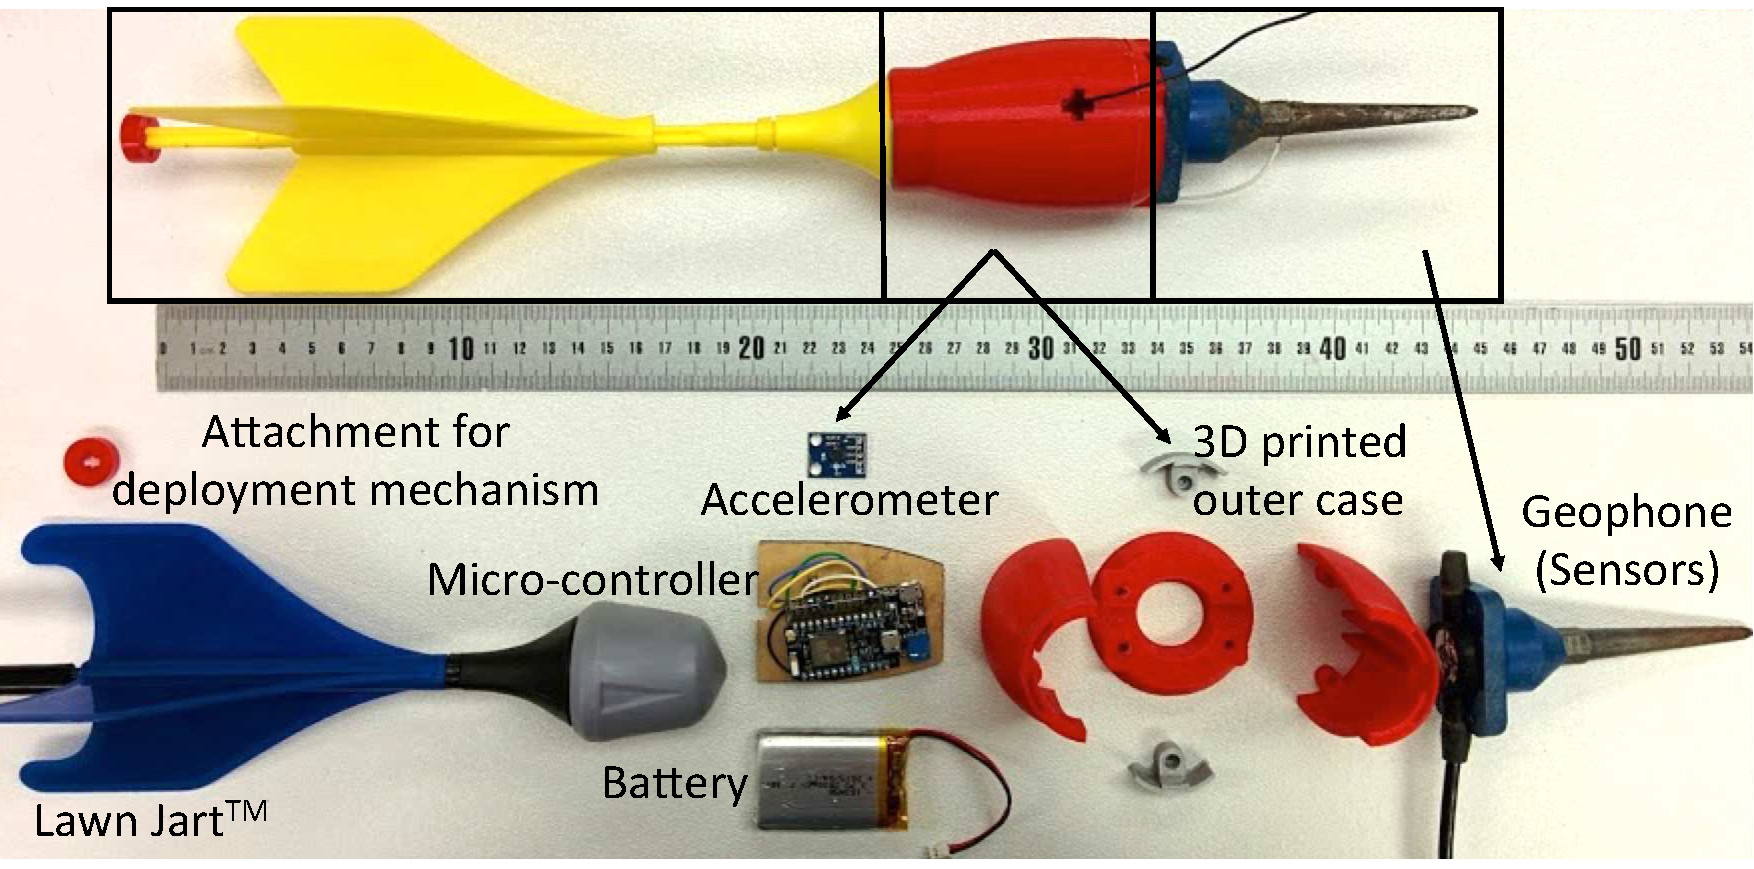
\includegraphics[width=\columnwidth]{ral2016/Smart_Dart_overview.pdf}}
\caption{Components of the SeismicDart sensor: a lawn  Jart\textsuperscript{TM} fin, particle.io Photon\textsuperscript{TM}  micro-controller, 3D printed protective casing, and a geophone.} 
\label{fig:Smart_Dart_overview}
\end{figure}

%%%%%%%%%%%%%%%%%%%%%%%%%%%%%%%%%%%%%%% 
\subsection{Experiments} 
The following sections compare SeismicDart performance.
\subsubsection{ Drop tests in different soils}  


Proper planting of a geophone requires good contact with the soil and the geophone to be in a vertical position. 
Geophone protocol classifies a geophone as well planted if the angle of deviation is less than 10$^\circ$ and the spike has at least 40 mm of penetration.

To determine how SeismicDarts perform in different soils, this experiment measured penetration depth and angle of deviation in seven different soil types as a function of drop height. 
 The soil types were categorized by compression strength, in kg/cm$^2$, measured using a soil pocket penetrometer (CertifiedMTP). Measurements for compression strength vary with a small deviation in measurement location, so we repeated this measurement 10 times at 10 different locations in each soil type and computed the average.
 
 Experiments were conducted using the UAV to autonomously drop a payload of four SeismicDarts at the desired drop height. 
 Tests were conducted at drop heights of 10, 15, 20, and 25 m. 
 We measured the angle of deviation and penetration depth for each drop.
 The angular deviation was measured using two protractors.
 We measured penetration depth by marking where the spike met the soil, pulling the dart from the soil, and measuring the distance from the spike tip to the marking with calipers. 
  We repeated this measurement 12 times for each soil type at each drop height.  The soil compression strengths in these experiments ranged from 0.056 kg/cm$^2$ for river sand, to 4 kg/cm$^2$ for a hard-packed soccer field.

Because the four soil types with the lowest soil compression strength could be well-planted with low drop heights, we performed these tests manually. 
We filled 19 liter (5 gal.) buckets with four soil types and dropped the SeismicDart from six heights.
%Penetration depth and angular deviation were measured. %To measure penetration depth, the buried darts were marked where the spike met the soil, the dart was then pulled from the soil, and the distance from the spike tip to the marking was measured with calipers. The angular deviation was recorded using the accelerometer inside the dart.

 
  % These experiments shows that increasing drop height increases penetration on all soils tested.
  % Also, darts dropped in quiescent air remain vertical if they penetrate the soil.
Experiment results plotting penetration depth as a function of drop height are displayed in Fig.~\ref{fig:DepthPlotIndoors}, and angle of deviation as a function of drop height in Fig.~\ref{fig:AnglePlotIndoors}.   Both graphs are annotated with values for soil compression strength. 

\begin{figure} \centering
{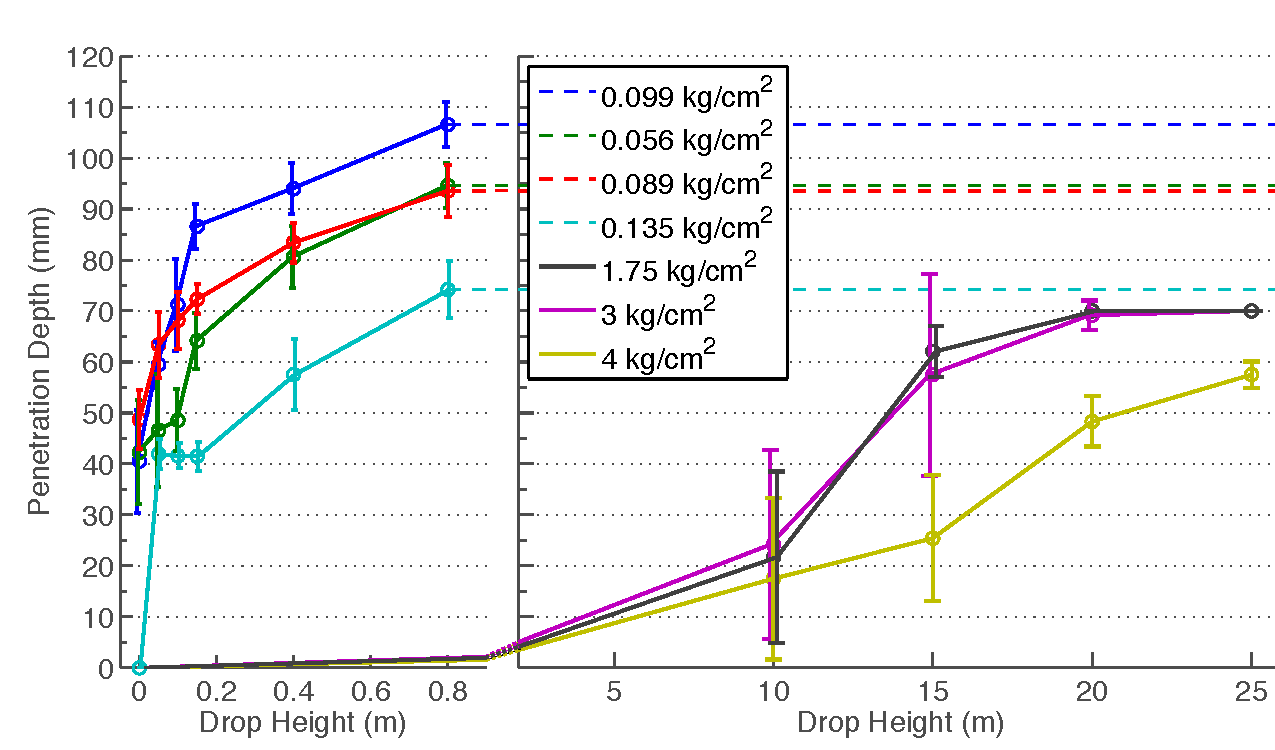
\includegraphics[width=\columnwidth]{ral2016/AutoPenetrationDepth2.pdf}}
\caption{Drop height vs. penetration depth in seven soil types. Drops were performed autonomously and each data point represents 12 trials. Increasing the drop height increased the penetration depth for all seven soil types.} 
\label{fig:DepthPlotIndoors}
\end{figure}

\begin{figure} \centering
{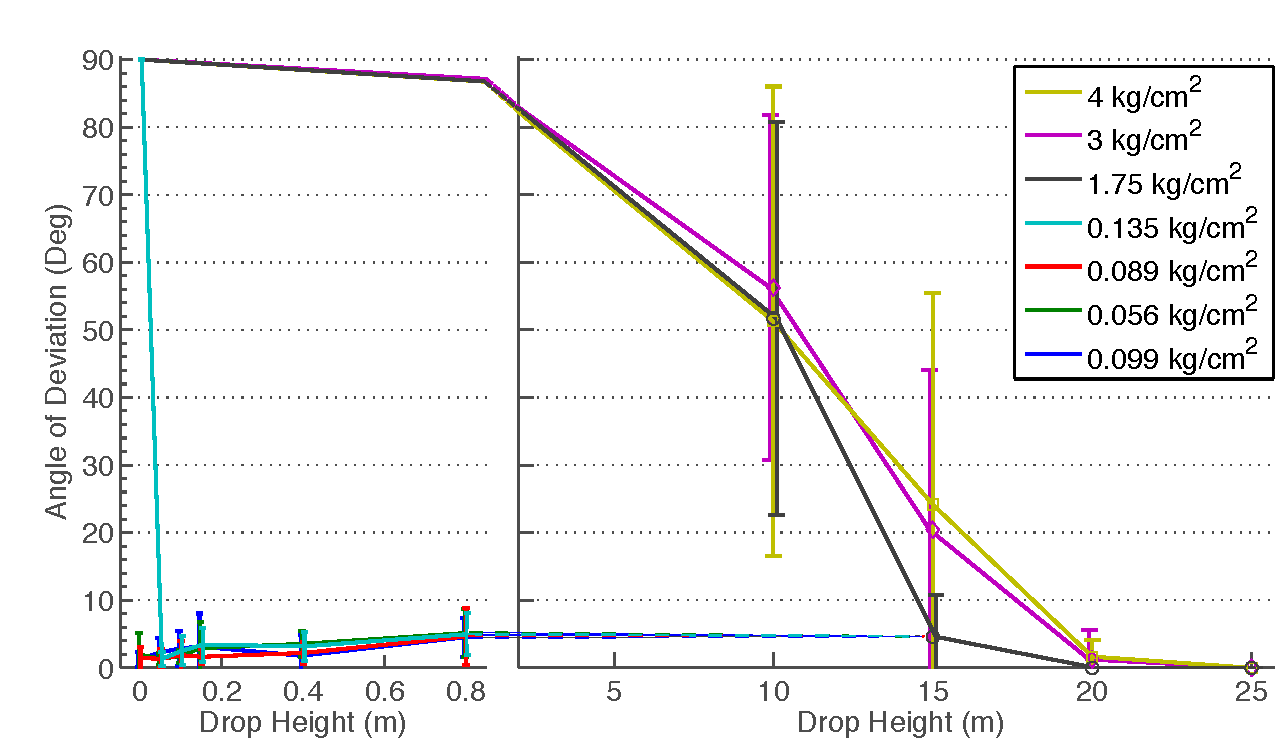
\includegraphics[width=\columnwidth]{ral2016/AutoPenetrationAngle2.pdf}}
\caption{Drop height vs. angle of deviation in seven soil types. Drops were performed autonomously and each data point represents 12 trials. Increasing the drop height reduced the angle of deviation for all seven soil types.} 
\label{fig:AnglePlotIndoors}
\vspace{-1em}
\end{figure}

If a SeismicDart is dropped from a sufficient height into penetrable soil, the spike will be buried into the soil and the geophone will have a small angular deviation from vertical. Soils with higher compression strength require higher drop heights. Error bars show that variance decreases with drop height for angle of deviation and penetration depth.  
 All drops from heights 20 m or more achieved the goals of an angle of deviation less than 10$^\circ$ and at least 40 mm of penetration.   

The autonomous tests were conducted with 16 km/hr winds, demonstrating that drop heights 20 m or higher were sufficient to counter disturbances from the wind. %https://www.windfinder.com/forecast/galveston_airport

\subsubsection{Shot gather comparison} 
Geophysical explorationists often use thousands of geophones to conduct a seismic survey. 
 As a proof-of-concept, this experiment ran a small-scale seismic survey to compare the performance of a traditional cabled four geophone system with readings from four autonomously deployed SeismicDarts.
Flying autonomously at a drop height of 25 m, the UAV flew to GPS waypoints spaced 4 m apart and deployed one dart at each location. 
A seismic survey technician manually planted four traditional cabled geophones, each 10 cm from a deployed SeismicDart. 
A seismic wave was generated using a sledgehammer hitting a steel plate.

Results of the field test comparison between the traditional cabled geophone system and the SeismicDarts are shown in Fig.~\ref{fig:shotgather_auto_drop}.   
Data were obtained using a \emph{StrataVisor}, a device that can obtain, store, and plot the sensed data. 
The \emph{StrataVisor} is extensively used with traditional geophone setups because the geophones can only sense vibrational waves and are dependent on other devices for storage and data processing. 
To allow a fair comparison with geophones, the SeismicDart's  ability to store sensed data was not used in this experiment. 
 The \emph{StrataVisor} records the geophone voltage at 2000 Hz, using a 24 bit ADC.

The readings from both systems are qualitatively similar, with no discernible phase or amplitude differences. Let $X$ be measurements from the traditional geophone and $Y$ the corresponding voltages from a SmartDart.
The percent peak-to-peak error and normalized root-mean-square error (NRMSE) are defined as
\begin{align}
e_{pp} &= 100 \left( \frac{ \max(X) - \min(X) }{ \max(Y) - \min(Y) } -1\right) \\
  \text{NRMSE} &=\frac{100}{\max(X) - \min(X)} \sqrt{ \frac{ \sum_{i=1}^n \left( X_i - Y_i \right)}{n} }.
\end{align}
The peak-to-peak errors were [-6.33, -1.15, -1.81,  9.84] \% for sensors at [4,8,12,16] m from the source.
 The NRMSE were [1.05,1.27,3.98,4.39] \% for sensors at [4,8,12,16] m from the source.
%$e_{\text{4 m}}  =  -6.3 \%, e_{\text{8 m}}  =  11.93 \%, e_{\text{12 m}}  = -1.81\%, e_{\text{16 m}}  = 0.981 \%$. 
%The RMSD error were $RMSD_{\text{4 m}}  =  -6.3 \%, RMSD_{\text{8 m}}  =  11.93 \%, RMSD_{\text{12 m}}  = \%, RMSD_{\text{16 m}}  = 0.981 \%$. 
Readings were also compared using a Pearson product-moment correlation coefficient, which gives a correlation measurement between $-1$ and $+1$ where $+1$ is total positive linear correlation:
\begin{align}
\rho_{X,Y} = \frac{E\left[  (X-\mu_X) (Y-\mu_Y)  \right]}{  \sigma_X, \sigma_Y}.
\end{align}

The correlation coefficients were $\rho_{\text{4 m}}  =  0.9813, \rho_{\text{8 m}}  =  0.9836, \rho_{\text{12 m}}  =  0.8600, \rho_{\text{16 m}}  = 0.8114$. These correlations decrease with distance. The SeismicDart is subject to low-amplitude noise, which is easiest to see in the fourth sensor because it was 16 m from the seismic source and thus had the lowest signal amplitude.  This noise is potentially due to wind striking the SeismicDart's fin. The effect of noise can be mitigated by using larger seismic sources such as a vibration truck or explosives.



\begin{figure} \centering
  {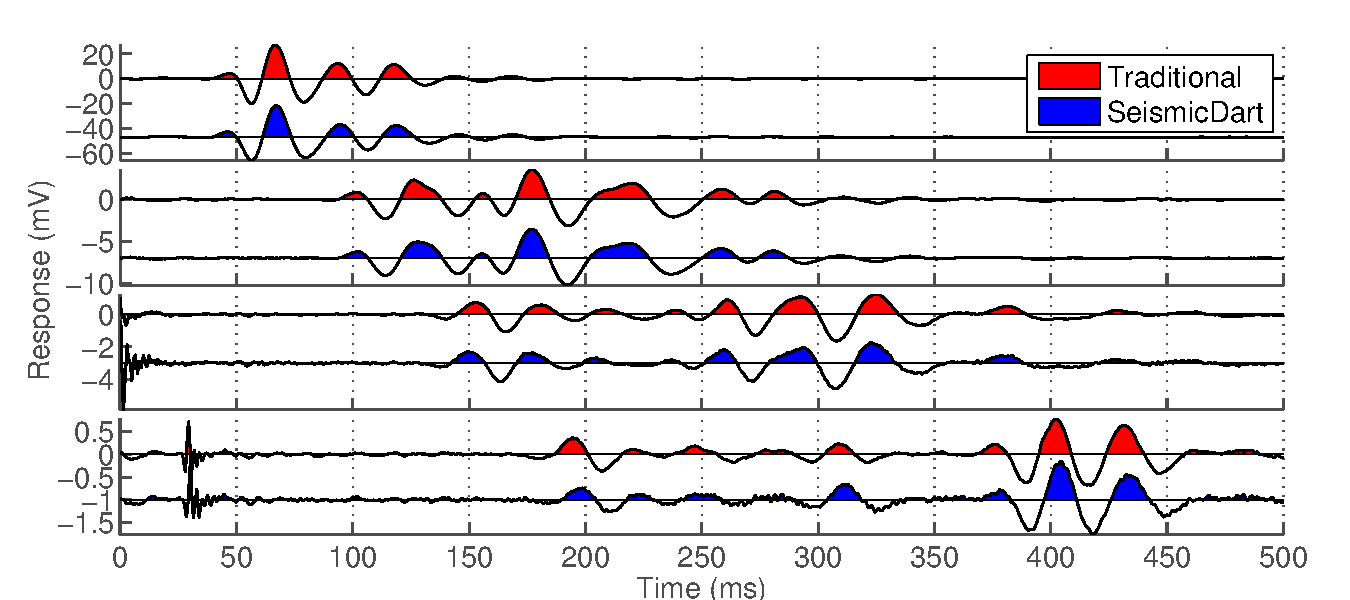
\includegraphics[width=\columnwidth]{ral2016/SeismicSurveyComparison.pdf}}
 \caption{Raw voltage data from shot gather comparison of four traditional geophones and four autonomously dropped SeismicDart sensors.  
 \label{fig:shotgather_auto_drop}}
\end{figure}

\subsection{SeismicDart Deployment and Retrieval}
First, the SeismicDarts are loaded onto to a UAV. 
Currently, a maximum of four sensors can be dropped in a single flight. 
The flight plan communicated to the UAV provides a GPS waypoint for each SmartDart. 
The UAV flies to and drops a SmartDart at each waypoint, then returns home. 

Deployment is only one part of a survey. Large surveys require moving and reusing sensors.  
Because SmartDarts are more expensive than standard geophones, rapid reuse is essential.
The UAV has an underslung hook for picking up a SeismicDart.
Retrieval is facilitated by attaching a wire loop to the SeismicDart tail.
 This loop provides a target 300 mm in diameter for the hook, yet still allows autonomous deployment, as shown in Fig.~\ref{fig:SeismicDart_DR}.
Currently, retrieval is performed by manually piloting the UAV, but the loop size is within the accuracy of a UAV equipped with RTK GPS.
%Automating retrieval is out of the scope of this paper.



\begin{figure} \centering
  {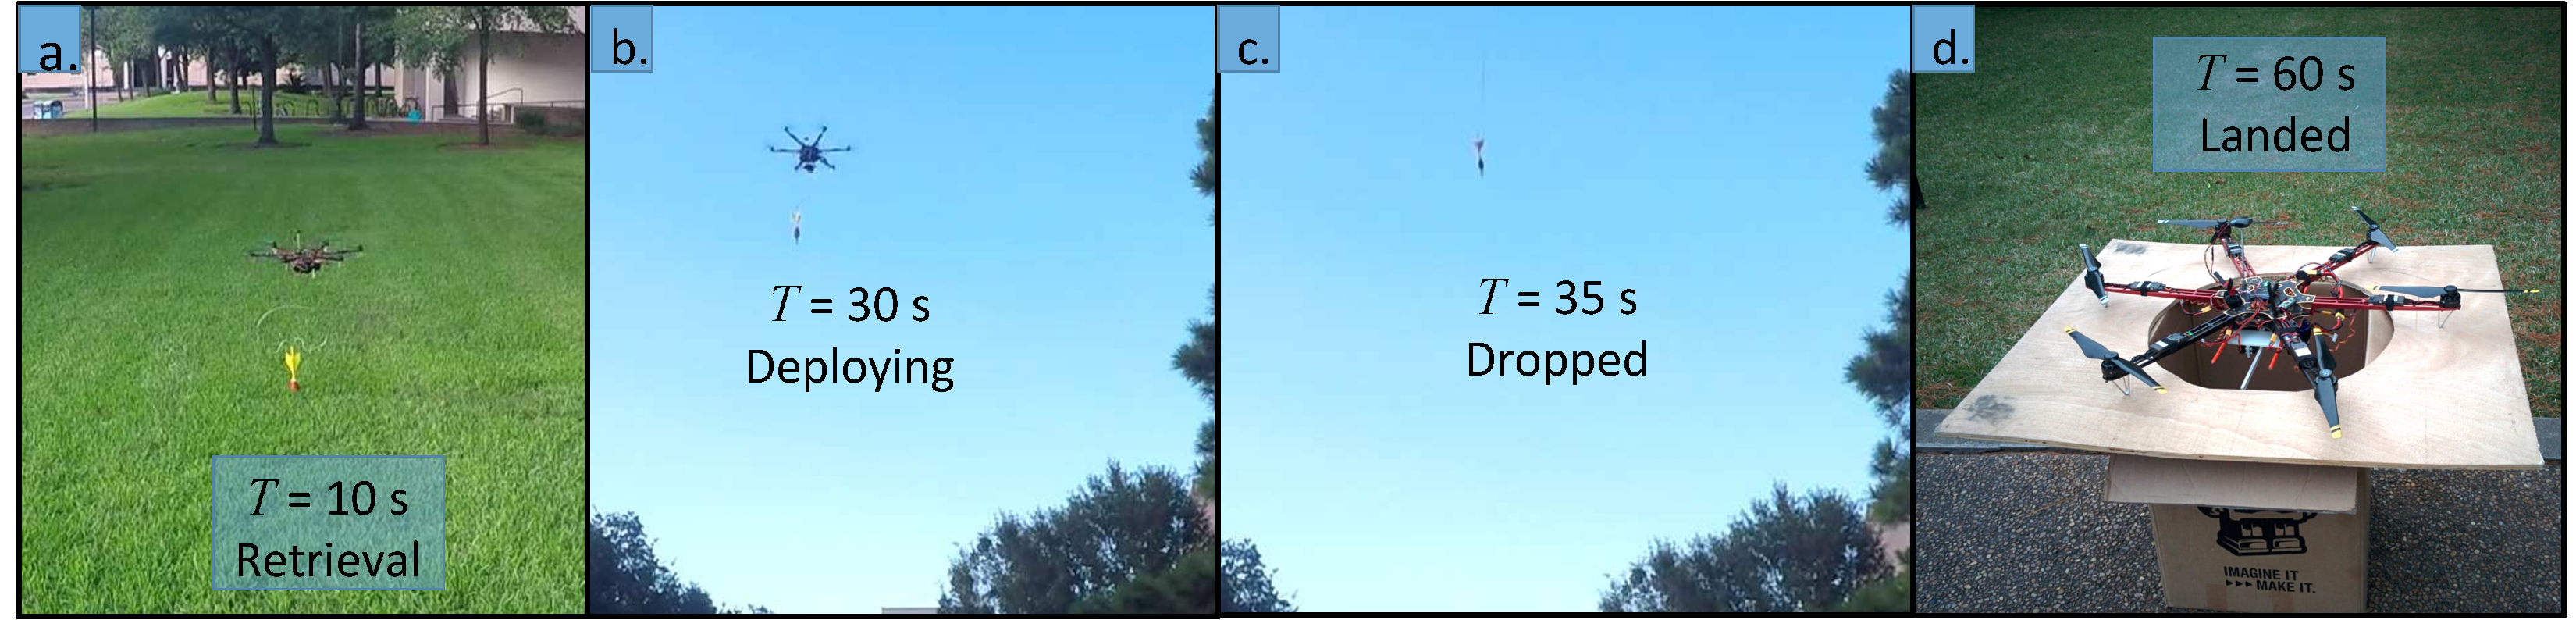
\includegraphics[width=\columnwidth]{ral2016/SeismicDart_DR.pdf}}
 \caption{SmartDart retrieval and redeployment.  See video attachment. 
 \label{fig:SeismicDart_DR}}
\end{figure}
 

\section{SeismicSpider}\label{sec:SeismicSpider}


\begin{figure} \centering
  {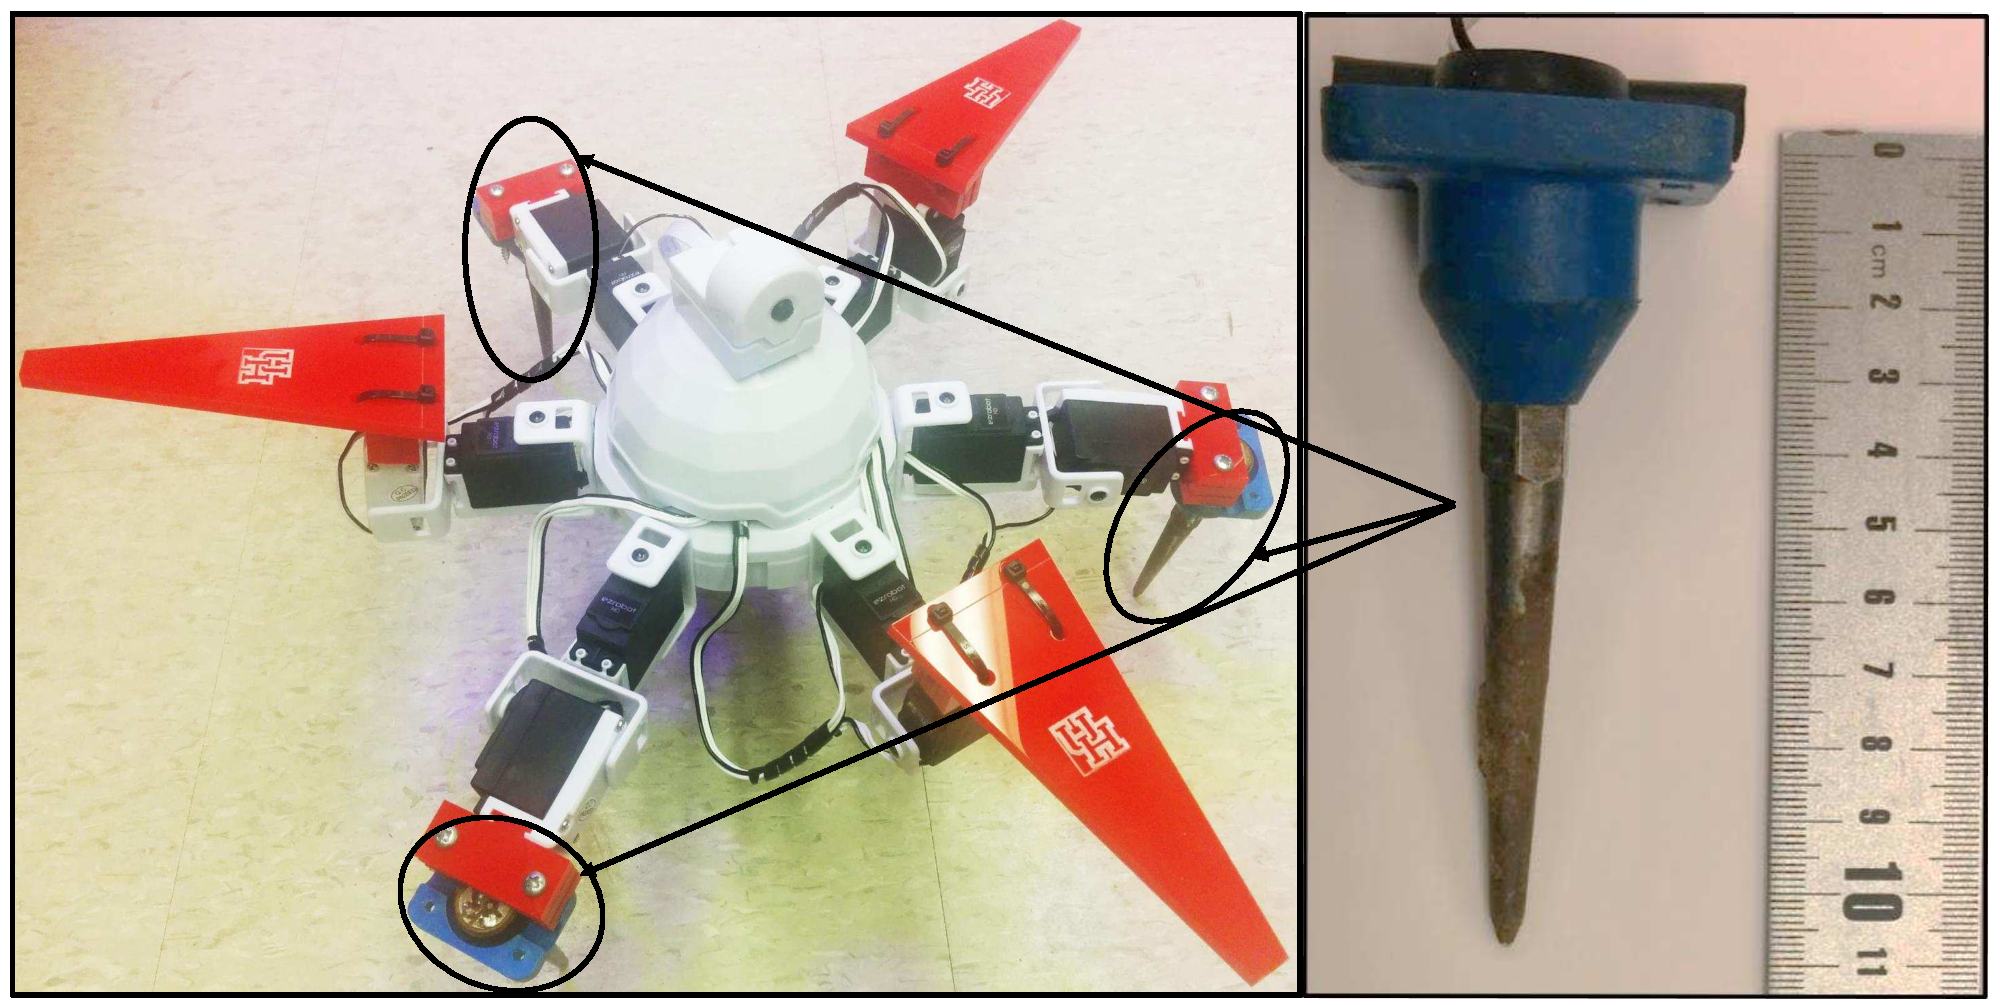
\includegraphics[width=\columnwidth]{Hex_overview.pdf}}
 \caption{The SeismicSpider is a six-legged mobile robot where geophones replace three legs. It is drone deployable, can sense and record seismic data, and can move to desired locations, including terrain the SeismicDart cannot access.} 
 \label{fig:Hex_overview}
\end{figure}


The SeismicSpider, shown in Fig.~\ref{fig:Hex_overview}, is built from the Six Hexapod kit designed by EZ-Robots. Each of the six legs is powered by two 15 kg$\cdot$cm lever servos. Three legs were replaced by three GS-20DM 14 Hz geophones from Geospace Technologies. The remaining three legs were designed to match the geophone dimensions.

 Our initial plan to use three geophones required the spider to raise the three inactive legs while acquiring data. This lack of support caused excessive strain on the three servo motors responsible for holding the spider upright, introducing unwanted vibration into the system.  Positioning the geophone legs at 20$^\circ$ to normal enhances stability and relieves the excessive stress on the servos. 
 The three geophones were in series, so with each geophone leg angled inward, superposition replicates the signal from one vertical geophone.
 
 Traditional geophones are mounted in an insulated, shock-resistive enclosure on a spike. The spikes, varying in length, are inserted into the ground to ensure a firm coupling with the environment. The design of our SeismicSpider prevents full depth insertion of the 88 mm spikes. 

	To overcome the coupling issue we are using three geophones per station compared to the typical one. Our immediate goals were to compare amplitude response to that of a standard single station.	
 

\subsection{Shot gather comparison}
%\subsubsection{Accuracy plot}
%Hexapod move to desired GPS location  (plot accuracy)\\
%\subsubsection{ Shot gather comparison}

A line of twenty-four geophones (GS-20DM 14 Hz) were laid out at one-meter intervals with our inline source seven meters from the nearest geophone. Beginning from the farthest offset of 31 m we manually aligned the Spider with the corresponding geophone, fired the source, then moved one meter ahead. 

%\paragraph{Results}
Data from the shot gather comparison is shown in Fig.~\ref{fig:shotgatherHexpod}.
The response for three geophones in series was 5 dB greater than a single geophone. The geophone wires proved insufficient to insulate against 60 Hz noise. Hence the raw data from the traditional setup as well as the SeismicSpider was processed with a (3-50) band-pass filter. Finally, the SeismicSpider data was attenuated by $-5$dB to level the comparison.    

\begin{figure} \centering
  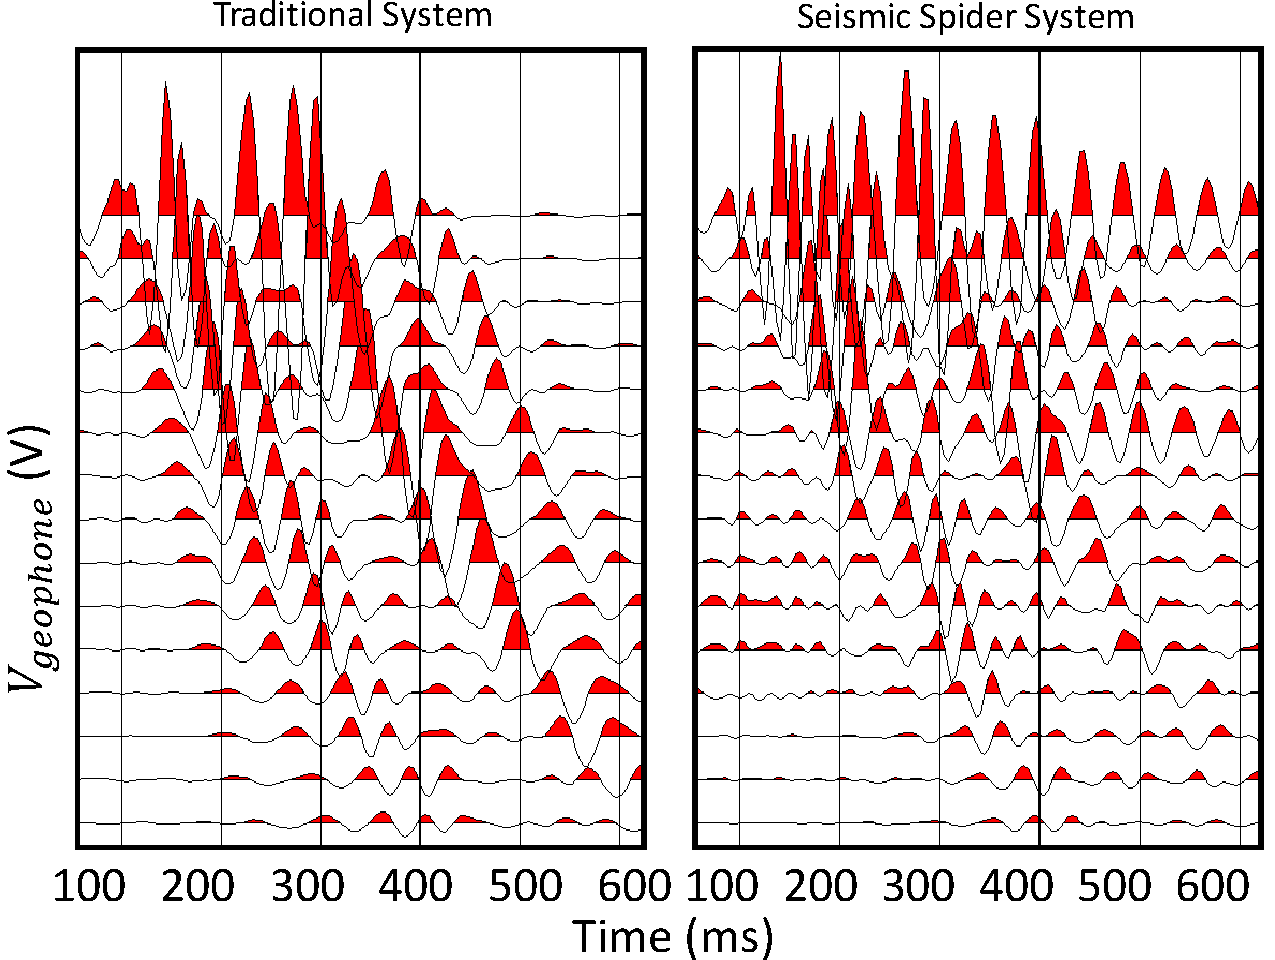
\includegraphics[width=\columnwidth]{shotgather_hex.pdf}
 \caption{Shot gather comparison of traditional geophones vs. SeismicSpider. 
 \label{fig:shotgatherHexpod}}
\end{figure}

%\paragraph{Future work}	we must filter 60 Hz noise, compare adding geophones to all six legs, and design a larger seismic survey to ensure adequate data for phase analysis. Design improvements could be done to make the SeismicSpider an active sensor.   


\subsection{Deploying and Retrieving the SeismicSpider}

\begin{figure} \centering
  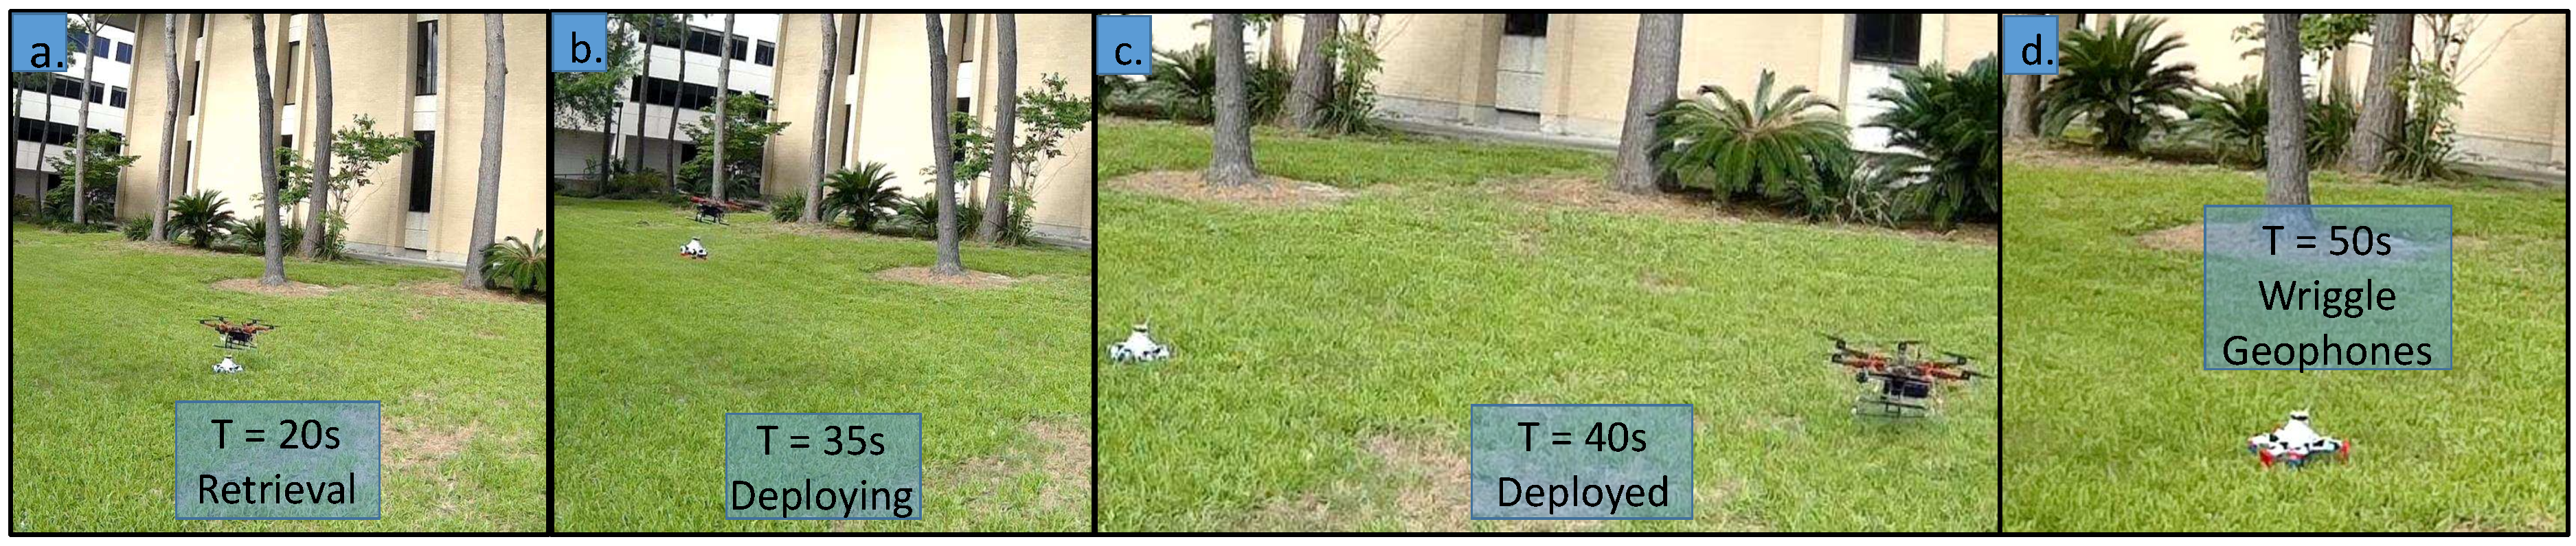
\includegraphics[width=\columnwidth]{SeismicSpider_DR.pdf}
 \caption{SeismicSpider retrieval and redeployment. See video attachment. 
 \label{fig:SeismicSpiderDR}}
\end{figure}

The UAV's purpose is to deploy sensors at desired GPS waypoint locations. The SeismicSpider is a mobile robot, but it is substantially slower than the UAV.  The UAV carrying the SeismicSpider flew autonomously to a programmed waypoint. The deployment mechanism included a hook controlled by a servo attached to the UAV. The UAV lowered to a waypoint 0.5 m from the ground, then the servo was triggered to unhook the SeismicSpider.  The SeismicSpider was then wirelessly powered on. 
The SeismicSpider also has an onboard GPS, enabling it to navigate to desired waypoints. 
After walking to the sensing location, the SeismicSpider was programmed to shake its three non-sensing legs to plant its geophone legs into the ground.  
  Currently, autonomous deployment of sensors is implemented, but the retrieval is piloted. 
Combining the mobility of the SeismicSpider with the speed of the UAV enables reaching locations inaccessible by air or impossible to penetrate by SmartDarts.
Fig.~\ref{fig:SeismicSpiderDR} shows the SeismicSpider being retrieved and then redeployed by a UAV.






\section{UAV and deployment unit}\label{sec:DeploymentUnit(UAV)}

The UAV is a custom-built, 1.77 m wingspan hexacopter, controlled by a Pixhawk flight controller running ArduPilot Mega flight software. The UAV has a 3DR GPS module using the UBlox NEO-7 chipset.


 The deployment mechanism allows the UAV to carry four SeismicDarts in a circular array, and release them when it reaches the desired GPS location, one at a time.
 The rear of the dart has a circular tip that locks into the deployment mechanism, and rests on a rectangular slot-path. 
 A servomotor rotates the dart tips through the rectangular slot-path, allowing darts to release from a circular opening,  as shown in Fig.~\ref{fig:deployment_system}.



\begin{figure} \centering
  {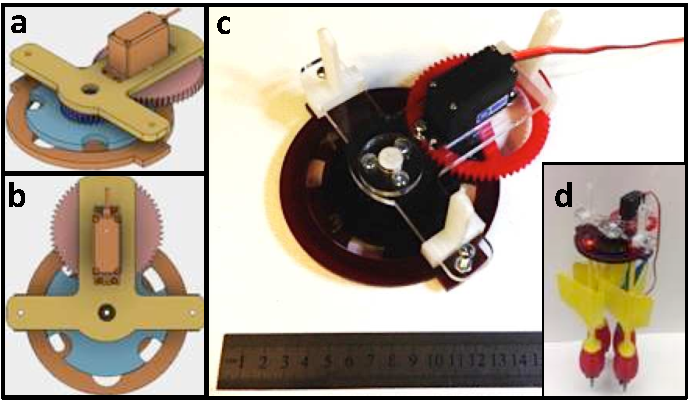
\includegraphics[width=\columnwidth]{deployment_system.pdf}}
 \caption{Deployment system for dropping SeismicDarts from the UAV. Pictured design holds four darts, but can be scaled according to the UAV's carrying capacity.} 
 \label{fig:deployment_system}
\end{figure}




\subsection{Autonomous drop demonstration and accuracy}

The current UAV can place a SeismicDart within $\pm1$ m of the desired location.  
This range is within tolerances for seismic surveys because often features (rocks, water, etc.) exist that require this amount of error from theoretically assigned locations and some survey designs include a random placement component to improve noise cancellation.
%(3) this error minimally perturbs the data since seismic waves travel at 600 m/s near the surface, so a one-meter inaccuracy equates to $\approx$1.6 ms delay.
%(4) the response of a receiver to seismic vibrations is an average over a number of meters.  ?? what does this mean??

To accurately perform a seismic survey, the sensors do not need to placed accurately, but their position must be known within $\approx$ 0.01 m. 
 Knowledge of the exact location compensates for placement inaccuracy.
 Localization can be achieved by placing an RTK GPS in each dart.  A lower-cost solution would use an RTK GPS on the SeismicDrone and perform image registration with the downward facing camera.  As shown in the multimedia attachment, even at a 25 m drop height a planted dart occupies dozens of pixels, enabling cm-level localization accuracy.


%allows corrections for jitter in signal arrival times due to  placement inaccuracy.


%Exp 4: Automatic drop from drone, accuracy in placement
\begin{figure} \centering
  {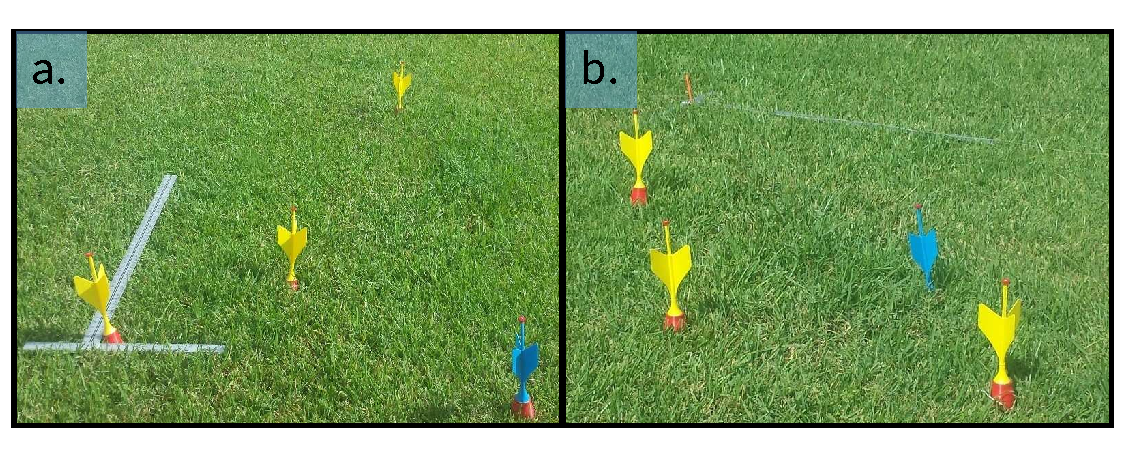
\includegraphics[width=\columnwidth]{accuracy_test_overview.pdf}}
 \caption{a.) First set of darts with reference axes. b.) Third dart set. } 
 \label{fig:Accu_test_darts}
\end{figure}

For the accuracy test, six sets of darts, four darts in each set, were dropped on the same GPS waypoint. Between each drop, the UAV traveled to a nearby GPS waypoint to cancel out the flight controller's stable hover.
The UAV then returned to the launch platform to be reloaded, we recorded the dart landing positions, collected the darts, and reloaded the darts on the UAV for the next deployment set.
The measurement method of the darts' positions are shown in Fig.~\ref{fig:Accu_test_darts}.
Results are shown in Fig.~\ref{fig:SD_accu.pdf}.
  
%To measure position, one dart was picked from the first set as the reference point (the lower left in Fig.~\ref{fig:Accu_test_darts}b), hence the first data point was (0,0). A 1-m T-square was placed with the origin at the dart's drop point to establish reference axes.


 %A rod was placed in the position of the first dart to keep reference as shown in Fig.~\ref{fig:Accu_test_darts}c. 
% The T-square was kept in place and mason twine was suspended to lengthen the reference axes. 
% Future deployments were measured  using the reference point and axes. 



\begin{figure} \centering
  {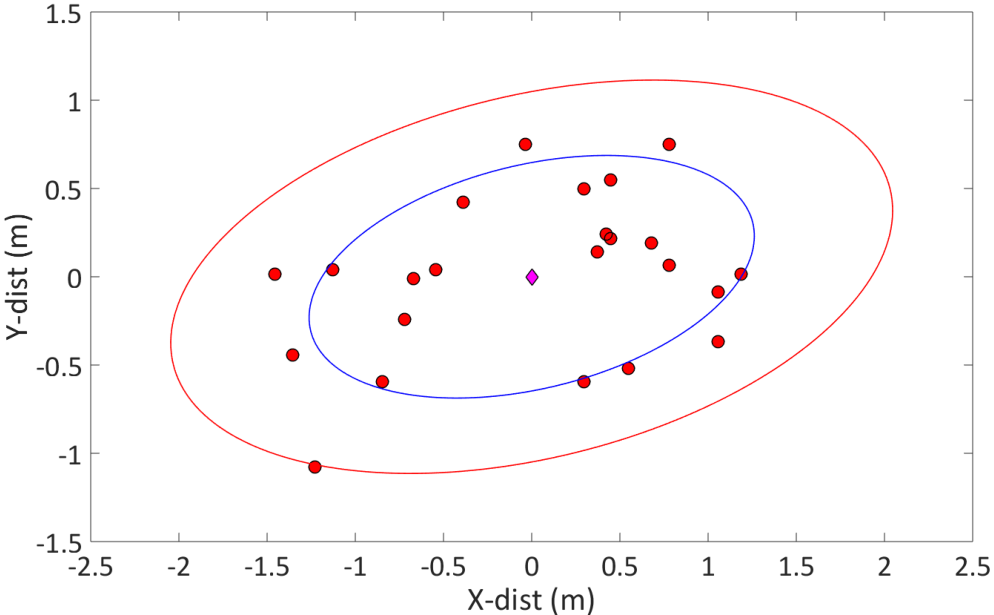
\includegraphics[width=\columnwidth]{SD_accu.pdf}}
 \caption{Targeting accuracy.  Circles show landing locations of 24 darts, each commanded to drop at the same GPS location. The mean position is marked by a diamond, ellipses show  $\sigma$ and 2$\sigma$ covariance.
 \label{fig:SD_accu.pdf}}
\end{figure}


\subsection{Height vs. penetration depth}
%Exp 5: Height vs. penetration depth

FAA rules require that UAVs fly below 400 feet (122 m). Our highest drop tests were from 25 m, and resulted in well-planted geophones on a compacted field with density 4 kg/cm$^2$. Harder soils may require faster impact velocity, so this section examines possible impact velocities as a function of drop height.
For ease of analysis, we will assume the SeismicDart has a constant coefficient of drag $C_d$ and that the drag force is proportional to velocity squared and equal to $\frac{1}{2} v^2 \rho A C_d$, where $v$ is the velocity, $A$ the cross-sectional area and $\rho$ the density of air.  
 The tests were performed near sea level, so $\rho \approx 1.225~\text{kg/m}^3$.
  The dart body is 0.06 m in diameter so $A=0.028$ m$^2$.  We will assume the dart $C_d$ is between that of a streamlined body $C_d=0.04$ and that of an arrow $C_d=1.5$~\cite{miyazaki2013aerodynamic}, and choose that of a sphere $C_d=0.47$.
The terminal velocity is then
\begin{align}
v_T = \sqrt{\frac{2 m g}{\rho A  C_d}} \approx 59 \text{ m/s.}
\end{align}
The velocity at impact is a function of the drop height $h$.
\begin{align}
v_{impact} = v_T  \sqrt{ 1 - e^{ -\frac{\rho A  C_d}{m} h }} \approx 59\sqrt{ 1 - e^{ -0.008 h }} \text{ m/s}
\end{align}
With  $C_d=0.47$, our drop from 25 m achieves only 43\% the terminal velocity (21.1 m/s), and for $C_d=0.04$ only 13\% terminal velocity  (22.0 m/s).
%This implies our tests are far from the limits of the SeismicDart's per
%This implies the SeismicDart is suitable even for much harder soils than tested thus far.
Dropping from the maximum FAA height of 122 m would generate an impact velocity of 39 m/s with $C_d=0.47$,  enabling penetration of harder soils.

\subsection{Robustness}
  The darts are robust. One of the darts used for the shot gather in Fig.~\ref{fig:shotgather_auto_drop} was a veteran of 120 drops.
The most damage observed occurred when we dropped a SeismicDart 10 m onto a bed of  rocks, each approximately  0.1 m in diameter. The steel spike of the dart was blunted, but this damage was quickly compensated by resharpening with a hand file and the SeismicDart was ready to redeploy.


%\begin{figure} \centering
%  {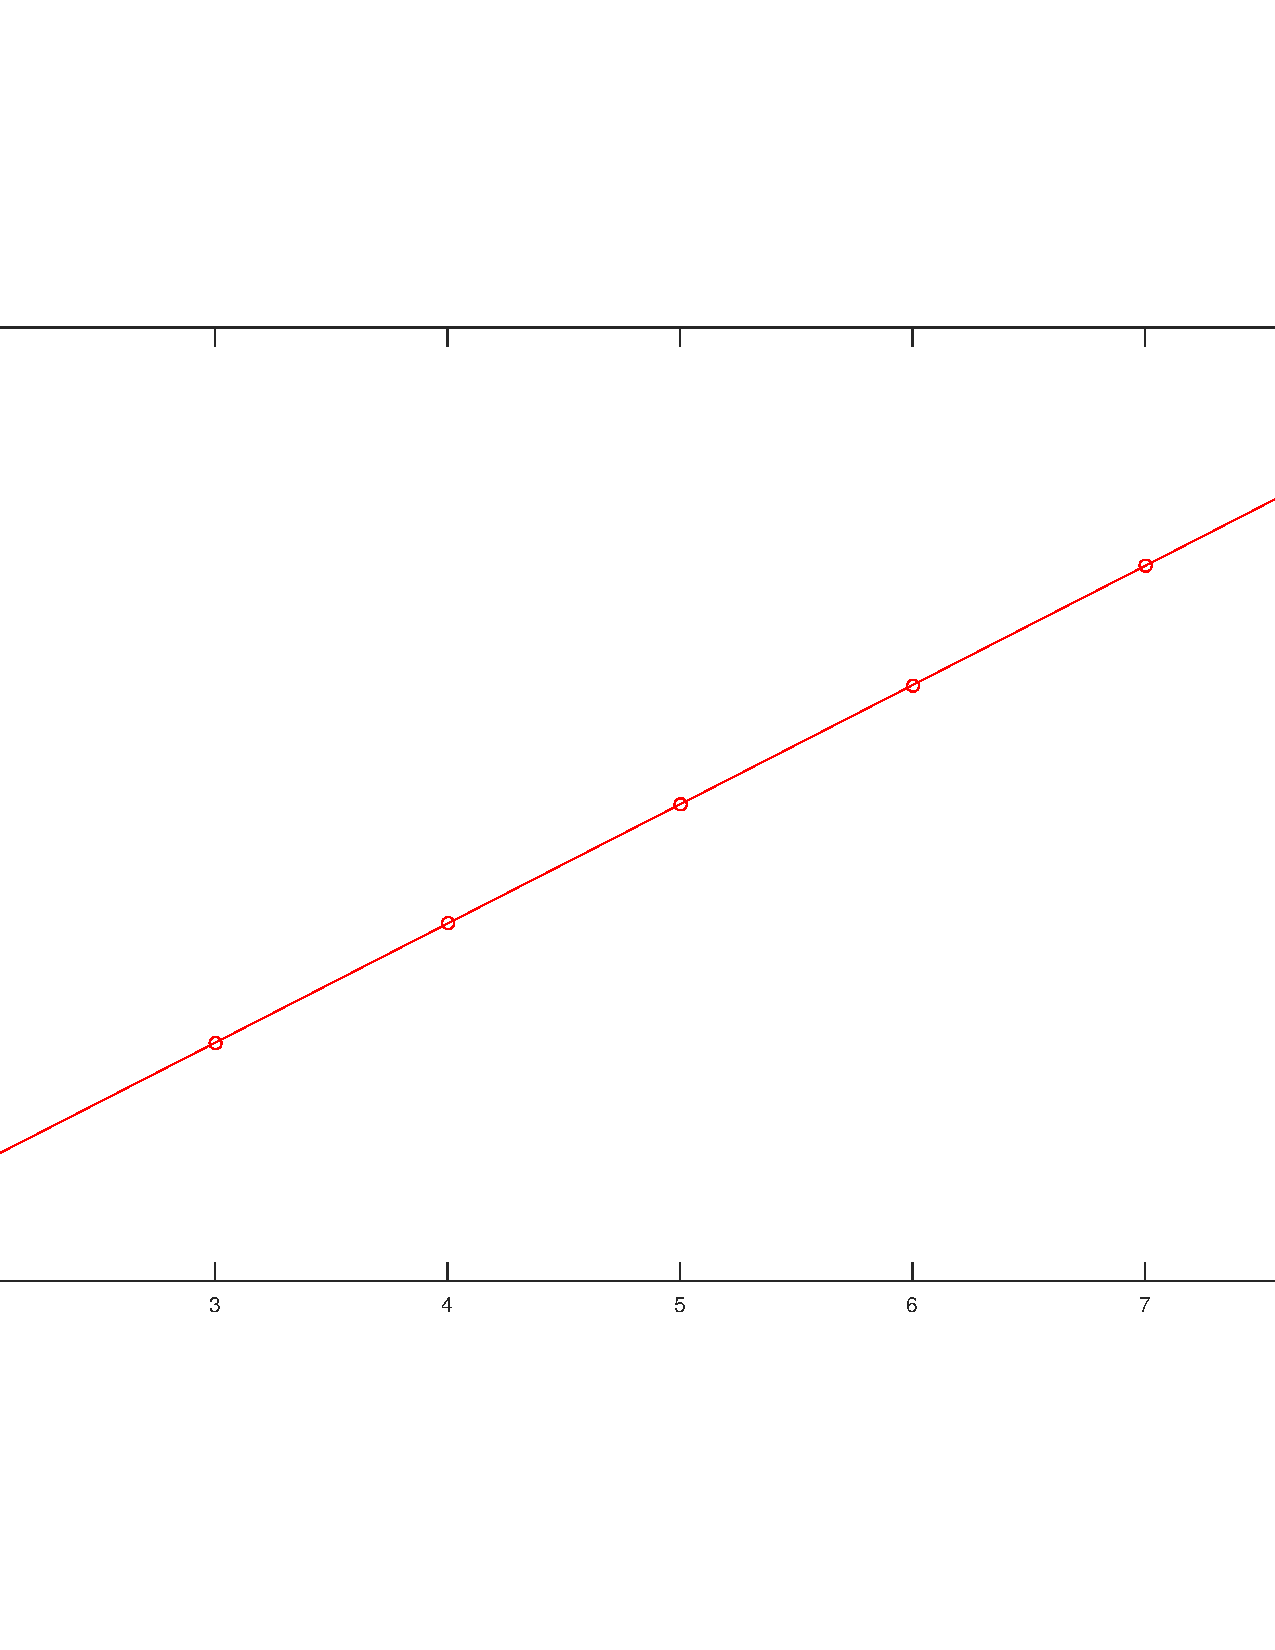
\includegraphics[width=\columnwidth]{replace_graph.pdf}}
% \caption{Plot of pneumatic cannon firing angle vs ending angle} 
% \label{fig:TradvsAutoDrop}
%\end{figure}






\section{Comparision}\label{sec:Comparision}


\begin{figure} \centering
  {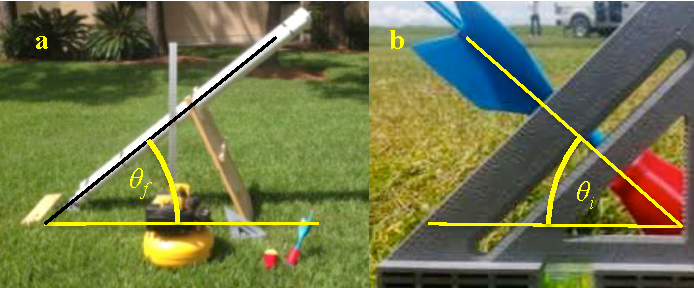
\includegraphics[width=\columnwidth]{CannonPicture}}
 \caption{A pneumatic launcher for SeismicDarts.  Ballistic dart deployment has limited usefulness because the incident angle is equal to the firing angle.} 
 \label{fig:CannonPicture}
\end{figure}

\begin{figure*}[htb]
\centering 
\vspace{1em}
\renewcommand{\figwid}{0.5\columnwidth}
\begin{overpic}[width =\figwid]{sim1_1.pdf}
\end{overpic}
\begin{overpic}[width =\figwid]{sim1_2.pdf}
\end{overpic}
\begin{overpic}[width =\figwid]{sim1_3.pdf}
\end{overpic}
\begin{overpic}[width =\figwid]{sim1_4.pdf}
\end{overpic}
\caption{Screenshots of simulations that were performed to estimate time take by different sensors surveying 100x100 m grid: a.) only SeismicSpiders b.) SeismicDarts and deployment system c.) heterogeneous system d.) human workers.
\label{fig:Sim_overview}}
\end{figure*}

\subsection{Ballistic Deployment}
To compare an alternative deployment mechanism we built the pneumatic cannon shown in Fig.~\ref{fig:CannonPicture}a.
The pneumatic cannon is U-shaped,  2 m in length, with a 0.1 m (4 inch) diameter pressure chamber and a 0.08 m (3 inch) diameter firing barrel, connected by an electronic valve (Rain Bird JTV/ASF 100). 
The cannon is aimed by selecting an appropriate firing angle $\theta_f$, azimuth angle, and chamber pressure.  
The reachable workspace is an annular ring whose radius $r$ is a function of the firing angle and initial velocity $v$. 
Neglecting air resistance, this range is found by integration:
\begin{align}
r = \frac{v^2}{g} \sin( 2 \theta_f )
\end{align} 
Initial velocity is limited by the maximum pressure and size of the pressure chamber.
The cannon used  SCH 40 PVC, which is limited to a maximum pressure of 3 Mpa (450 psi).

We charged our system to 1 Mpa (150 psi), and achieved a range of $\approx$ 150 m.
This range is considerably smaller than the UAV's range, which when loaded can complete a round trip of $\approx 1.5$ km.

A larger problem, illustrated in Fig.~\ref{fig:CannonPicture}, is that angle of incidence $\theta_i$ is equal to the firing angle $\theta_f$. 
Maximum range is achieved with $\theta_f = 45^\circ$, but this angle of incidence reduces the geophone sensitivity to $\cos(\theta_f )\approx 0.7$.
The placement accuracy of the cannon is lower than the UAV because a fired dart must fly over a longer distance than a dropped dart. 
Safety reasons also limit applications for a pneumatic launcher.





\begin{table} \centering
  {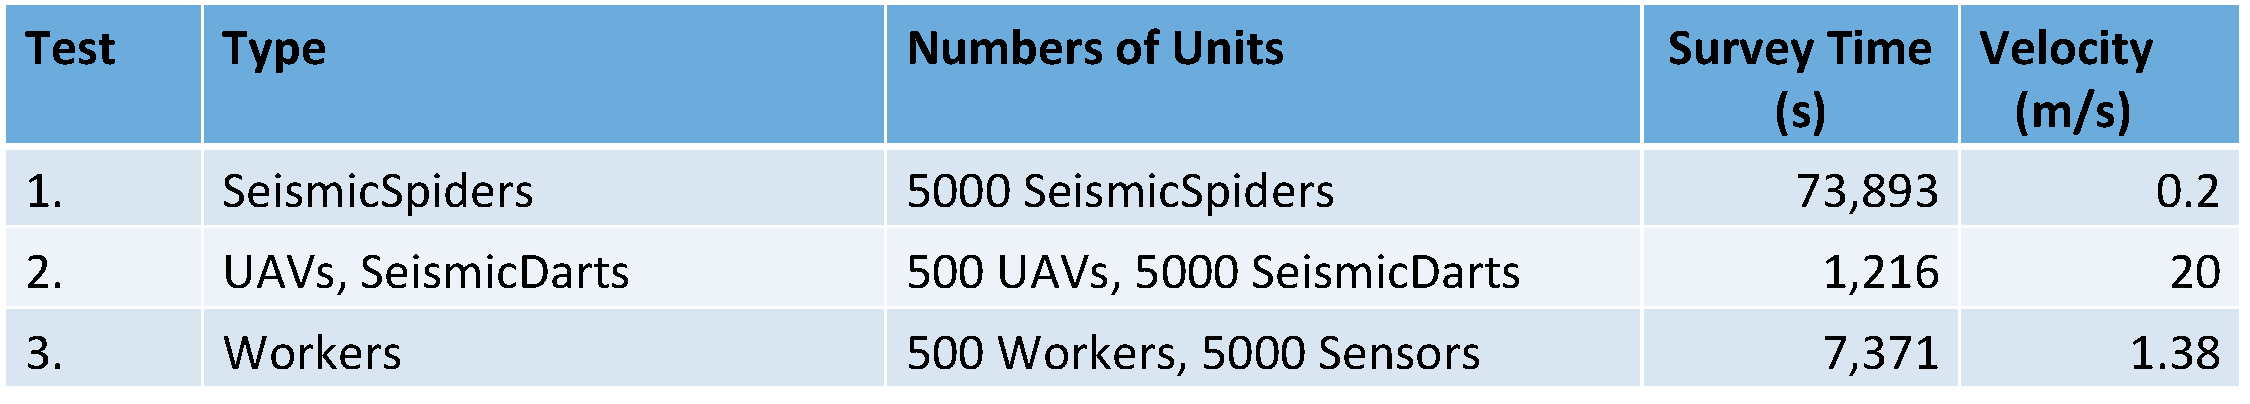
\includegraphics[width=\columnwidth]{simulation_table.pdf}}
 \caption{Comparison of different  deployment modes highlights the efficiency of UAV deployment.} 
 \label{tab:Sim_table}
\end{table}

\begin{figure} \centering
  {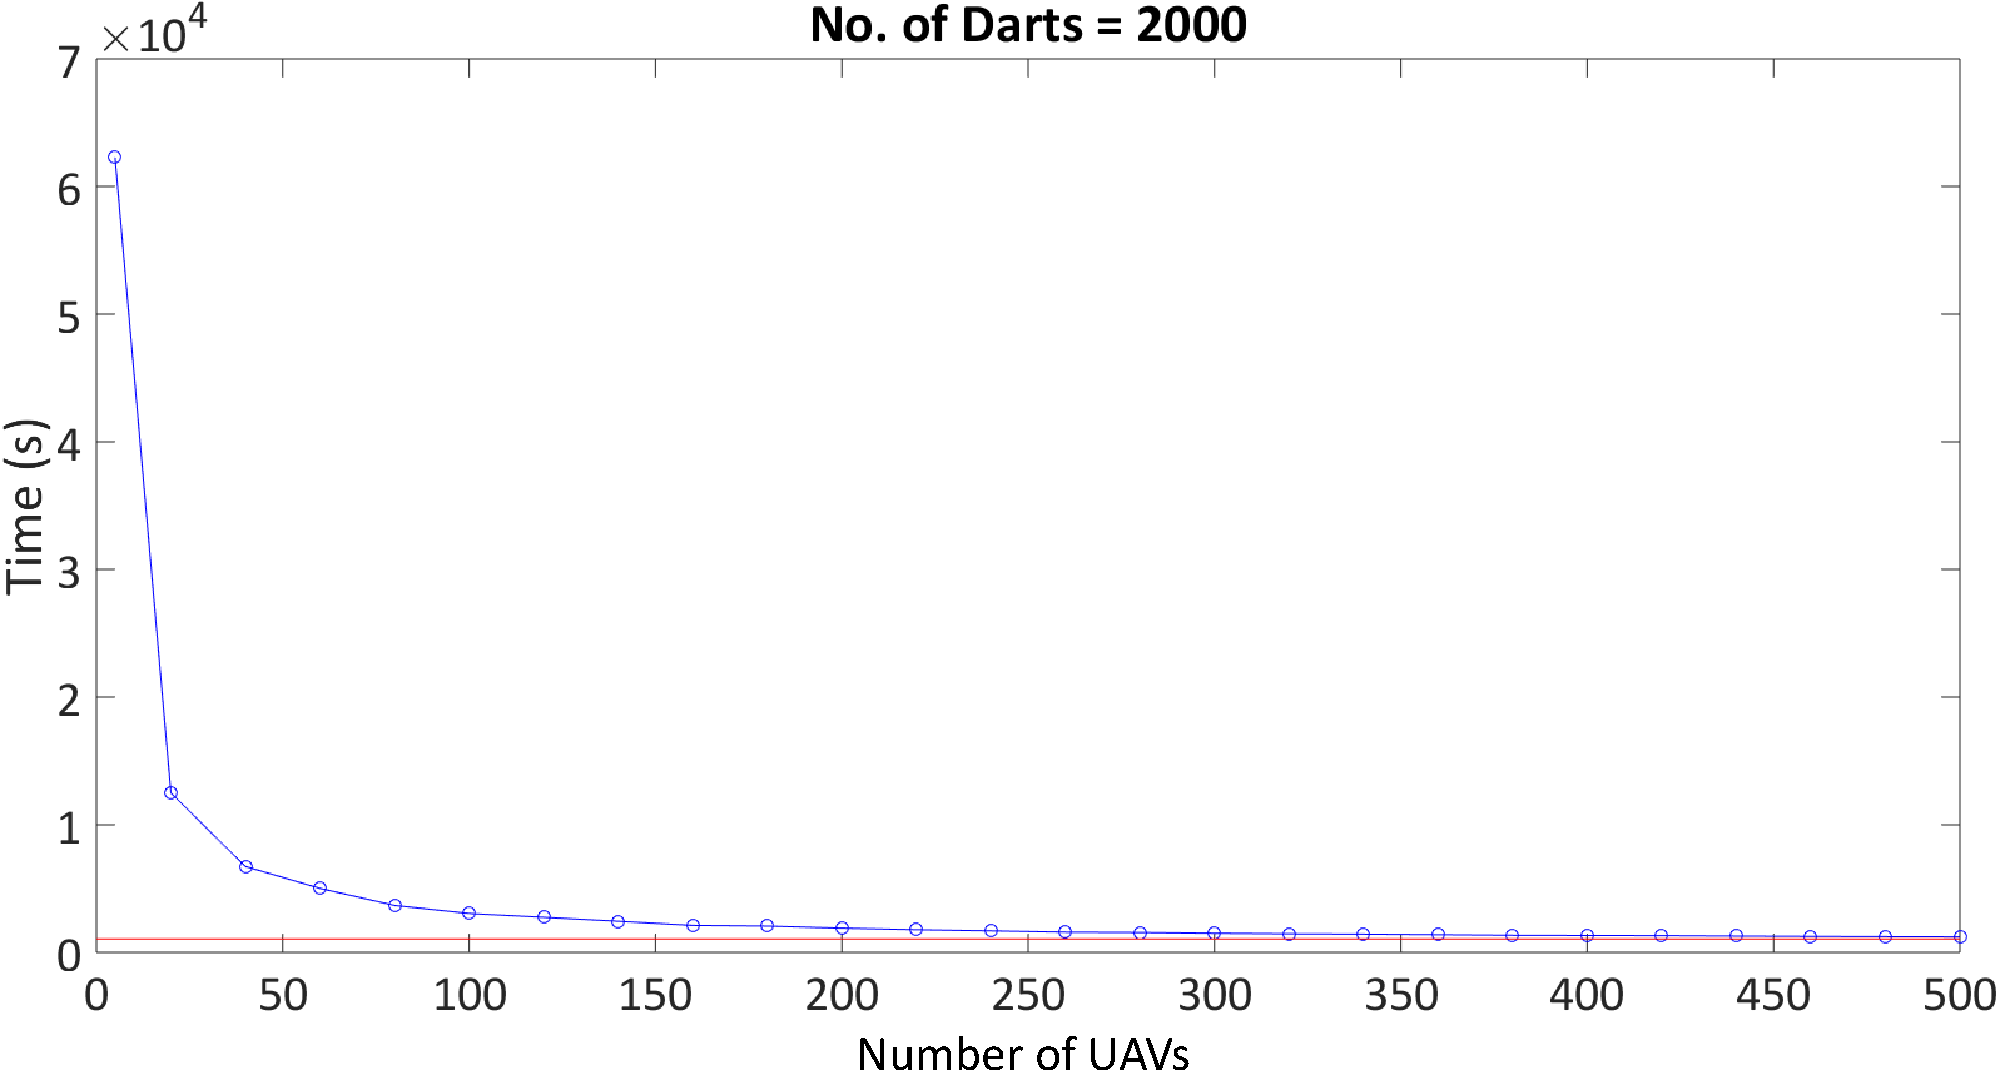
\includegraphics[width=\columnwidth]{DronevsTime.pdf}}
 \caption{Survey time for a 1km x 10 km region for different numbers of UAVs.} 
 \label{fig:DronevsTime}
 \vspace{-1em}
\end{figure}

\begin{figure} \centering
  {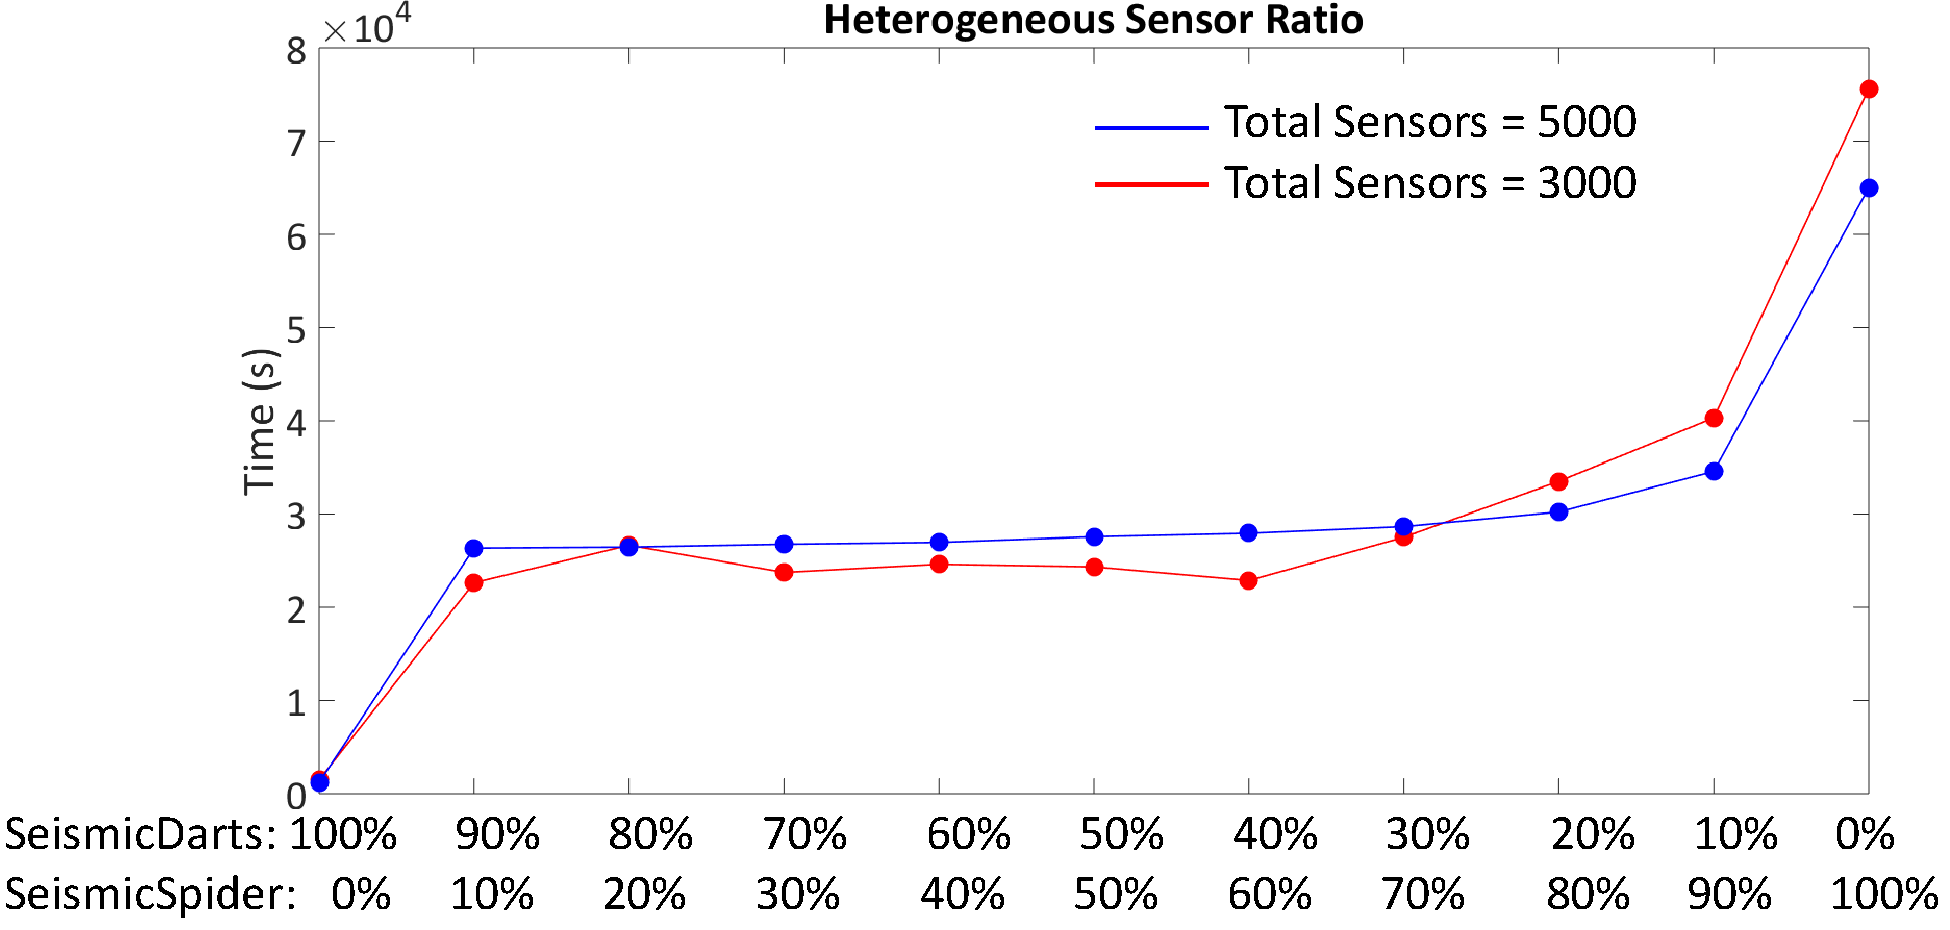
\includegraphics[width=\columnwidth]{het_sen_ratio.pdf}}
 \caption{Survey time for different sensor ratios. The total number of sensors \{5000, 3000\} were kept constant. Ten darts were provided for each UAV. } 
 \label{fig:het_sen_ratio}
  \vspace{-1em}
\end{figure}

\subsection{Simulation Studies}
   A scheduling system to compare  time and costs for seismic surveys with varying numbers of UAVs, SeismicSpiders, SeismicDarts, and human laborers was coded in  {\sc Matlab}, available at \cite{Srikanth2016seismicScheduler}.
% The goal of the Seismic Survey Scheduler is to estimate the requirements for a specific seismic survey. 
% The scheduler compare  time and costs for seismic surveys with varying numbers of UAVs, SeismicSpiders, SeismicDarts, and human laborers was coded in  {\sc Matlab}, available at \cite{Srikanth2016seismicScheduler}. 
   In each simulation, a seismic source must be measured at every survey point. 
   The scheduler must assign each sensor (SeismicDart or SeismicSpider) to an unmeasured survey point and assign each UAV or human worker a dart to pickup or deploy.  Once a sensor reaches a survey point, that sensor must wait until a seismic source is measured.
   A vibration truck (blue) provides the seismic source.
   Motion planning uses a centralized, greedy strategy.
   
   Frames from four different cases on a small survey region are shown in Fig.~\ref{fig:Sim_overview} on a 100x100 m area with survey points at 10 m spacing:
   a.) simulates 10 SeismicSpiders;  
   b.) simulates 5 SeismicUAVs deploying 50 SeismicDarts. Each UAV was allowed to carry up to 4 darts;
   c.) simulates 10 SeismicSpider, 5 SeismicUAVs and 50 SeismicDarts;
   d.) simulates 5 human workers deploying 75 SeismicDarts. Each worker was allowed to carry up to 10 darts. 
 Survey points are grey circles if unmeasured and green if measured.   The simulation uses red hexagons for SeismicSpiders,  black diamonds for UAVs,  inverted yellow triangles for SeismicDarts, and magenta diamonds for human workers. The assigned motion path for each sensor is colored magenta and the path completed is blue. 
 %The program simulates a seismic survey and records the time required. This allows comparing different combinations of sensing assets.

   
%  The first frame in Fig.~\ref{fig:Sim_overview} corresponds to SeismicSpiders (red hexagons) surveying a area of 100x100 m. 
%  Ten SeismicSpiders moving at a velocity of $0.1$m/s tries to visit each survey point (indicated by blue circles) on the map. 
%  Once ten of these sensors are at a new survey location the blue truck (Seismic source) perturbs the ground creating a seismic wave. The SeismicSpiders record the values at their current locations. 
%  Then they start moving to their next location and we repeat this process until we obtain readings at the survey locations. 
% % We follow a greedy approach to identify the SeismicSpiders new location.
%   The second frame in Fig.~\ref{fig:Sim_overview} corresponds to SeismicUAV (Black Diamond) deploying the SeismicDarts (inverted yellow triangle).
%    One SeismicUAV can carry four SeismicDarts simultaneously and drop them at different locations. 
%    Similar to the simulation involving the SeismicSpider once ten sensors are at a new survey point the blue truck takes a shot. 
%    The SeismicDarts record the readings at their corresponding locations.
%     Once this is done the SeismicUAV will pick up these SeismicDarts and redeploy them at new survey point.
%     % We follow a greedy approach to deploy these sensors. 
%      The third frame in Fig.~\ref{fig:Sim_overview} combines the SeismicSpider and SeismicDarts.
%       This represents a heterogeneous system surveying. 
%       The fourth frame in Fig.~\ref{fig:Sim_overview} represents human workers (magenta diamonds) servicing a region.
%        In all the simulations red lines connect the sensor location the sensor just surveyed to it's new location. 
%        The blue line connects the location the sensor just surveyed to it's current location. 
%        All sensors are assumed to start from the blue truck at $T = 0$. 
%        The Seismic Survey  simulates the proposed system and comparison with manual deployment could be achieved for analysis. 
%        The simulator is robust and all the parameters described above are variables. 
%        We want this tool to be used for preprocessing of a seismic survey in which you can vary the number of sensors, velocity, size of seismic survey, location of the seismic source etc.
%         Using this simulator we can closely match a real seismic survey and thus optimize the resources.
 

%A scheduling system to compare  time and costs for seismic surveys with varying numbers of UAVs, SeismicSpiders, SeismicDarts, and human laborers was coded in  {\sc Matlab}, available at \cite{Srikanth2016seismicScheduler}. Frames from four different cases are shown in Fig.~\ref{fig:Sim_overview}.

This tool allows us to examine engineering and logistic trade-offs quickly through simulations.  For example, Fig.~\ref{fig:DronevsTime} assumes a fixed number of darts and examines the finishing time with $5$ to $500$ UAVs.  The time required decays asymptotically, but $140$ UAVs requires only twice the amount of time required for $500$ UAVs, indicating  $140$ UAVs are sufficient for the task.    
 Substantial cost savings can be obtained by selecting the number of UAVs required to complete within a certain percentage greater than the optimal time.

The tool is useful for comparing the effectiveness of heterogeneous teams.  Table~\ref{tab:Sim_table} compares surveying a $1$ km x $10$ km strip of land with teams of (a) $5000$ SeismicSpiders, (b) $500$ UAVs and $5000$ SeismicDarts, (c) $500$ humans and $5000$ geophones.  Team (b) completed six times faster than team (c). 
  Since SeismicSpiders are  slower than UAVs and humans and are expensive compared to the SeismicDarts, their use is limited to special occasions. The UAV can deploy the SeismicSpider at a given waypoint. This attribute was not considered in the simulation but would improve deployment speed of SeismicSpiders.
   
In Fig.~\ref{fig:het_sen_ratio}, the total number of mobile agents are constant, but the percentage of UAVs and SeismicSpiders are varied.  10 SeismicDarts were provided for each UAV. Increasing the percentage of UAVs lowers the deployment time because UAVs move 20 m/s but SeismicSpiders move 0.2 m/s. 
The velocity difference makes UAV deployment time-efficient. 

\section[Conclusion]{Future Work}

This chapter presented a \emph{heterogeneous sensor system} and technique for autonomous geophone deployment.
The \emph{heterogeneous sensor system} compose of two components, UAV deployable SeismicDarts, mobile SeismicSpider.
The work in this chapter allow us to automate tasks that currently require a much more manual labors in hazardous environment.

The SeismicDart's output is comparable to well-planted geophones. 
For hard surfaces where the SeismicDart could not penetrate, we presented an autonomous alternative, the SeismicSpider.  
The SeismicSpider is mobile, can actively adjust its sensors to ensure ground contact and vertical placement, and can be deployed and retrieved by UAVs.

Autonomous deployment was conducted using GPS, proving human involvement could be minimized by adopting the proposed technique.
Hardware experiments compared the autonomous system to manual planting and ballistic deployment.
Simulation studies show time and cost savings over traditional manual techniques.

Future systems should be weatherized and optimized for cost, robustness, range, and speed.
Soil maps could be used to plan a survey, allocating SeismicSpiders to rocky or forested areas and SeismicDarts to penetrable soils.
These maps can be made more accurate using drone-carried ground penetrating radar \cite{merz2015new}.
Alternatively, the  SeismicDart's internal accelerometer also provides feedback on the quality of the plant.
As shown in Fig.~\ref{fig:AnglePlotIndoors}, angular deviations indicate a higher drop height is needed.

%
%
%\title{A Heterogeneous Robotics Team for Large-Scale Seismic Sensing} 
%%  compress using: gs -sDEVICE=pdfwrite -dCompatibilityLevel=1.4 -dNOPAUSE -dQUIET -dBATCH      -sOutputFile=RA-L2016compressed.pdf RA-L2016.pdf
%\documentclass[letterpaper, 10 pt, journal, twoside]{IEEEtran}
%\IEEEoverridecommandlockouts                              % This command is only needed if 
%                                                          % you want to use the \thanks command
%
%%\overrideIEEEmargins                                      % Needed to meet printer requirements.
%%\IEEEoverridecommandlockout
%%\documentclass[conference]{IEEEtran}
%\newcommand{\subparagraph}{}
%\usepackage{epsfig,graphicx,cite}
%\usepackage{psfrag}
%%\usepackage[small,compact]{titlesec}
%\usepackage{wrapfig}
%\usepackage{mathrsfs}
%\usepackage{bm}
%\usepackage{cite,url,subfigure,epsfig,graphicx}
%\usepackage{verbatim,amsfonts,amsmath,amssymb}
%\usepackage{fancyhdr}
%\usepackage{mathbbold}
%\usepackage{bbm}
%\usepackage{mathrsfs}
%\usepackage{amsfonts}
%\usepackage{cite,url,subfigure,epsfig,graphicx}
%\usepackage{amssymb,amsmath,bm,makecell}
%\usepackage{indentfirst}
%\usepackage{overpic}
%\newcommand{\figwid}{0.22\columnwidth}
%
%\usepackage{amsmath}
%\usepackage{algorithm}
%\usepackage[noend]{algpseudocode}
%
%\usepackage[T1]{fontenc}
%\usepackage[utf8]{inputenc}
%\usepackage{authblk}
%
%
%
%\usepackage{mathtools}
%\usepackage[font=footnotesize]{caption}
%\usepackage{amsmath}
%\usepackage{amssymb}
%\usepackage{tabulary}
%\usepackage{booktabs}
%\usepackage{framed}
%\usepackage{fancyhdr}
%%\usepackage[hypertex]{hyperref}
%\usepackage[hidelinks]{hyperref}
%%\IEEEoverridecommandlockouts
%\usepackage{cite,url,subfigure,epsfig,graphicx}
%\usepackage{times,verbatim,amsfonts,amsmath,color}
%%\newtheorem{definition}{\textbf{Definition}}
%%\newtheorem{lemma}{\textbf{Lemma}}
%%\newtheorem{proof}{\textbf{Proof}}
%%\newtheorem{theorem}{\textbf{Theorem}}
%%\newtheorem{example}{\textbf{Example}}
%%\newtheorem{proposition}{\textbf{Proposition}}
%%\newtheorem{remark}{\textbf{Remark}}
%%\newtheorem{corrolary}{\textbf{Corrolary}}
%%\newtheorem{ex}{\textbf{EX}}
%\usepackage{overpic}
%\graphicspath{{./},{./pictures/}}
%\setcounter{secnumdepth}{4}
%\setcounter{tocdepth}{4}
%\usepackage[table,xcdraw]{xcolor}
%\newcommand{\todo}[1]{ \textcolor{red}{\ttfamily#1}}
%\newcommand{\todobox}[1]{\vspace{5 mm}\par \noindent \framebox{\begin{minipage}[c]{0.98 \columnwidth} \ttfamily\flushleft \textcolor{red}{#1}\end{minipage}}\vspace{5 mm}\par}
%\let\labelindent\relax \usepackage{enumitem}
%
%
%
%
%
%\begin{document}
%%
%% paper title
%% can use linebreaks \\ within to get better formatting as desired
%\title{A Heterogeneous Robotics Team for Large-Scale Seismic Sensing} 
%% Paper headers
%\markboth{IEEE Robotics and Automation Letters. Preprint Version. Accepted Jan, 2017}
%{Sudarshan \MakeLowercase{\textit{et al.}}: Robotics Team for Seismic Sensing}
%% Use only for final RAL version
%
%\author{Srikanth K. V. Sudarshan$^{1}$,
%Victor Montano$^{1}$,
%An Nguyen$^{1}$,\\ 
%Michael McClimans$^{2}$,
%Li Chang$^{2}$,
%Robert R. Stewart$^{2}$, and
% Aaron T. Becker$^{1}$% <-this % stops a space
% \thanks{Manuscript received: September 10, 2016; Revised November 7, 2016; Accepted January 22, 2017.}%Use only for final RALversion
%\thanks{This paper was recommended for publication by Editor Roberts, Jonathan upon evaluation of the Associate Editor and Reviewers' comments. *This work was supported by the National Science Foundation under Grant No.\ \href{http://nsf.gov/awardsearch/showAward?AWD_ID=1553063}{ [IIS-1553063]}.}% <-this % stops a space
%\thanks{$^{1}$Department of Electrical and Computer Engineering,}
%\thanks{$^{2}$Department of Earth and Atmospheric Sciences,\\ University of Houston, 4800 Calhoun Rd, Houston, TX 77004, USA
%        {\tt\small \{skvenkatasudarshan, vjmontano, anguyen43, msmcclimans, lchang13, rrstewart, atbecker\}@uh.edu}}%
%\thanks{Digital Object Identifier (DOI): see top of this page.}
%}
%
%
%
%\maketitle
%%\thispagestyle{empty}
%%\pagestyle{empty}
%
%
%\begin{abstract} 
%Seismic surveying requires placing a large number of sensors (geophones) in a grid pattern, triggering a seismic event, and recording vibration readings. 
% The goal of the surveying is often to locate subsurface resources.  
%Traditional seismic surveying employs human laborers for sensor placement and retrieval. 
%The major drawbacks of surveying with human deployment are the high costs and time, and risks to humans due to explosives, terrain, and climatic conditions.
%We propose an autonomous, heterogeneous sensor deployment system using unmanned aerial vehicles (UAVs) to deploy mobile and immobile sensors.
%The proposed system begins to overcome some of the problems associated with traditional systems.  
%This paper provides detailed analysis and comparison with traditional survey techniques. 
%Hardware experiments and simulations show promise for automation reducing cost and time. 
% Autonomous aerial systems will have a substantial contribution to make in future seismic surveys. 
%\end{abstract}
%
%\begin{IEEEkeywords}
%	Aerial Robotics; Robotics in Hazardous Fields; Distributed Robot Systems
%\end{IEEEkeywords}
%
%\section{Introduction}\label{sec:Introduction}
% Drop letter for first word of the Introduction
% Here we have the typical use of a "T" for an initial drop letter
% and "HIS" in caps to complete the first word.
% \IEEEPARstart{T}{his} is the first sentence of my Introduction.
% Use only for final RAL version
\IEEEPARstart{s}{eismic} surveying is a geophysical technique involving sensor data collection and signal processing. 
%It aides in identifying hydrocarbon reservoirs such as petrol and natural gas. 
A primary application of the method is in the search for subsurface resources. 
Seismic methods are also used extensively in monitoring natural hazards such as earthquakes. 
Traditional seismic surveying requires manual laborers repeatedly placing geophone sensors at specific locations connected by cables. 
The cable length required is proportional to the area surveyed. 
Surveys routinely cover hundreds of square kilometers, requiring kilometers of cabling. 
Seismic surveying in remote locations is complicated by inaccessibility, harsh  conditions, and  transportation of bulky cables and sensors.  
These factors increase the cost. 

Nodal sensors, a relatively new development in seismic sensing, are autonomous units that do not require bulky cabling. 
They have an internal \emph{seismic recorder}, a micro-controller that records seismic readings from a high-precision accelerometer. 
Because this technology does not require cabling, downtime and overall cost can be reduced. 
However, these sensors are still planted and recovered by hand.  

\begin{figure}
\centering
\begin{overpic}[width=\columnwidth]{intro.pdf}\end{overpic}
\caption{\label{fig:Hetero_overall}
The heterogeneous sensor system presented in this paper: wireless SeismicDarts and a SeismicSpider, both designed for UAV deployment. 
}
\end{figure}

We propose a heterogeneous robotic system for obtaining seismic data, shown in Fig.~\ref{fig:Hetero_overall}. The system consists of two sensors, the SeismicDart and  the SeismicSpider.  
The SeismicDart is a dart-shaped wireless sensor that is planted in the ground when dropped  from an unmanned aerial vehicle (UAV). 
The SeismicSpider is a mobile hexapod with three legs replaced by geophones.
This system is designed to automate sensor deployment, minimizing cost and time while maximizing accuracy, repeatability, and efficiency.
  The technology presented may have wide applicability where quickly deploying sensor assets is essential, including geoscience research~\cite{werner2006deploying}, 
  earthquake~\cite{dominici2012micro} and volcano \cite{nagatani2013volcanic}  monitoring, defense operations~\cite{wu2007efficient}, and wildlife monitoring~\cite{dyo2010evolution,mainwaring2002wireless}. 
  
  
  
  

%%
%\section[Related Work]{Overview And Related Work}

This chapter presents a \emph{hetoerogenous seismic sensing system}, composed of stand alone geophone nodes deployed from unmanned aerial vehicles {UAV} and autonomous rovers with geophone attached.
We examine experimental data on geophone and soil coupling as a function of drop height and soil type.
We then provide a software tool for analyzing and planning a survey mission's logistic.
Our \emph{heterogenous sensor system} approach is designed to quickly and efficiently perform a survey with minimal manual labor for deployment and collection.

Sudarshan et al. \cite{sudarshan2015using} demonstrated a UAV equiped with four geophone sensors as landing gear.
The UAV in \cite{sudarshan2015using} can fly to a pre-programmed waypoint and land, attaching the geophones to the soil.

The geophones in  \cite{sudarshan2015using} had four problems:
(1) a UAV was required for each additional sensor,
(2) the force for planting the geophone was limited by the weight of the UAV,
(3) the platform required a level landing site,
(4) the magnets in the geophones distort compass readings, causing landing inaccuracy when autonomous.

The \emph{SeismicDart} presented in this system eliminates the need for a seperate UAV per sensor node.
Dropping the SeismicDarts from height also allows for greater penetration, firmer coupling and does not need a level landing site.
The new deployment unit also increase the distance between the SeismicDart's magnet and the UAV's magnetometer unit.

The SeismicSpider, our autonomous rover, can travel to survey locations inaccessible to UAV such as forests, thin atmosphere environments, caves or hard and rocky grounds which SeismicDarts cannot penetrate.
The SeismicSpider can also be deployed by a UAV, as close to the survey node as possible, then move to the desired location.

\subsection{Overview Of Seismic Sensing Theory}

\begin{figure}
	\centering
	\begin{overpic}[width=\columnwidth]{ral2016/Overview.pdf}\end{overpic}
	\caption{\label{fig:sensor_types}
	 Comparing state-of-the-art seismic survey sensors. a.) A traditional cabled system connects geophones in series to a seismic recorder and battery. b.) Autonomous nodal systems give each geophone a seismic recorder and battery.}
	%\vspace{-2em} 
\end{figure}



During seismic surveys, a source generates seismic waves that propagate under the earth's surface. 
These waves are sensed by geophone sensors and recorded for later analysis to detect the presence of resources. 
Fig.~\ref{fig:sensor_types} illustrates the components of current sensors. 

\subsubsection{Geophones}
Magnet-coil geophones contain a permanent magnet on a spring inside a coil. Voltage across the coil is proportional to velocity. 
 Beneath the coil housing is a metal spike. 
  Geophones are \emph{planted} by pushing this metal spike into the ground, which improves coupling with the ground to increase sensitivity. 
 The magnet-coil must be vertical. 
  Misalignment reduces the signal proportional to the cosine of the error.


\subsubsection{Cabled Systems}
Hydrocarbon exploration extensively uses traditional \emph{cabled systems} for seismic data acquisition.
Geophones are connected to each other in series using long cables. This cable is then connected to a seismic recorder and battery. 
The seismic recorder consists of a micro-controller which synchronizes the data acquired with a GPS signal and stores the data onboard. 
This method of data acquisition requires many manual laborers and a substantial expenditure for transporting the cables. 
Rugged terrain makes carrying and placing cables labor intensive, and the local manual labor pool may be unskilled or expensive.
   
\subsubsection{Autonomous Nodal Systems}
\emph{Autonomous nodal systems}~\cite{wood1998distributed} are now being used to conduct seismic surveys.
Unlike traditional cabled systems, autonomous nodal systems are not connected using cables.
The sensor, seismic recorder, and battery are all combined into a single package called a \emph{node} that can autonomously record data as shown in Fig.~\ref{fig:sensor_types}.
Even in these systems the data is generally stored in the onboard memory and can only be acquired after completing the survey.
This delay means errors cannot be detected and rectified while conducting the survey. 
Wireless autonomous nodes are a recent development.
These systems can transmit data wirelessly in real time~\cite{jiang2015geophysical}.
However, these systems still require manual laborers for planting the autonomous nodes at specific locations and deploying the large antennas necessary for wireless communication.
 
\subsection{Related Work}

Seismic surveying is a large industry.
The concept of using robots to place seismic sensors dates to the 1980s, when mobile robots placed seismic sensors on the moon~\cite{LSisMSE81}.
\cite{DSSMaA14} and \cite{coste2013seismic} proposed using a mobile robot for terrestrial geophone placement.
Plans are underway for a swarm of seismic sensors for Mars exploration~\cite{MAPL2006}.
Additionally,~\cite{muyzert2015marine} and~\cite{postel2014drone} proposed marine robots for hydrophone deployment underwater. 
Other work  focuses on data collection, using a UAV to wirelessly collect data from multiple sensors~\cite{wilcox2013seismic}.
Autonomous sensor deployment and mobile wireless sensor networks were studied in~\cite{howard2002mobile,corke2004autonomous,tuna2014autonomous}.
Heterogeneous mobile robotic teams were used for mapping and tracking in~\cite{howard2006experiments}.

%%
%\section[SeismicDarts]{SeismicDarts}

A SeismicDart combines a geophone (GS-100) with the fins and body of a lawn Jart\textsuperscript{TM}, using a 3D-printed chamber that encloses a WiFi-enabled microcontroller (particle.io Photon\textsuperscript{TM}) as shown in Fig.~\ref{fig:Smart_Dart_overview}. 
The center of the chamber is slotted to fit a wooden plate holding an accelerometer that transmits data wirelessly through the microcontroller. 
The centered accelerometer card allows placing the microcontroller and battery on opposite sides, balancing the dart.
Designs and instructions to build a SeismicDart are available at \cite{Victor2016Thingiverse}.



\begin{figure} \centering
{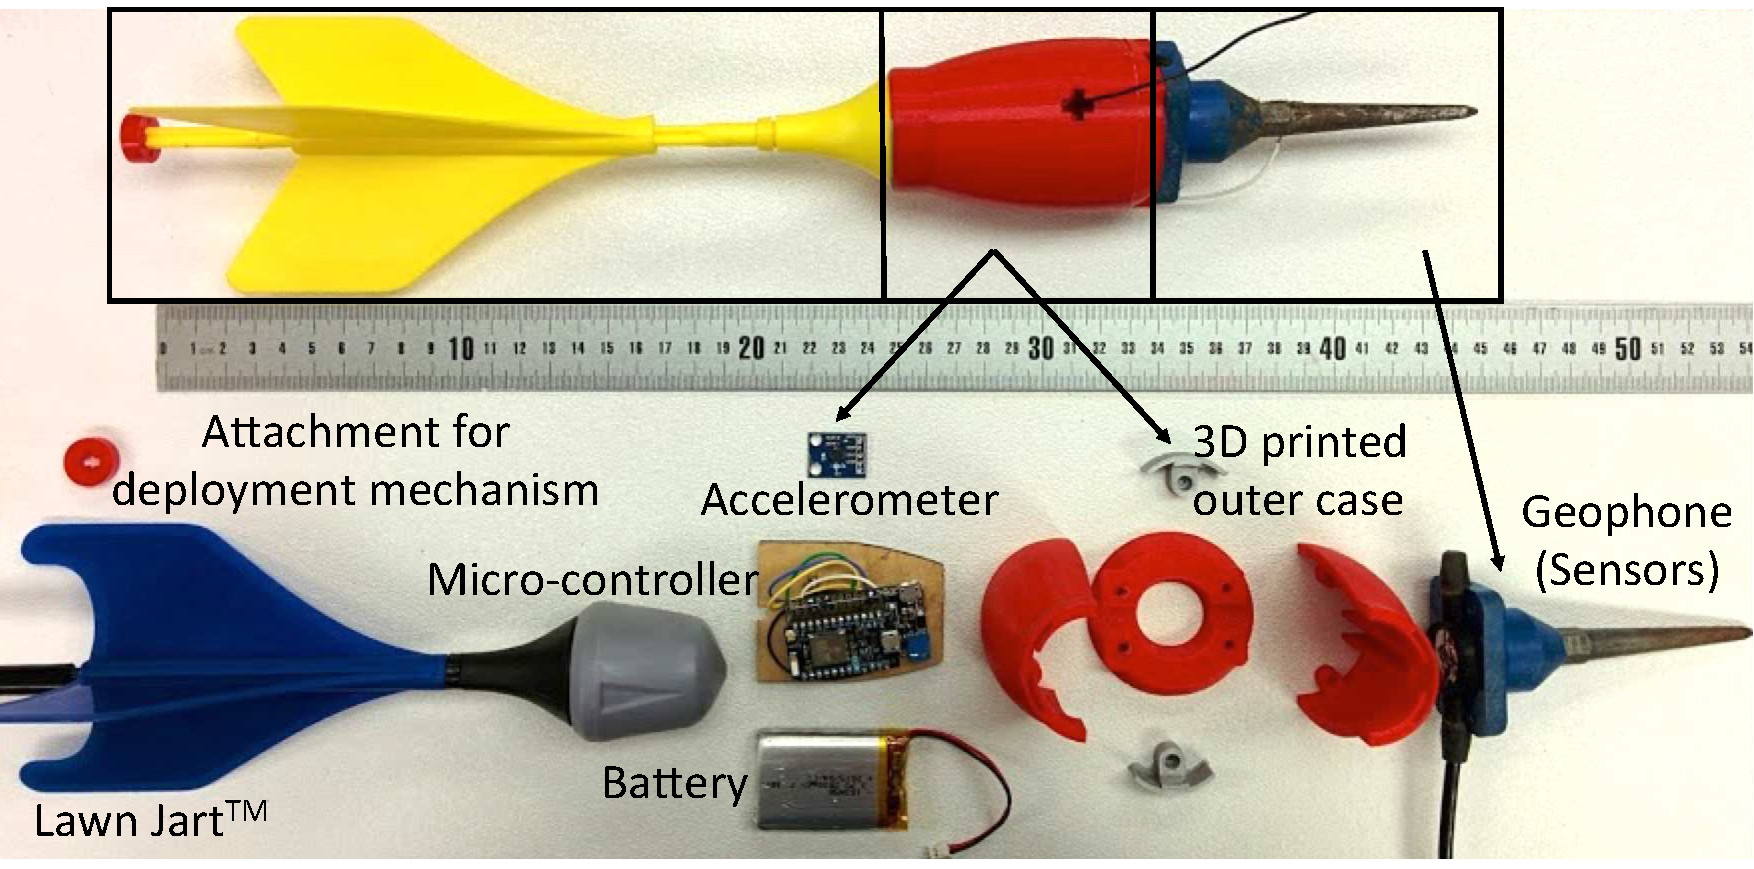
\includegraphics[width=\columnwidth]{ral2016/Smart_Dart_overview.pdf}}
\caption{Components of the SeismicDart sensor: a lawn  Jart\textsuperscript{TM} fin, particle.io Photon\textsuperscript{TM}  micro-controller, 3D printed protective casing, and a geophone.} 
\label{fig:Smart_Dart_overview}
\end{figure}

%%%%%%%%%%%%%%%%%%%%%%%%%%%%%%%%%%%%%%% 
\subsection{Experiments} 
The following sections compare SeismicDart performance.
\subsubsection{ Drop tests in different soils}  


Proper planting of a geophone requires good contact with the soil and the geophone to be in a vertical position. 
Geophone protocol classifies a geophone as well planted if the angle of deviation is less than 10$^\circ$ and the spike has at least 40 mm of penetration.

To determine how SeismicDarts perform in different soils, this experiment measured penetration depth and angle of deviation in seven different soil types as a function of drop height. 
 The soil types were categorized by compression strength, in kg/cm$^2$, measured using a soil pocket penetrometer (CertifiedMTP). Measurements for compression strength vary with a small deviation in measurement location, so we repeated this measurement 10 times at 10 different locations in each soil type and computed the average.
 
 Experiments were conducted using the UAV to autonomously drop a payload of four SeismicDarts at the desired drop height. 
 Tests were conducted at drop heights of 10, 15, 20, and 25 m. 
 We measured the angle of deviation and penetration depth for each drop.
 The angular deviation was measured using two protractors.
 We measured penetration depth by marking where the spike met the soil, pulling the dart from the soil, and measuring the distance from the spike tip to the marking with calipers. 
  We repeated this measurement 12 times for each soil type at each drop height.  The soil compression strengths in these experiments ranged from 0.056 kg/cm$^2$ for river sand, to 4 kg/cm$^2$ for a hard-packed soccer field.

Because the four soil types with the lowest soil compression strength could be well-planted with low drop heights, we performed these tests manually. 
We filled 19 liter (5 gal.) buckets with four soil types and dropped the SeismicDart from six heights.
%Penetration depth and angular deviation were measured. %To measure penetration depth, the buried darts were marked where the spike met the soil, the dart was then pulled from the soil, and the distance from the spike tip to the marking was measured with calipers. The angular deviation was recorded using the accelerometer inside the dart.

 
  % These experiments shows that increasing drop height increases penetration on all soils tested.
  % Also, darts dropped in quiescent air remain vertical if they penetrate the soil.
Experiment results plotting penetration depth as a function of drop height are displayed in Fig.~\ref{fig:DepthPlotIndoors}, and angle of deviation as a function of drop height in Fig.~\ref{fig:AnglePlotIndoors}.   Both graphs are annotated with values for soil compression strength. 

\begin{figure} \centering
{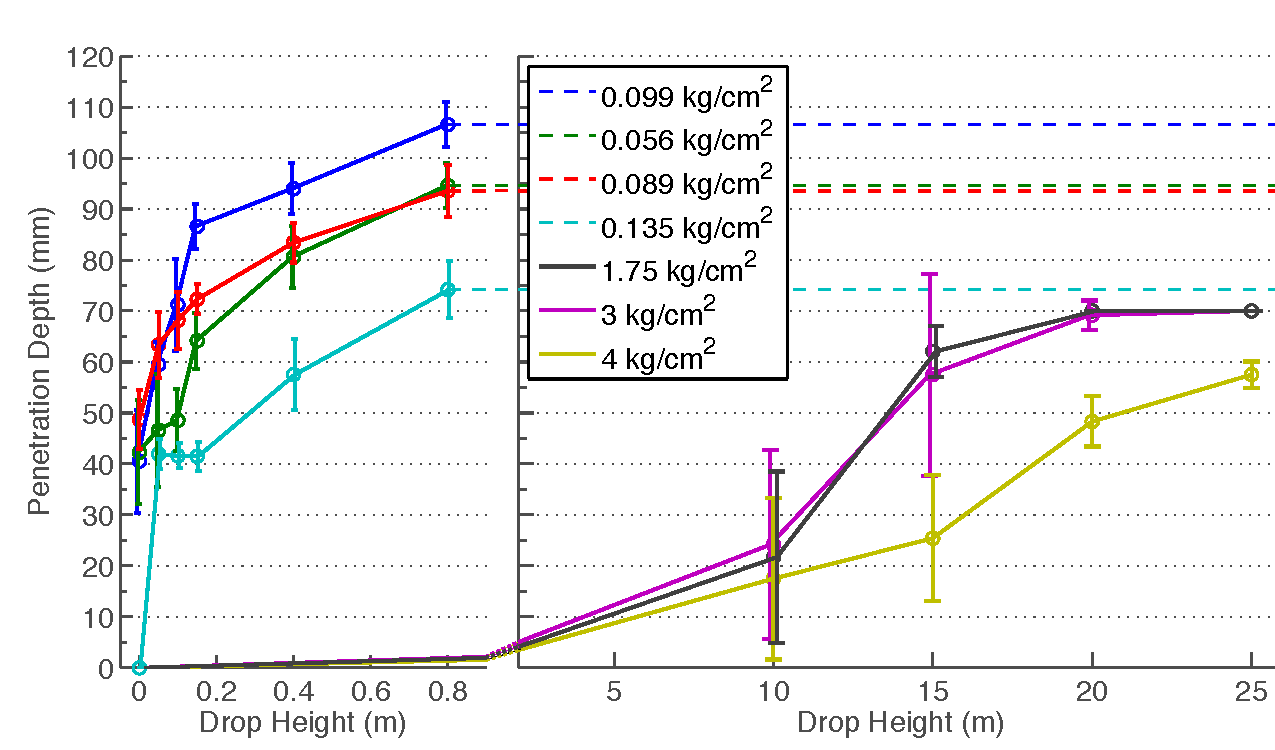
\includegraphics[width=\columnwidth]{ral2016/AutoPenetrationDepth2.pdf}}
\caption{Drop height vs. penetration depth in seven soil types. Drops were performed autonomously and each data point represents 12 trials. Increasing the drop height increased the penetration depth for all seven soil types.} 
\label{fig:DepthPlotIndoors}
\end{figure}

\begin{figure} \centering
{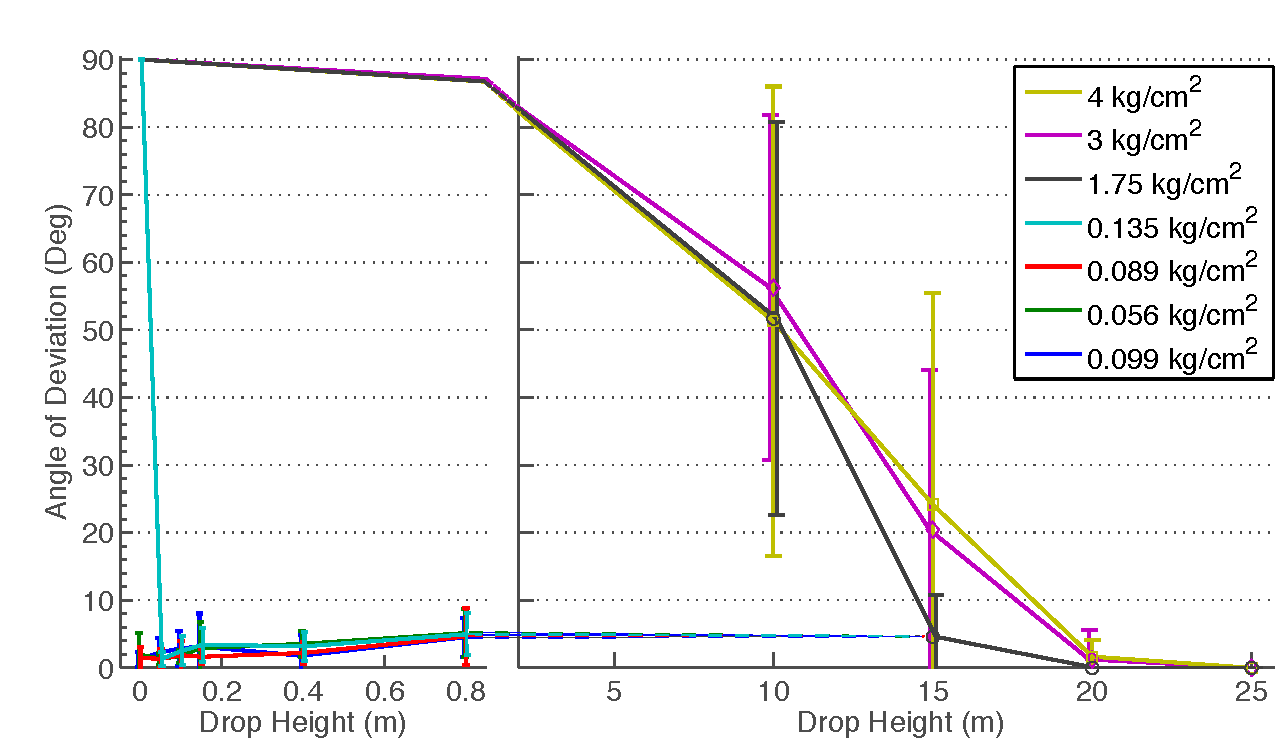
\includegraphics[width=\columnwidth]{ral2016/AutoPenetrationAngle2.pdf}}
\caption{Drop height vs. angle of deviation in seven soil types. Drops were performed autonomously and each data point represents 12 trials. Increasing the drop height reduced the angle of deviation for all seven soil types.} 
\label{fig:AnglePlotIndoors}
\vspace{-1em}
\end{figure}

If a SeismicDart is dropped from a sufficient height into penetrable soil, the spike will be buried into the soil and the geophone will have a small angular deviation from vertical. Soils with higher compression strength require higher drop heights. Error bars show that variance decreases with drop height for angle of deviation and penetration depth.  
 All drops from heights 20 m or more achieved the goals of an angle of deviation less than 10$^\circ$ and at least 40 mm of penetration.   

The autonomous tests were conducted with 16 km/hr winds, demonstrating that drop heights 20 m or higher were sufficient to counter disturbances from the wind. %https://www.windfinder.com/forecast/galveston_airport

\subsubsection{Shot gather comparison} 
Geophysical explorationists often use thousands of geophones to conduct a seismic survey. 
 As a proof-of-concept, this experiment ran a small-scale seismic survey to compare the performance of a traditional cabled four geophone system with readings from four autonomously deployed SeismicDarts.
Flying autonomously at a drop height of 25 m, the UAV flew to GPS waypoints spaced 4 m apart and deployed one dart at each location. 
A seismic survey technician manually planted four traditional cabled geophones, each 10 cm from a deployed SeismicDart. 
A seismic wave was generated using a sledgehammer hitting a steel plate.

Results of the field test comparison between the traditional cabled geophone system and the SeismicDarts are shown in Fig.~\ref{fig:shotgather_auto_drop}.   
Data were obtained using a \emph{StrataVisor}, a device that can obtain, store, and plot the sensed data. 
The \emph{StrataVisor} is extensively used with traditional geophone setups because the geophones can only sense vibrational waves and are dependent on other devices for storage and data processing. 
To allow a fair comparison with geophones, the SeismicDart's  ability to store sensed data was not used in this experiment. 
 The \emph{StrataVisor} records the geophone voltage at 2000 Hz, using a 24 bit ADC.

The readings from both systems are qualitatively similar, with no discernible phase or amplitude differences. Let $X$ be measurements from the traditional geophone and $Y$ the corresponding voltages from a SmartDart.
The percent peak-to-peak error and normalized root-mean-square error (NRMSE) are defined as
\begin{align}
e_{pp} &= 100 \left( \frac{ \max(X) - \min(X) }{ \max(Y) - \min(Y) } -1\right) \\
  \text{NRMSE} &=\frac{100}{\max(X) - \min(X)} \sqrt{ \frac{ \sum_{i=1}^n \left( X_i - Y_i \right)}{n} }.
\end{align}
The peak-to-peak errors were [-6.33, -1.15, -1.81,  9.84] \% for sensors at [4,8,12,16] m from the source.
 The NRMSE were [1.05,1.27,3.98,4.39] \% for sensors at [4,8,12,16] m from the source.
%$e_{\text{4 m}}  =  -6.3 \%, e_{\text{8 m}}  =  11.93 \%, e_{\text{12 m}}  = -1.81\%, e_{\text{16 m}}  = 0.981 \%$. 
%The RMSD error were $RMSD_{\text{4 m}}  =  -6.3 \%, RMSD_{\text{8 m}}  =  11.93 \%, RMSD_{\text{12 m}}  = \%, RMSD_{\text{16 m}}  = 0.981 \%$. 
Readings were also compared using a Pearson product-moment correlation coefficient, which gives a correlation measurement between $-1$ and $+1$ where $+1$ is total positive linear correlation:
\begin{align}
\rho_{X,Y} = \frac{E\left[  (X-\mu_X) (Y-\mu_Y)  \right]}{  \sigma_X, \sigma_Y}.
\end{align}

The correlation coefficients were $\rho_{\text{4 m}}  =  0.9813, \rho_{\text{8 m}}  =  0.9836, \rho_{\text{12 m}}  =  0.8600, \rho_{\text{16 m}}  = 0.8114$. These correlations decrease with distance. The SeismicDart is subject to low-amplitude noise, which is easiest to see in the fourth sensor because it was 16 m from the seismic source and thus had the lowest signal amplitude.  This noise is potentially due to wind striking the SeismicDart's fin. The effect of noise can be mitigated by using larger seismic sources such as a vibration truck or explosives.



\begin{figure} \centering
  {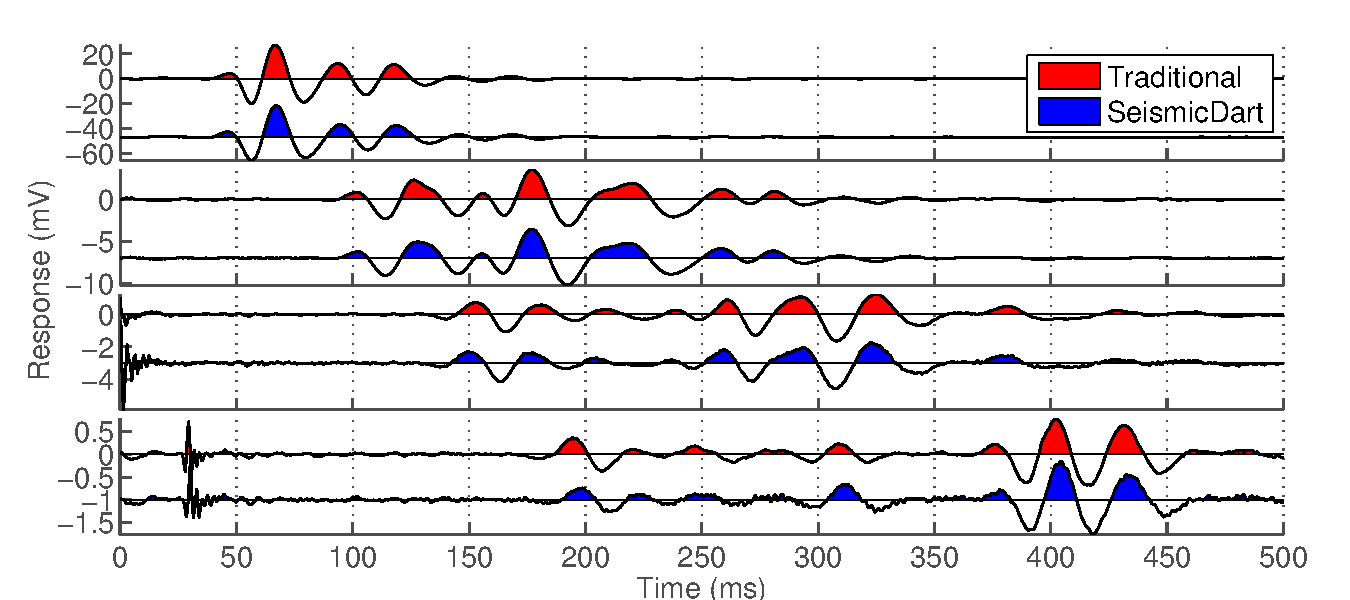
\includegraphics[width=\columnwidth]{ral2016/SeismicSurveyComparison.pdf}}
 \caption{Raw voltage data from shot gather comparison of four traditional geophones and four autonomously dropped SeismicDart sensors.  
 \label{fig:shotgather_auto_drop}}
\end{figure}

\subsection{SeismicDart Deployment and Retrieval}
First, the SeismicDarts are loaded onto to a UAV. 
Currently, a maximum of four sensors can be dropped in a single flight. 
The flight plan communicated to the UAV provides a GPS waypoint for each SmartDart. 
The UAV flies to and drops a SmartDart at each waypoint, then returns home. 

Deployment is only one part of a survey. Large surveys require moving and reusing sensors.  
Because SmartDarts are more expensive than standard geophones, rapid reuse is essential.
The UAV has an underslung hook for picking up a SeismicDart.
Retrieval is facilitated by attaching a wire loop to the SeismicDart tail.
 This loop provides a target 300 mm in diameter for the hook, yet still allows autonomous deployment, as shown in Fig.~\ref{fig:SeismicDart_DR}.
Currently, retrieval is performed by manually piloting the UAV, but the loop size is within the accuracy of a UAV equipped with RTK GPS.
%Automating retrieval is out of the scope of this paper.



\begin{figure} \centering
  {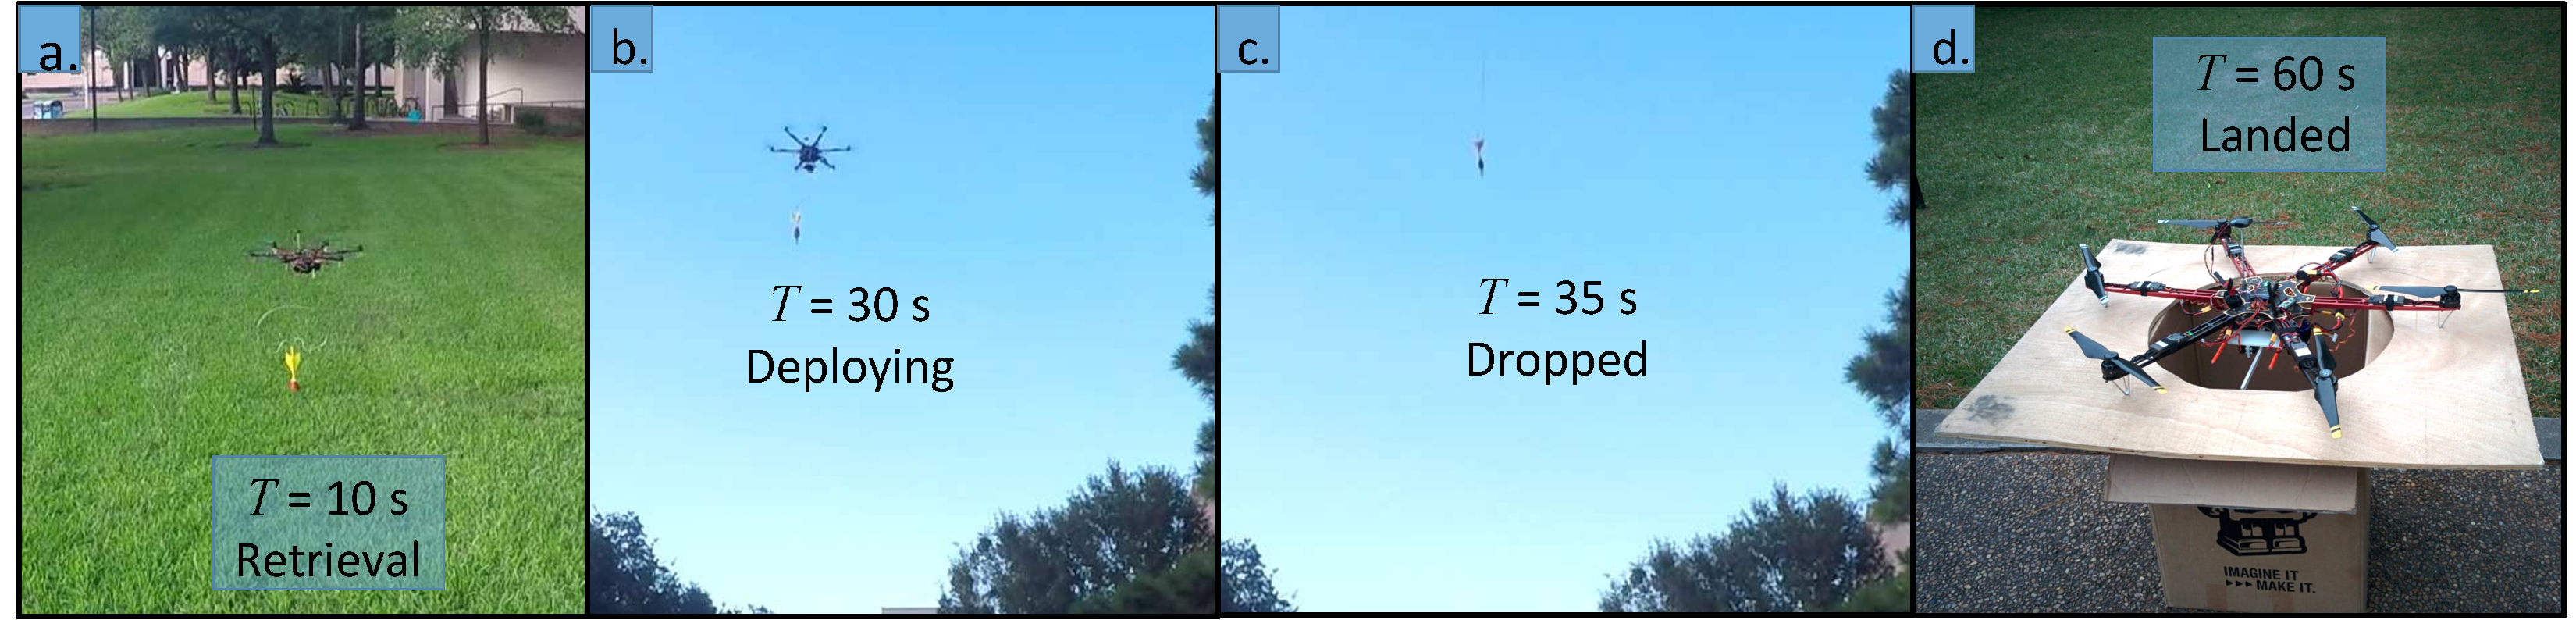
\includegraphics[width=\columnwidth]{ral2016/SeismicDart_DR.pdf}}
 \caption{SmartDart retrieval and redeployment.  See video attachment. 
 \label{fig:SeismicDart_DR}}
\end{figure}
 

%%
%\section{SeismicSpider}\label{sec:SeismicSpider}


\begin{figure} \centering
  {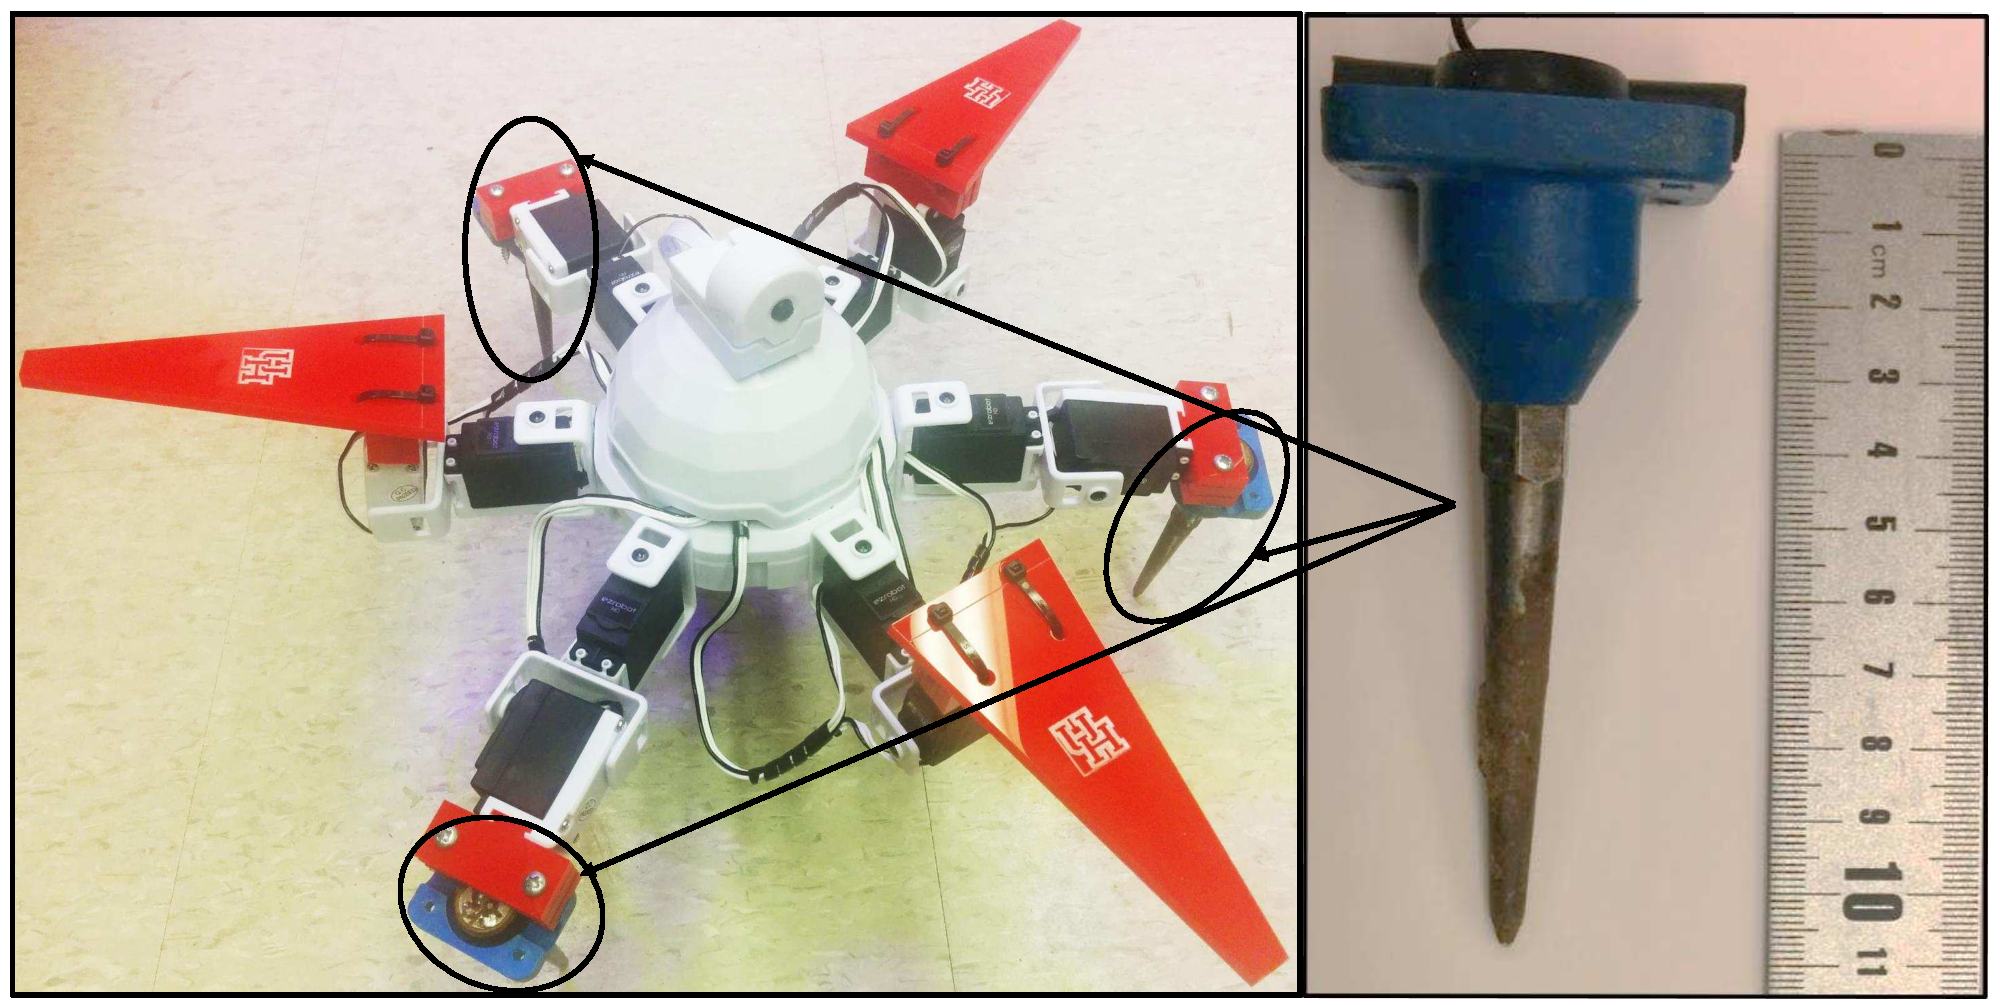
\includegraphics[width=\columnwidth]{Hex_overview.pdf}}
 \caption{The SeismicSpider is a six-legged mobile robot where geophones replace three legs. It is drone deployable, can sense and record seismic data, and can move to desired locations, including terrain the SeismicDart cannot access.} 
 \label{fig:Hex_overview}
\end{figure}


The SeismicSpider, shown in Fig.~\ref{fig:Hex_overview}, is built from the Six Hexapod kit designed by EZ-Robots. Each of the six legs is powered by two 15 kg$\cdot$cm lever servos. Three legs were replaced by three GS-20DM 14 Hz geophones from Geospace Technologies. The remaining three legs were designed to match the geophone dimensions.

 Our initial plan to use three geophones required the spider to raise the three inactive legs while acquiring data. This lack of support caused excessive strain on the three servo motors responsible for holding the spider upright, introducing unwanted vibration into the system.  Positioning the geophone legs at 20$^\circ$ to normal enhances stability and relieves the excessive stress on the servos. 
 The three geophones were in series, so with each geophone leg angled inward, superposition replicates the signal from one vertical geophone.
 
 Traditional geophones are mounted in an insulated, shock-resistive enclosure on a spike. The spikes, varying in length, are inserted into the ground to ensure a firm coupling with the environment. The design of our SeismicSpider prevents full depth insertion of the 88 mm spikes. 

	To overcome the coupling issue we are using three geophones per station compared to the typical one. Our immediate goals were to compare amplitude response to that of a standard single station.	
 

\subsection{Shot gather comparison}
%\subsubsection{Accuracy plot}
%Hexapod move to desired GPS location  (plot accuracy)\\
%\subsubsection{ Shot gather comparison}

A line of twenty-four geophones (GS-20DM 14 Hz) were laid out at one-meter intervals with our inline source seven meters from the nearest geophone. Beginning from the farthest offset of 31 m we manually aligned the Spider with the corresponding geophone, fired the source, then moved one meter ahead. 

%\paragraph{Results}
Data from the shot gather comparison is shown in Fig.~\ref{fig:shotgatherHexpod}.
The response for three geophones in series was 5 dB greater than a single geophone. The geophone wires proved insufficient to insulate against 60 Hz noise. Hence the raw data from the traditional setup as well as the SeismicSpider was processed with a (3-50) band-pass filter. Finally, the SeismicSpider data was attenuated by $-5$dB to level the comparison.    

\begin{figure} \centering
  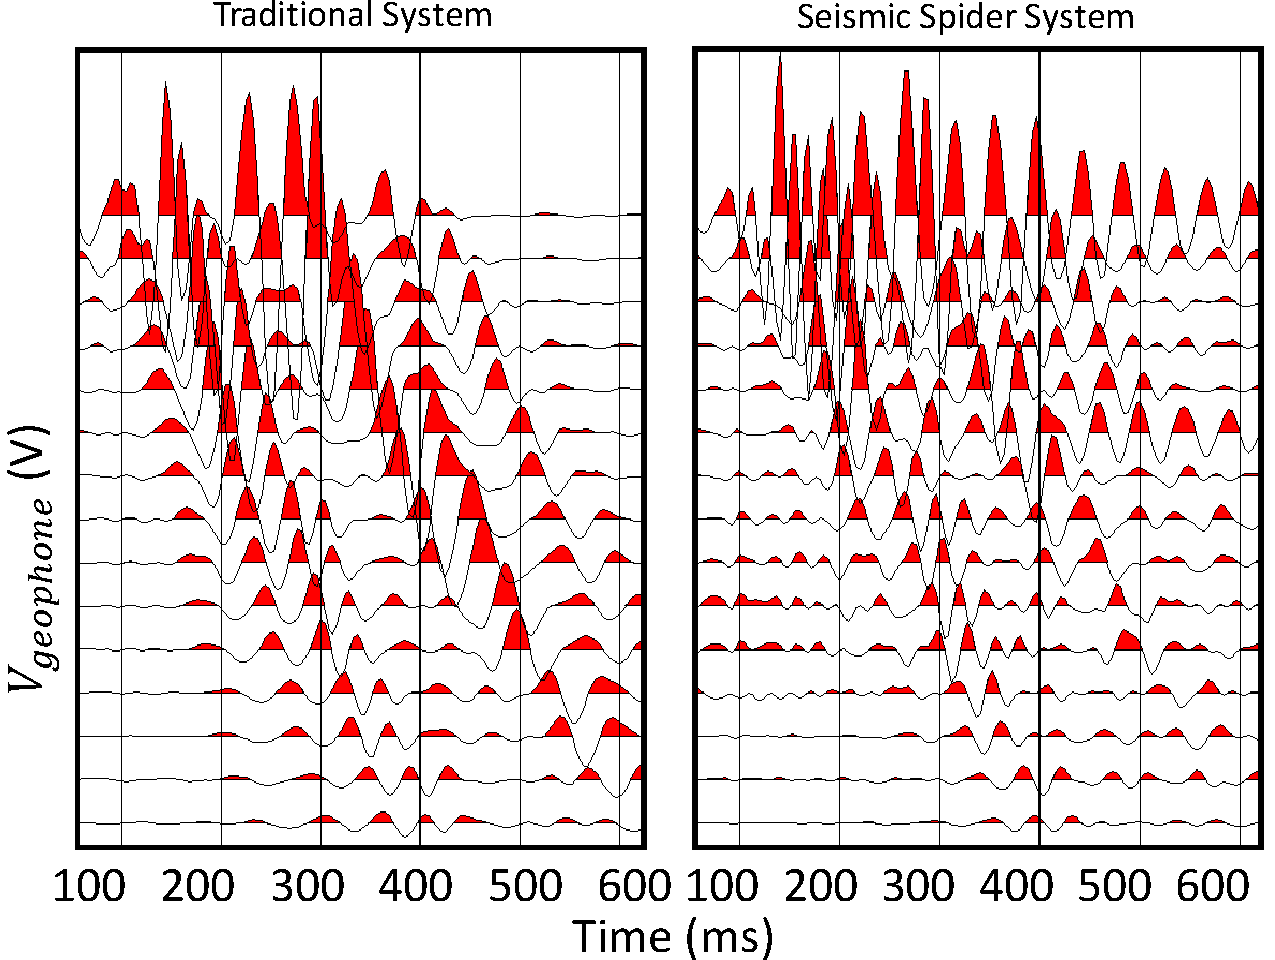
\includegraphics[width=\columnwidth]{shotgather_hex.pdf}
 \caption{Shot gather comparison of traditional geophones vs. SeismicSpider. 
 \label{fig:shotgatherHexpod}}
\end{figure}

%\paragraph{Future work}	we must filter 60 Hz noise, compare adding geophones to all six legs, and design a larger seismic survey to ensure adequate data for phase analysis. Design improvements could be done to make the SeismicSpider an active sensor.   


\subsection{Deploying and Retrieving the SeismicSpider}

\begin{figure} \centering
  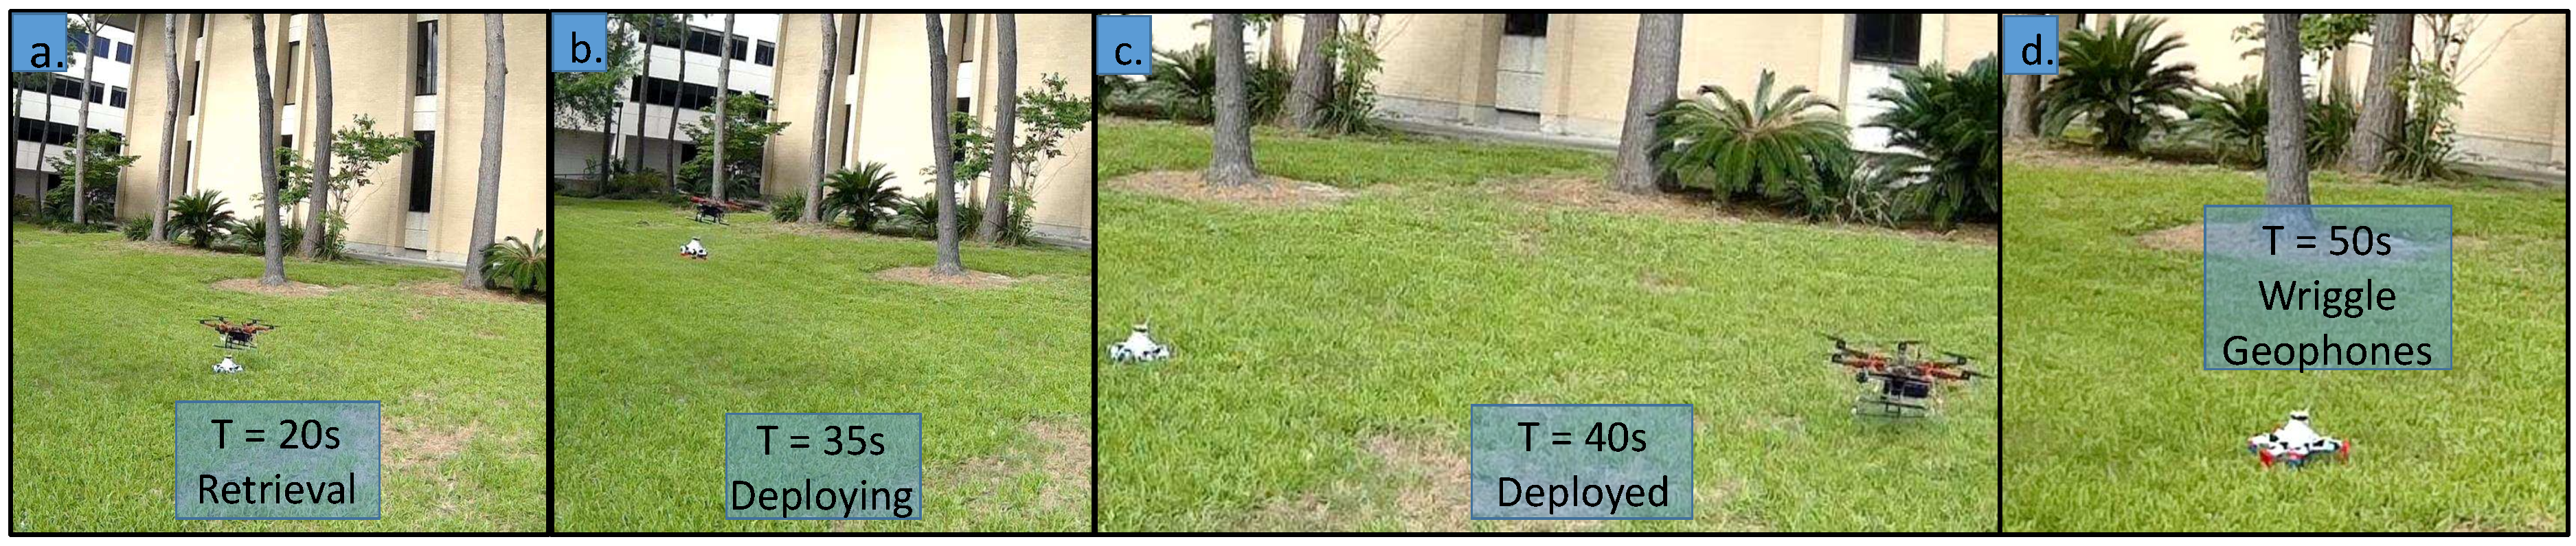
\includegraphics[width=\columnwidth]{SeismicSpider_DR.pdf}
 \caption{SeismicSpider retrieval and redeployment. See video attachment. 
 \label{fig:SeismicSpiderDR}}
\end{figure}

The UAV's purpose is to deploy sensors at desired GPS waypoint locations. The SeismicSpider is a mobile robot, but it is substantially slower than the UAV.  The UAV carrying the SeismicSpider flew autonomously to a programmed waypoint. The deployment mechanism included a hook controlled by a servo attached to the UAV. The UAV lowered to a waypoint 0.5 m from the ground, then the servo was triggered to unhook the SeismicSpider.  The SeismicSpider was then wirelessly powered on. 
The SeismicSpider also has an onboard GPS, enabling it to navigate to desired waypoints. 
After walking to the sensing location, the SeismicSpider was programmed to shake its three non-sensing legs to plant its geophone legs into the ground.  
  Currently, autonomous deployment of sensors is implemented, but the retrieval is piloted. 
Combining the mobility of the SeismicSpider with the speed of the UAV enables reaching locations inaccessible by air or impossible to penetrate by SmartDarts.
Fig.~\ref{fig:SeismicSpiderDR} shows the SeismicSpider being retrieved and then redeployed by a UAV.






%%
%\section{UAV and deployment unit}\label{sec:DeploymentUnit(UAV)}

The UAV is a custom-built, 1.77 m wingspan hexacopter, controlled by a Pixhawk flight controller running ArduPilot Mega flight software. The UAV has a 3DR GPS module using the UBlox NEO-7 chipset.


 The deployment mechanism allows the UAV to carry four SeismicDarts in a circular array, and release them when it reaches the desired GPS location, one at a time.
 The rear of the dart has a circular tip that locks into the deployment mechanism, and rests on a rectangular slot-path. 
 A servomotor rotates the dart tips through the rectangular slot-path, allowing darts to release from a circular opening,  as shown in Fig.~\ref{fig:deployment_system}.



\begin{figure} \centering
  {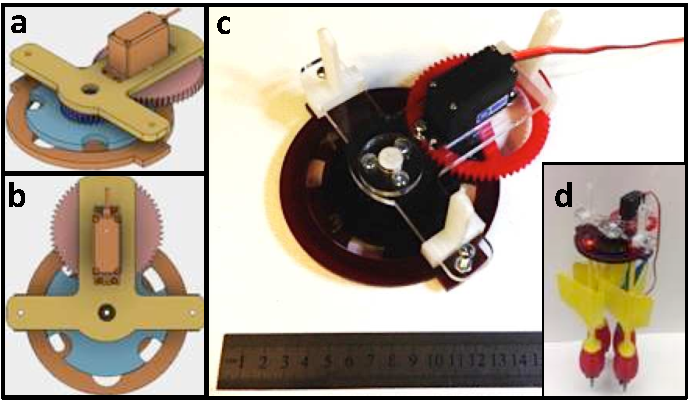
\includegraphics[width=\columnwidth]{deployment_system.pdf}}
 \caption{Deployment system for dropping SeismicDarts from the UAV. Pictured design holds four darts, but can be scaled according to the UAV's carrying capacity.} 
 \label{fig:deployment_system}
\end{figure}




\subsection{Autonomous drop demonstration and accuracy}

The current UAV can place a SeismicDart within $\pm1$ m of the desired location.  
This range is within tolerances for seismic surveys because often features (rocks, water, etc.) exist that require this amount of error from theoretically assigned locations and some survey designs include a random placement component to improve noise cancellation.
%(3) this error minimally perturbs the data since seismic waves travel at 600 m/s near the surface, so a one-meter inaccuracy equates to $\approx$1.6 ms delay.
%(4) the response of a receiver to seismic vibrations is an average over a number of meters.  ?? what does this mean??

To accurately perform a seismic survey, the sensors do not need to placed accurately, but their position must be known within $\approx$ 0.01 m. 
 Knowledge of the exact location compensates for placement inaccuracy.
 Localization can be achieved by placing an RTK GPS in each dart.  A lower-cost solution would use an RTK GPS on the SeismicDrone and perform image registration with the downward facing camera.  As shown in the multimedia attachment, even at a 25 m drop height a planted dart occupies dozens of pixels, enabling cm-level localization accuracy.


%allows corrections for jitter in signal arrival times due to  placement inaccuracy.


%Exp 4: Automatic drop from drone, accuracy in placement
\begin{figure} \centering
  {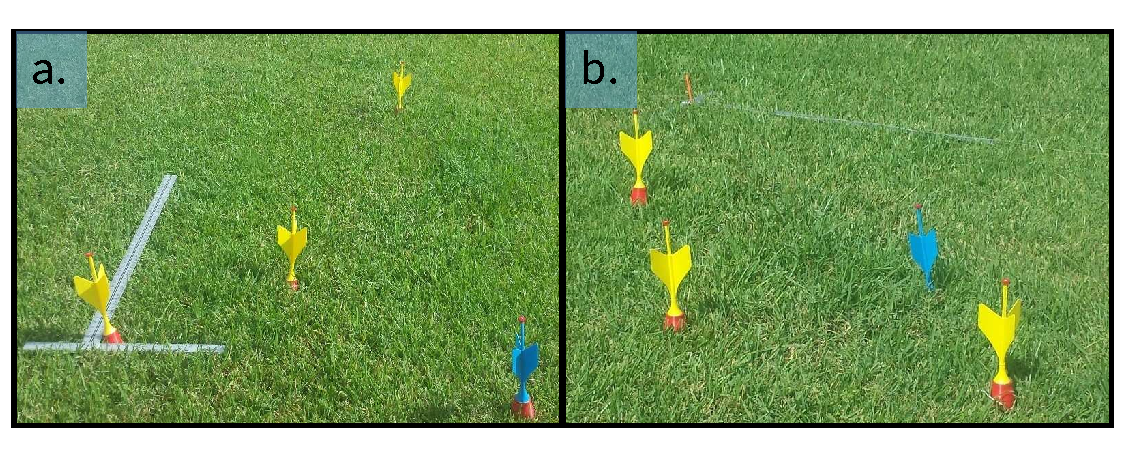
\includegraphics[width=\columnwidth]{accuracy_test_overview.pdf}}
 \caption{a.) First set of darts with reference axes. b.) Third dart set. } 
 \label{fig:Accu_test_darts}
\end{figure}

For the accuracy test, six sets of darts, four darts in each set, were dropped on the same GPS waypoint. Between each drop, the UAV traveled to a nearby GPS waypoint to cancel out the flight controller's stable hover.
The UAV then returned to the launch platform to be reloaded, we recorded the dart landing positions, collected the darts, and reloaded the darts on the UAV for the next deployment set.
The measurement method of the darts' positions are shown in Fig.~\ref{fig:Accu_test_darts}.
Results are shown in Fig.~\ref{fig:SD_accu.pdf}.
  
%To measure position, one dart was picked from the first set as the reference point (the lower left in Fig.~\ref{fig:Accu_test_darts}b), hence the first data point was (0,0). A 1-m T-square was placed with the origin at the dart's drop point to establish reference axes.


 %A rod was placed in the position of the first dart to keep reference as shown in Fig.~\ref{fig:Accu_test_darts}c. 
% The T-square was kept in place and mason twine was suspended to lengthen the reference axes. 
% Future deployments were measured  using the reference point and axes. 



\begin{figure} \centering
  {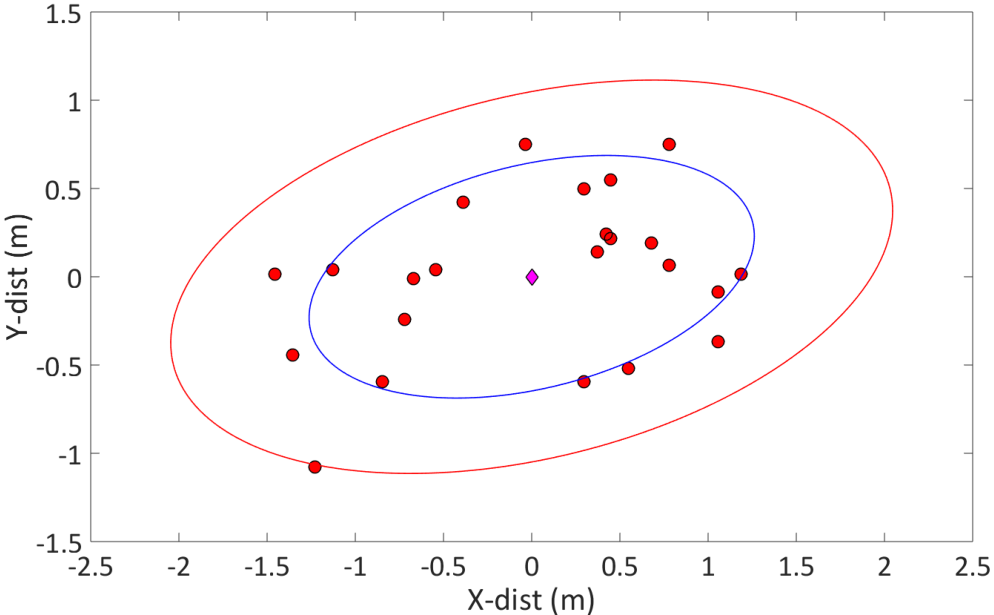
\includegraphics[width=\columnwidth]{SD_accu.pdf}}
 \caption{Targeting accuracy.  Circles show landing locations of 24 darts, each commanded to drop at the same GPS location. The mean position is marked by a diamond, ellipses show  $\sigma$ and 2$\sigma$ covariance.
 \label{fig:SD_accu.pdf}}
\end{figure}


\subsection{Height vs. penetration depth}
%Exp 5: Height vs. penetration depth

FAA rules require that UAVs fly below 400 feet (122 m). Our highest drop tests were from 25 m, and resulted in well-planted geophones on a compacted field with density 4 kg/cm$^2$. Harder soils may require faster impact velocity, so this section examines possible impact velocities as a function of drop height.
For ease of analysis, we will assume the SeismicDart has a constant coefficient of drag $C_d$ and that the drag force is proportional to velocity squared and equal to $\frac{1}{2} v^2 \rho A C_d$, where $v$ is the velocity, $A$ the cross-sectional area and $\rho$ the density of air.  
 The tests were performed near sea level, so $\rho \approx 1.225~\text{kg/m}^3$.
  The dart body is 0.06 m in diameter so $A=0.028$ m$^2$.  We will assume the dart $C_d$ is between that of a streamlined body $C_d=0.04$ and that of an arrow $C_d=1.5$~\cite{miyazaki2013aerodynamic}, and choose that of a sphere $C_d=0.47$.
The terminal velocity is then
\begin{align}
v_T = \sqrt{\frac{2 m g}{\rho A  C_d}} \approx 59 \text{ m/s.}
\end{align}
The velocity at impact is a function of the drop height $h$.
\begin{align}
v_{impact} = v_T  \sqrt{ 1 - e^{ -\frac{\rho A  C_d}{m} h }} \approx 59\sqrt{ 1 - e^{ -0.008 h }} \text{ m/s}
\end{align}
With  $C_d=0.47$, our drop from 25 m achieves only 43\% the terminal velocity (21.1 m/s), and for $C_d=0.04$ only 13\% terminal velocity  (22.0 m/s).
%This implies our tests are far from the limits of the SeismicDart's per
%This implies the SeismicDart is suitable even for much harder soils than tested thus far.
Dropping from the maximum FAA height of 122 m would generate an impact velocity of 39 m/s with $C_d=0.47$,  enabling penetration of harder soils.

\subsection{Robustness}
  The darts are robust. One of the darts used for the shot gather in Fig.~\ref{fig:shotgather_auto_drop} was a veteran of 120 drops.
The most damage observed occurred when we dropped a SeismicDart 10 m onto a bed of  rocks, each approximately  0.1 m in diameter. The steel spike of the dart was blunted, but this damage was quickly compensated by resharpening with a hand file and the SeismicDart was ready to redeploy.


%\begin{figure} \centering
%  {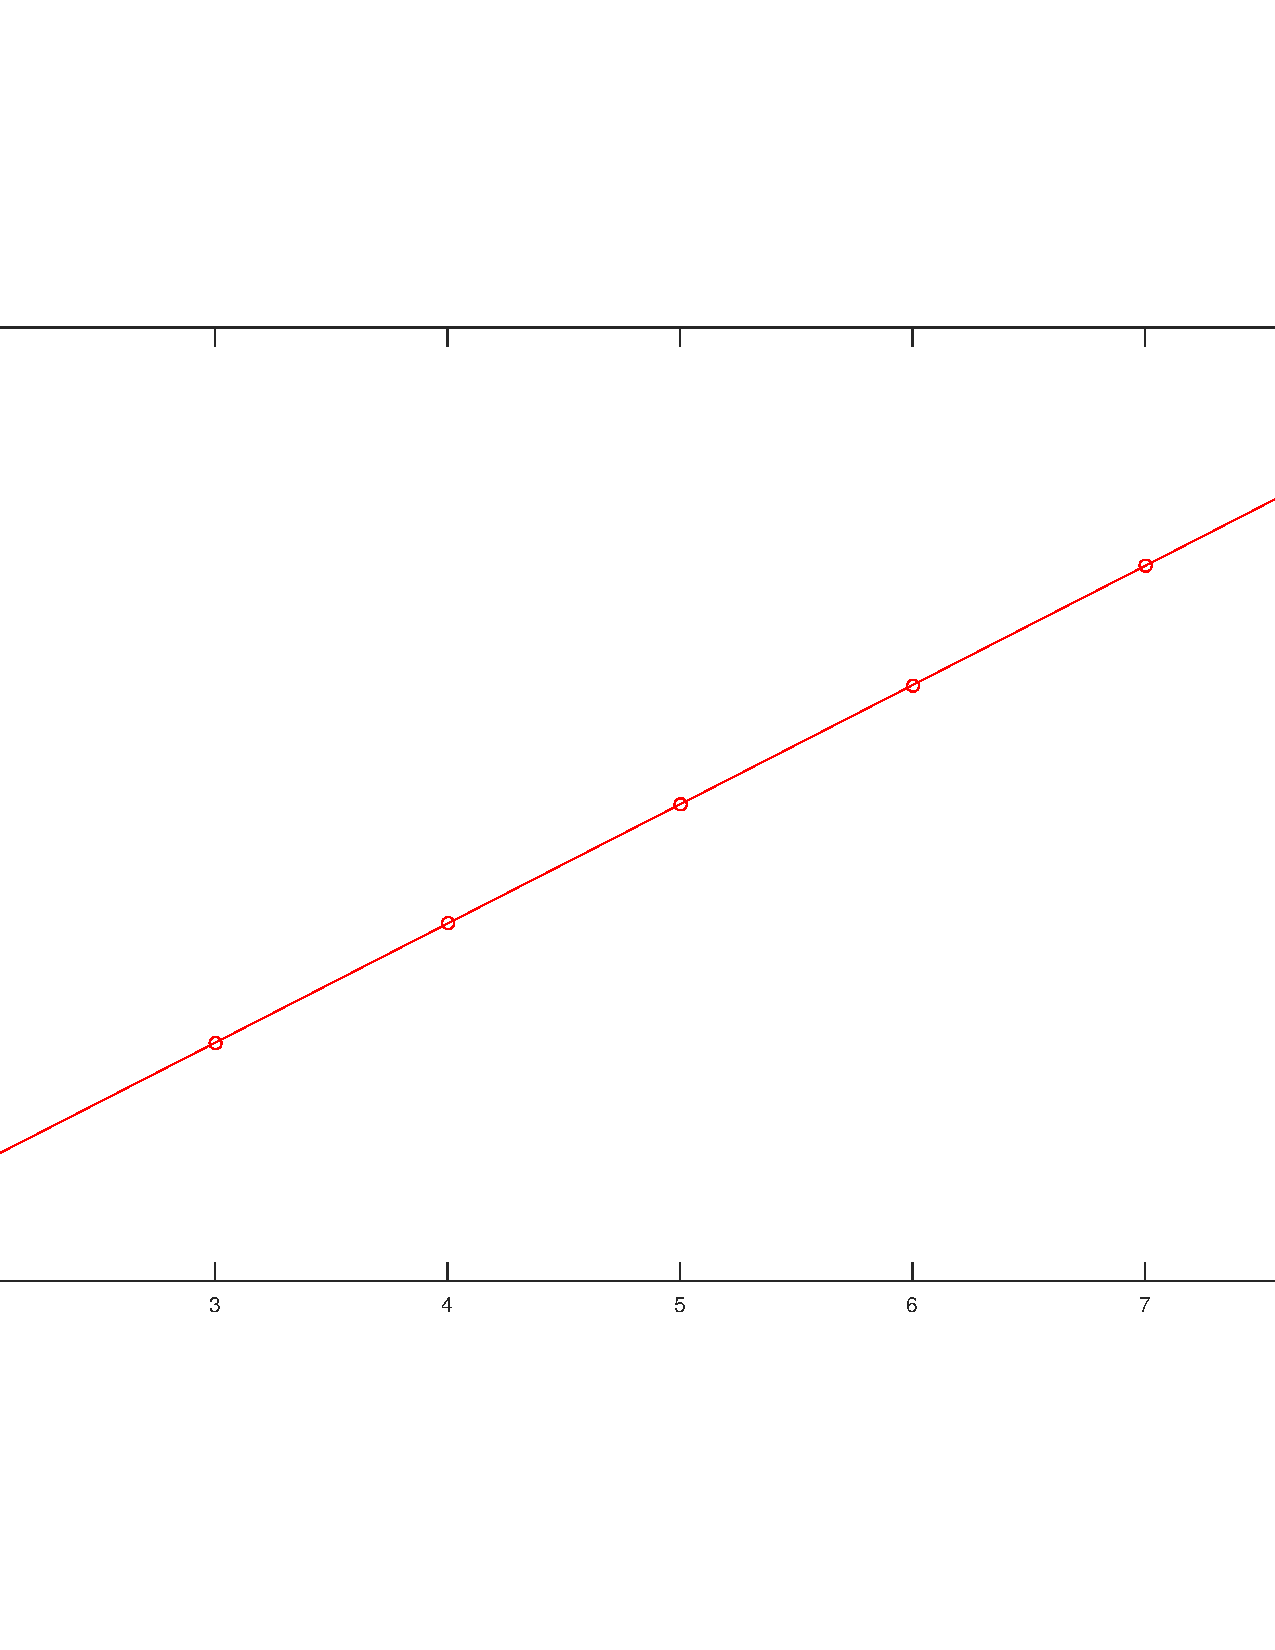
\includegraphics[width=\columnwidth]{replace_graph.pdf}}
% \caption{Plot of pneumatic cannon firing angle vs ending angle} 
% \label{fig:TradvsAutoDrop}
%\end{figure}






%%
%\section{Comparision}\label{sec:Comparision}


\begin{figure} \centering
  {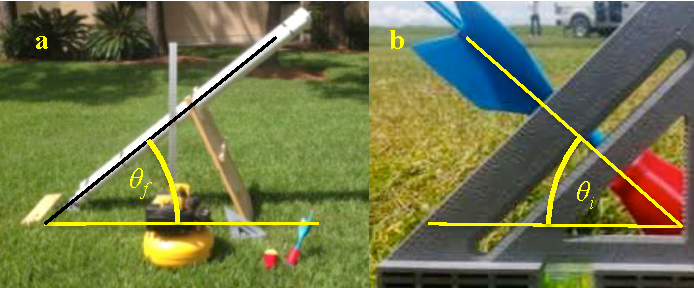
\includegraphics[width=\columnwidth]{CannonPicture}}
 \caption{A pneumatic launcher for SeismicDarts.  Ballistic dart deployment has limited usefulness because the incident angle is equal to the firing angle.} 
 \label{fig:CannonPicture}
\end{figure}

\begin{figure*}[htb]
\centering 
\vspace{1em}
\renewcommand{\figwid}{0.5\columnwidth}
\begin{overpic}[width =\figwid]{sim1_1.pdf}
\end{overpic}
\begin{overpic}[width =\figwid]{sim1_2.pdf}
\end{overpic}
\begin{overpic}[width =\figwid]{sim1_3.pdf}
\end{overpic}
\begin{overpic}[width =\figwid]{sim1_4.pdf}
\end{overpic}
\caption{Screenshots of simulations that were performed to estimate time take by different sensors surveying 100x100 m grid: a.) only SeismicSpiders b.) SeismicDarts and deployment system c.) heterogeneous system d.) human workers.
\label{fig:Sim_overview}}
\end{figure*}

\subsection{Ballistic Deployment}
To compare an alternative deployment mechanism we built the pneumatic cannon shown in Fig.~\ref{fig:CannonPicture}a.
The pneumatic cannon is U-shaped,  2 m in length, with a 0.1 m (4 inch) diameter pressure chamber and a 0.08 m (3 inch) diameter firing barrel, connected by an electronic valve (Rain Bird JTV/ASF 100). 
The cannon is aimed by selecting an appropriate firing angle $\theta_f$, azimuth angle, and chamber pressure.  
The reachable workspace is an annular ring whose radius $r$ is a function of the firing angle and initial velocity $v$. 
Neglecting air resistance, this range is found by integration:
\begin{align}
r = \frac{v^2}{g} \sin( 2 \theta_f )
\end{align} 
Initial velocity is limited by the maximum pressure and size of the pressure chamber.
The cannon used  SCH 40 PVC, which is limited to a maximum pressure of 3 Mpa (450 psi).

We charged our system to 1 Mpa (150 psi), and achieved a range of $\approx$ 150 m.
This range is considerably smaller than the UAV's range, which when loaded can complete a round trip of $\approx 1.5$ km.

A larger problem, illustrated in Fig.~\ref{fig:CannonPicture}, is that angle of incidence $\theta_i$ is equal to the firing angle $\theta_f$. 
Maximum range is achieved with $\theta_f = 45^\circ$, but this angle of incidence reduces the geophone sensitivity to $\cos(\theta_f )\approx 0.7$.
The placement accuracy of the cannon is lower than the UAV because a fired dart must fly over a longer distance than a dropped dart. 
Safety reasons also limit applications for a pneumatic launcher.





\begin{table} \centering
  {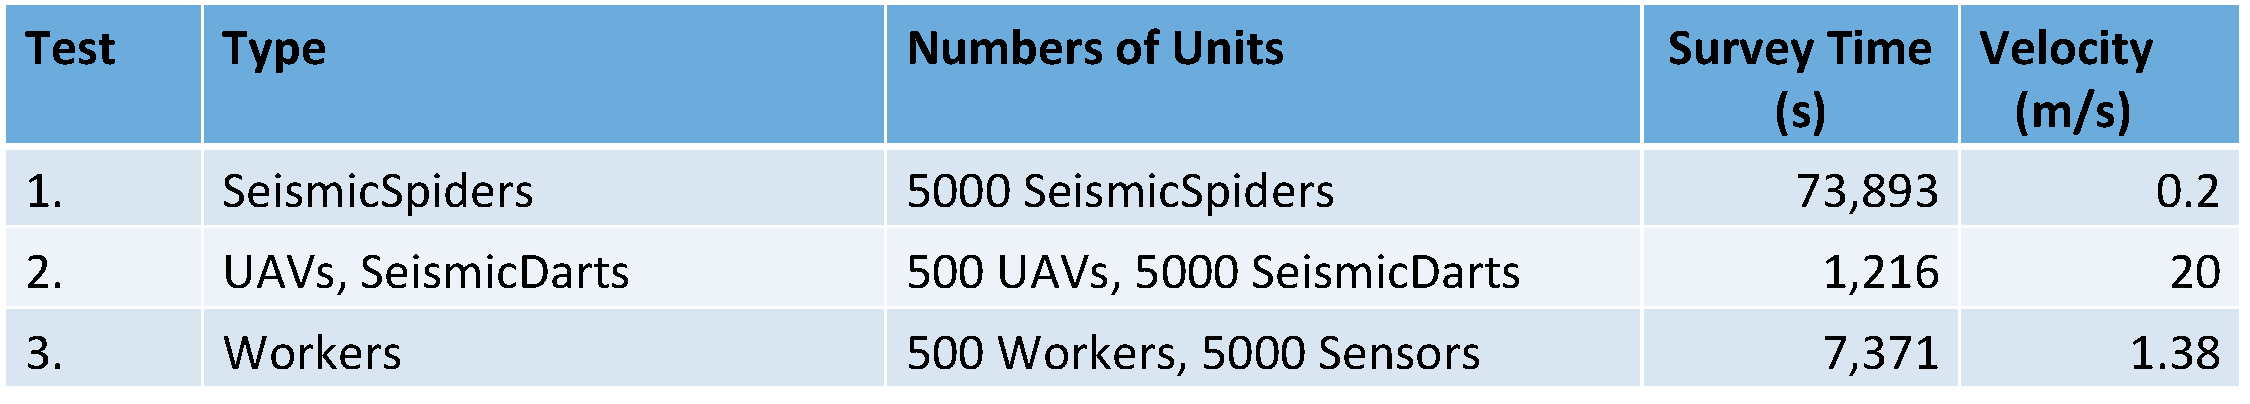
\includegraphics[width=\columnwidth]{simulation_table.pdf}}
 \caption{Comparison of different  deployment modes highlights the efficiency of UAV deployment.} 
 \label{tab:Sim_table}
\end{table}

\begin{figure} \centering
  {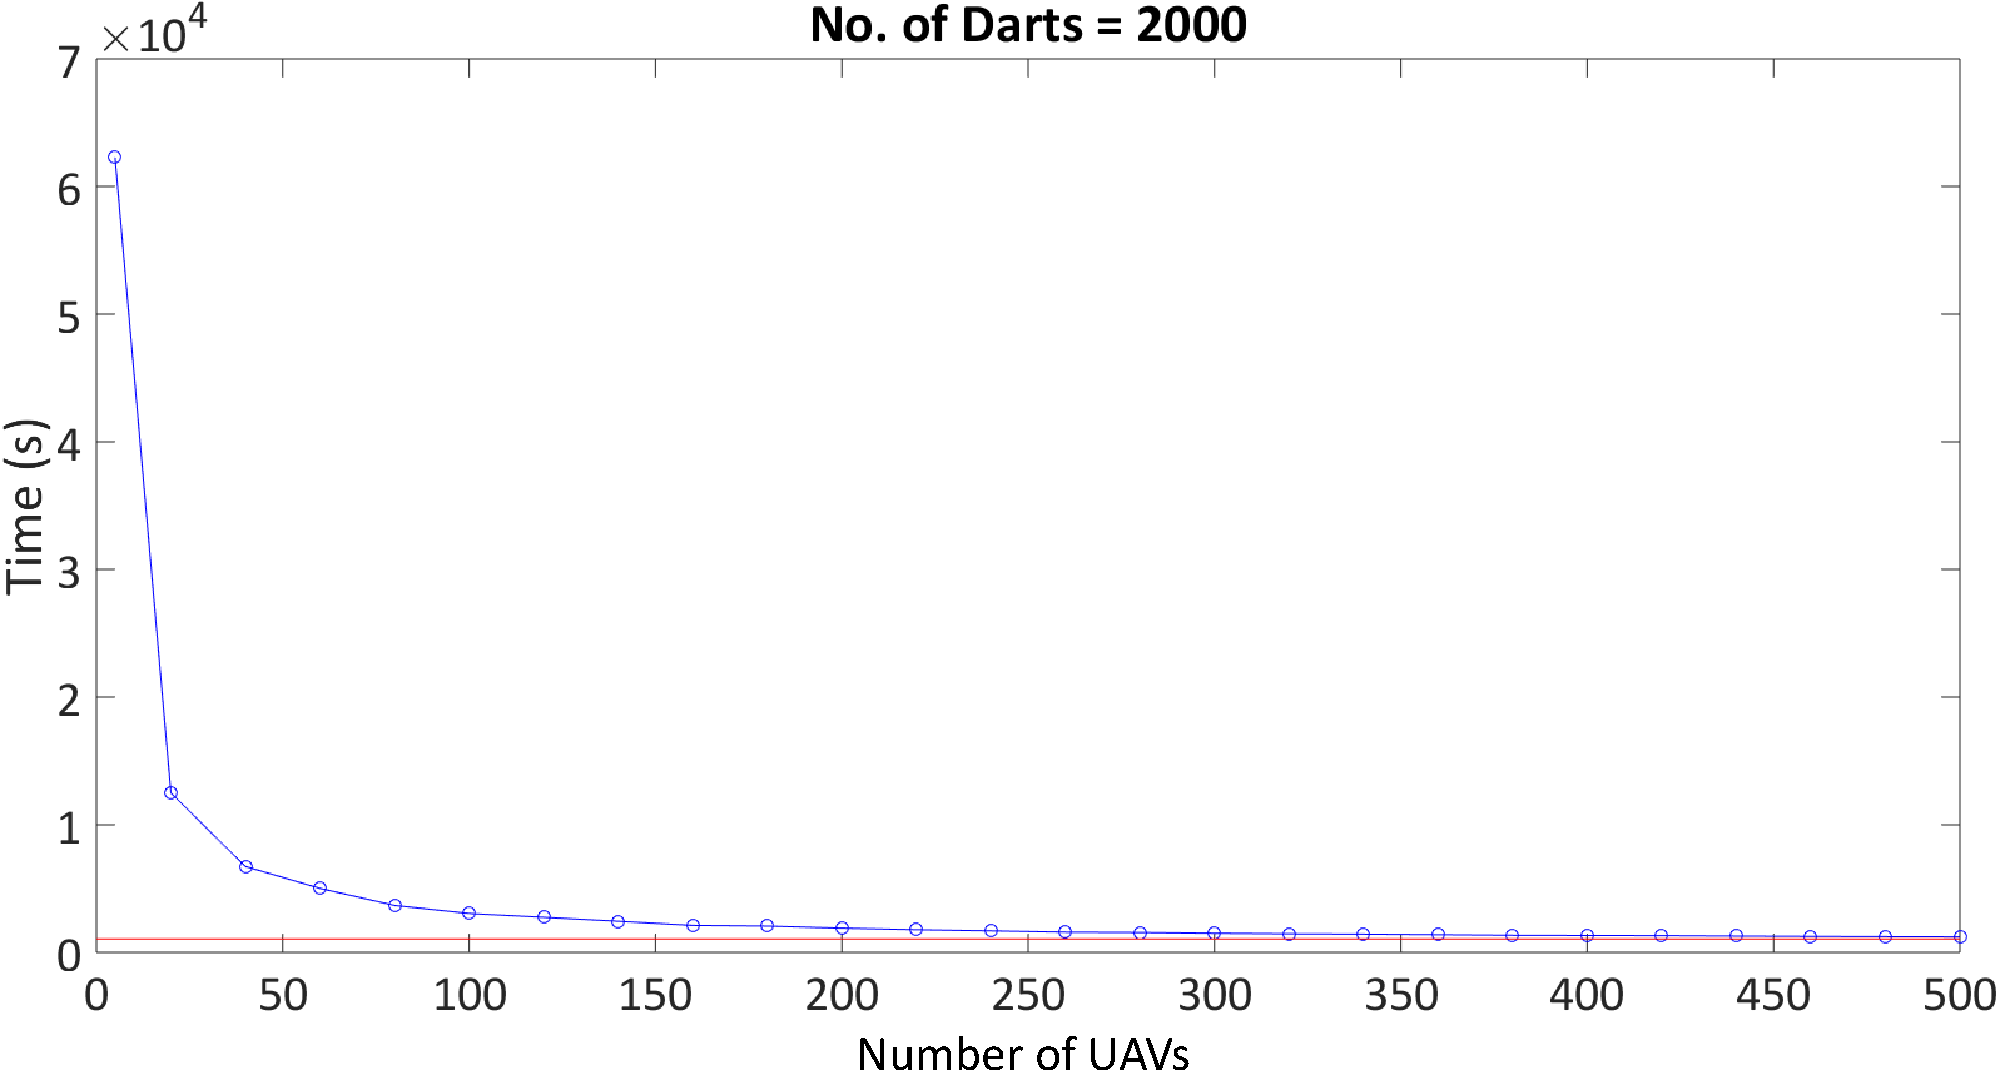
\includegraphics[width=\columnwidth]{DronevsTime.pdf}}
 \caption{Survey time for a 1km x 10 km region for different numbers of UAVs.} 
 \label{fig:DronevsTime}
 \vspace{-1em}
\end{figure}

\begin{figure} \centering
  {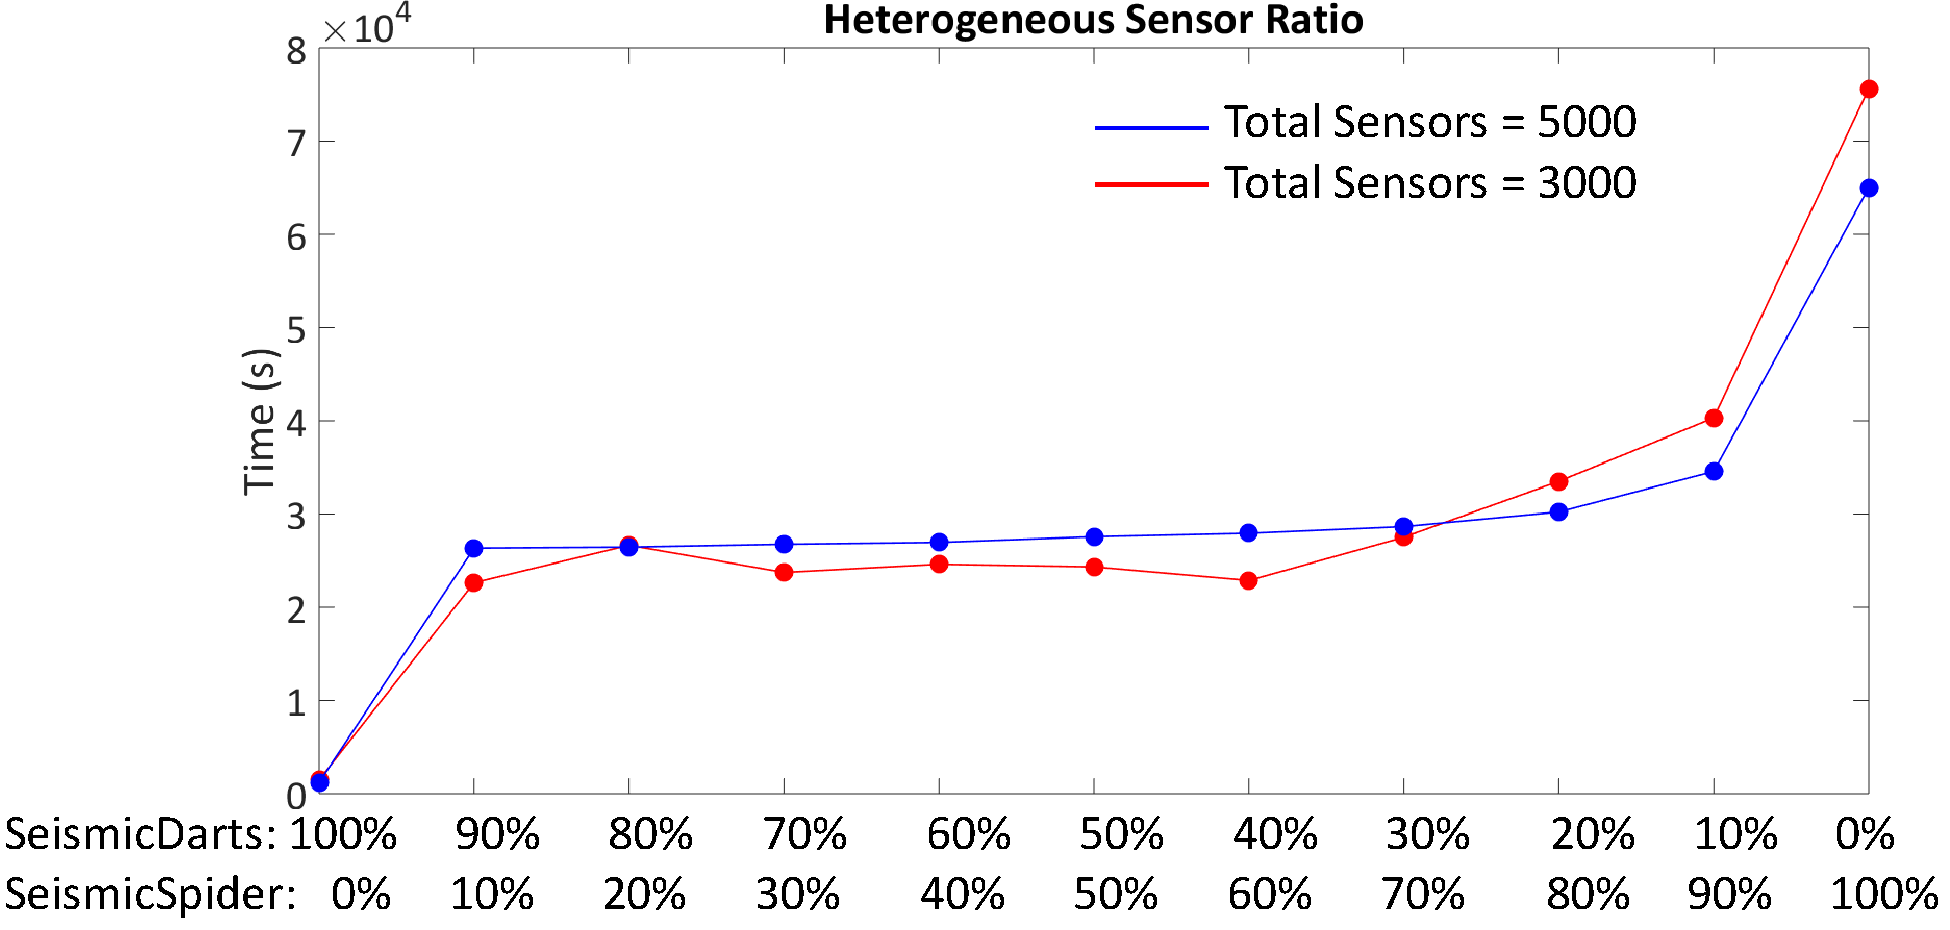
\includegraphics[width=\columnwidth]{het_sen_ratio.pdf}}
 \caption{Survey time for different sensor ratios. The total number of sensors \{5000, 3000\} were kept constant. Ten darts were provided for each UAV. } 
 \label{fig:het_sen_ratio}
  \vspace{-1em}
\end{figure}

\subsection{Simulation Studies}
   A scheduling system to compare  time and costs for seismic surveys with varying numbers of UAVs, SeismicSpiders, SeismicDarts, and human laborers was coded in  {\sc Matlab}, available at \cite{Srikanth2016seismicScheduler}.
% The goal of the Seismic Survey Scheduler is to estimate the requirements for a specific seismic survey. 
% The scheduler compare  time and costs for seismic surveys with varying numbers of UAVs, SeismicSpiders, SeismicDarts, and human laborers was coded in  {\sc Matlab}, available at \cite{Srikanth2016seismicScheduler}. 
   In each simulation, a seismic source must be measured at every survey point. 
   The scheduler must assign each sensor (SeismicDart or SeismicSpider) to an unmeasured survey point and assign each UAV or human worker a dart to pickup or deploy.  Once a sensor reaches a survey point, that sensor must wait until a seismic source is measured.
   A vibration truck (blue) provides the seismic source.
   Motion planning uses a centralized, greedy strategy.
   
   Frames from four different cases on a small survey region are shown in Fig.~\ref{fig:Sim_overview} on a 100x100 m area with survey points at 10 m spacing:
   a.) simulates 10 SeismicSpiders;  
   b.) simulates 5 SeismicUAVs deploying 50 SeismicDarts. Each UAV was allowed to carry up to 4 darts;
   c.) simulates 10 SeismicSpider, 5 SeismicUAVs and 50 SeismicDarts;
   d.) simulates 5 human workers deploying 75 SeismicDarts. Each worker was allowed to carry up to 10 darts. 
 Survey points are grey circles if unmeasured and green if measured.   The simulation uses red hexagons for SeismicSpiders,  black diamonds for UAVs,  inverted yellow triangles for SeismicDarts, and magenta diamonds for human workers. The assigned motion path for each sensor is colored magenta and the path completed is blue. 
 %The program simulates a seismic survey and records the time required. This allows comparing different combinations of sensing assets.

   
%  The first frame in Fig.~\ref{fig:Sim_overview} corresponds to SeismicSpiders (red hexagons) surveying a area of 100x100 m. 
%  Ten SeismicSpiders moving at a velocity of $0.1$m/s tries to visit each survey point (indicated by blue circles) on the map. 
%  Once ten of these sensors are at a new survey location the blue truck (Seismic source) perturbs the ground creating a seismic wave. The SeismicSpiders record the values at their current locations. 
%  Then they start moving to their next location and we repeat this process until we obtain readings at the survey locations. 
% % We follow a greedy approach to identify the SeismicSpiders new location.
%   The second frame in Fig.~\ref{fig:Sim_overview} corresponds to SeismicUAV (Black Diamond) deploying the SeismicDarts (inverted yellow triangle).
%    One SeismicUAV can carry four SeismicDarts simultaneously and drop them at different locations. 
%    Similar to the simulation involving the SeismicSpider once ten sensors are at a new survey point the blue truck takes a shot. 
%    The SeismicDarts record the readings at their corresponding locations.
%     Once this is done the SeismicUAV will pick up these SeismicDarts and redeploy them at new survey point.
%     % We follow a greedy approach to deploy these sensors. 
%      The third frame in Fig.~\ref{fig:Sim_overview} combines the SeismicSpider and SeismicDarts.
%       This represents a heterogeneous system surveying. 
%       The fourth frame in Fig.~\ref{fig:Sim_overview} represents human workers (magenta diamonds) servicing a region.
%        In all the simulations red lines connect the sensor location the sensor just surveyed to it's new location. 
%        The blue line connects the location the sensor just surveyed to it's current location. 
%        All sensors are assumed to start from the blue truck at $T = 0$. 
%        The Seismic Survey  simulates the proposed system and comparison with manual deployment could be achieved for analysis. 
%        The simulator is robust and all the parameters described above are variables. 
%        We want this tool to be used for preprocessing of a seismic survey in which you can vary the number of sensors, velocity, size of seismic survey, location of the seismic source etc.
%         Using this simulator we can closely match a real seismic survey and thus optimize the resources.
 

%A scheduling system to compare  time and costs for seismic surveys with varying numbers of UAVs, SeismicSpiders, SeismicDarts, and human laborers was coded in  {\sc Matlab}, available at \cite{Srikanth2016seismicScheduler}. Frames from four different cases are shown in Fig.~\ref{fig:Sim_overview}.

This tool allows us to examine engineering and logistic trade-offs quickly through simulations.  For example, Fig.~\ref{fig:DronevsTime} assumes a fixed number of darts and examines the finishing time with $5$ to $500$ UAVs.  The time required decays asymptotically, but $140$ UAVs requires only twice the amount of time required for $500$ UAVs, indicating  $140$ UAVs are sufficient for the task.    
 Substantial cost savings can be obtained by selecting the number of UAVs required to complete within a certain percentage greater than the optimal time.

The tool is useful for comparing the effectiveness of heterogeneous teams.  Table~\ref{tab:Sim_table} compares surveying a $1$ km x $10$ km strip of land with teams of (a) $5000$ SeismicSpiders, (b) $500$ UAVs and $5000$ SeismicDarts, (c) $500$ humans and $5000$ geophones.  Team (b) completed six times faster than team (c). 
  Since SeismicSpiders are  slower than UAVs and humans and are expensive compared to the SeismicDarts, their use is limited to special occasions. The UAV can deploy the SeismicSpider at a given waypoint. This attribute was not considered in the simulation but would improve deployment speed of SeismicSpiders.
   
In Fig.~\ref{fig:het_sen_ratio}, the total number of mobile agents are constant, but the percentage of UAVs and SeismicSpiders are varied.  10 SeismicDarts were provided for each UAV. Increasing the percentage of UAVs lowers the deployment time because UAVs move 20 m/s but SeismicSpiders move 0.2 m/s. 
The velocity difference makes UAV deployment time-efficient. 

%%
%% Thesis 

\chapter[Conclusion]{Conclusion}
\label{chap-conc}

In this thesis, three applications for autonomous unmanned vehicles were presented.
Unmanned aerial vehicles (UAV) can be used to deploy, retrieve geophones for seismic surveying and deploy unmanned rover attached with geophones.
We presented software to plan for a wireless sensor network deployment using UAV and unmanned rover.
A UAV was used to drag an electrified net through an area to destructively survey mosquito populations.
We used our collaborator's algorithm to reduce the energy expenditure while maximizing area covered.
An updated design for drifting wireless sensor node was presented.
The drift node can be used to survey coastlines and national maritime boundaries for marine border security, wildlife science missions.

In future work, the applications above could be merged together for a more complete package.
A wireless sensor network can then be deployed, monitored and retrieved by AUVs.
Before the WSN deployment, the area can be surveyed by a UAV with minimal energy expenditure.
Wireless sensor nodes can communicate with each other to relay position, cache data or relay data back to the base station.
Like in \cite{sudarshanwsn}, UAVs can monitor data and charge wireless sensor nodes, extending their longevity.
For destructive mosquito surveying methods, the UAVs can incorporate live data to plan its route reactively.

%We developed a method to deploy geophones for seismic surveying with AUVs, reducing manual labors and injury risks.
%The geophones are combined with a data recording unit, can record its own position and the soundwave during the seismic survey.
%This eliminate long analog data transmisison cables, which reduce a large part of equipment weight during surveying.
%We can drop geophones from our UAVs when we put the geophones a SeismicDart shell, which eliminates the need for a separate UAV per sensor.
%For terrains that UAVs cannot fly to or the SeismicDart cannot approach, we developed a SeismicSpider, with geophones for legs.
%The SeismicSpider can travel to its desired position, with geohphones contacting the ground, record the soundwave during the survey.
%The software we developed to schedule a seismic survey can be used for many other wireless sensor network applications that use UAVs and autonomous rovers.

%
%
%\bibliographystyle{IEEEtran}
%\bibliography{./bibs/match}
%
%% that's all folks
%\end{document}
%
%

%Using a UAV for Destructive Surveys of Mosquito Population
\chapter[UAV Surveying Mosquitoes]{Using a UAV for Destructive Surveys of Mosquito Population}

This chapter presents research performed for the ICRA paper "Using a UAV for Destructive Surveys of Mosquito Population", by A. Nguyen, D. Krupke, M. Burbage, S. Bhatnagar, S.P. Fekete, and A.T. Becker.

I constructed the UAV and the attachment of the net, as well as assisted in early generations of the net. I piloted all UAV test and programmed the autonomous tests of our algorithm and data collection. I also designed the method to measure powerconsumption of the UAV and analyzed the data.

\section[Overview And Related Work]{Overview And Related Work}
%%%%%%%%%%%%%%%%%%%%%%%%%%%  

\noindent  \emph{Mosquito Control Solutions}:
Mosquito control also has a long history of efforts associated both with monitoring mosquito populations~\cite{dennett2007associations} and with eliminating mosquitoes.
The work involves both draining potential breeding grounds and destroying living mosquitoes~\cite{peter2005tick}.
An array of insecticidal compounds has been used with different application methods, concentrations, and quantities, including both larvicides and compounds directed at adult mosquitoes~\cite{larvicides2005guidelines}.

Various traps have been designed to capture and/or kill mosquitoes with increasing sophistication in imitating human bait, as designers strive to achieve a trap that can rival the attraction of a live human~\cite{maliti2015development}.
In recent history, methods have also included genetically modifying mosquitoes so that they either cannot reproduce effectively or cannot transmit diseases successfully~\cite{marshall2009malaria}, and with the recent genomic mapping of mosquito species, new ideas for more targeted work have been formulated~\cite{hill2005arthropod}.

Popular methods to control mosquitoes such as insecticides are effective, but they have the potential to introduce long-term environmental damage and mosquitoes have demonstrated the ability to become resistant to pesticides~\cite{ndiath2012resistance}.
Traditional electrified screens (bug zappers) use UV light to attract pests but have a large bycatch of non-pest insects~\cite{University-Of-Florida1997}
This chapter introduces techniques using bug zappers mounted on unmanned vehicles to autonomously seek out and eliminate mosquitoes in their breeding grounds and swarms.
Instrumentation on the bug zappers logs the GPS location, altitude, weather details, and time of each mosquito hit.
Mosquito control offices can use this information to analyze the insects' activities.
The device can be mounted on a remote-controlled or autonomous unmanned vehicle.
If autonomous, the vehicle can use the data collected from the electrified screen as feedback to improve the effectiveness of the motion plan. 
	
\noindent  \emph{Robotic Pest Management}:
As GPS technology has flourished and data processing has become cheaper and more readily available, researchers have explored options for implementing the new technologies in breeding ground removal~\cite{anupa2014identification} and more effective insecticide dispersion~\cite{hur2015low}.  Low-cost UAVs for residential spraying are under development~\cite{amenyo2014medizdroids}.  Even optical solutions have been considered, including laser containment~\cite{boonsri2012laser} or, by extension, exclusion and laser tracking and extermination~\cite{kare2010build}.
    
\noindent \emph{Robotic Coverage}: 
Robotic coverage has a long history. The basic problem is one of designing a path for a robot that ensures the robot visits within $r$ distance of every point on the workspace.  For an overview see~\cite{Choset2001}.  This work has been extended to use multiple coverage robots in a variety of ways, including using simple behaviors for the robots~\cite{spears2006physics,Koenig2001}.

The classic \emph{Travelling Salesman Problem (TSP)} is generalized to the \emph{Lawnmower Problem} \cite{arkin2000approximation}, which try to cover the most area with a tool of a nontrivial size.
For minimizing the turn cost of coverage path, Arkin et al.~\cite{arkin2005optimal} showed that finding minimum turn tours in grid graphs is NP-hard.
The complexity of finding a set of multiple cycles that cover a given set of locations at minimum total turn cost had remained elusive for many years; \emph{Problem~{53}} in \emph{The Open Problems Project}~\cite{openproblemproject} asks for the complexity of finding a minimum-cost (full) cycle cover in a 2-dimensional grid graph.
Arkin et al. showed~\cite{arkin2005optimal,arkin2001optimal} that the full coverage variant in {\em thin} grid graphs (which do not contain a $2\times 2$ square,
so every pixel is a boundary pixel) is solvable in polynomial time. Fekete et al.~\cite{dom3} were able to resolve this issue by showing that finding a cycle cover of minimum turn cost is  NP-hard.

\section[Hardware Design]{Hardware Design}
%%%%%%%%%%%%%%%%%%%%%%%%%%%%%%%%%%%%%%%

This section examines the components of the mosquito UAV system, shown in Fig.~\ref{fig:DroneAndNet}. This includes the UAV, electrified screen, surveying electronics, and a discussion of the energy budget. 
%The design for the mosquito UAV system been assigned a U.S.\ Provisional Patent Application~\cite{Becker2016patentapp}.

\subsection{The UAV}

The UAV is a custom-built, $\SI{177}{\centi\metre}$ wingspan hexacopter, controlled by a Pixhawk flight controller running ArduPilot Mega flight software. The UAV has a 3DR GPS module using the UBlox NEO-7 chipset.

\subsection{Screen Design}
The mosquito screen is designed to eliminate high density mosquito populations. 
This screen was constructed from two expanded aluminum mesh panels, spaced apart by \SI{3}{\milli\metre} thick ABS grid. 
These mesh panels have \SI{12}{\milli\metre} diamond-shaped  openings, and is held taught by nylon bolts around the perimeter.  
The bottom mesh panel is offset by half a diamond (6 mm) to the right to ensure all insects greater than 6 mm cannot pass through the net.
The top mesh is held at the reference voltage and the bottom mesh is energized to $1.8~kV$ above the reference voltage.

The perimeter is reinforced by two sets of \SI{7}{\milli\metre} diameter fiberglass rods that are inset into 3D printed corner fixtures.
These rods protect the frame from getting damaged from any side, and allows the UAV to land without damaging the net.


Once assembled, the net weighs \SI{0.948}{\kilogram} and has an overall area of \SI{0.194}{\square\metre}, with the spacer occupying \SI{0.0325}{\square\metre}. 
This makes the effective net area \SI{0.161}{\square\metre}. %, and the total cost of building a net this size is only \$27.44 USD.



%Design files and build instructions are available at~\cite{Vinh2016BugNet}.


%%%%%%%%%%%%%%%%%%%%%%%
\subsection{Screen Location}
The UAV carries the bug-zapping screen, which is suspended by paracord rope at each corner.  The location of this screen determines the efficacy of the mosquito UAV, measured in mosquitoes detected per second of flight time. The following describes a simplified analysis to optimize the screen location.

For manufacturing ease, the electrified screen is a rectangle with a width of $d_s$. The screen is suspended a distance $h_s$ beneath the UAV flying at height $h_d$.  We chose to suspend the screen beneath the UAV to avoid the weight of the rigid frame that would be required if the screen were above the UAV and because most mosquito species prefer low flight~\cite{gillies1976vertical}.  This screen can be suspended at any desired angle $\theta$ in comparison to horizontal, as shown in Fig.~\ref{fig:DroneConfigs}.
Two key parameters are the distance $h_s$ and the optimal angle $\theta$.  The goal is to clear the greatest volume of mosquitoes per second, a volume defined by the UAV forward velocity $v_f$ and the cross-sectional area $h_m \times d_s$ cleared by the screen, as shown in Fig.~\ref{fig:AngleVsSpeed}.

To hover, the UAV must push sufficient air down with velocity $v_d$ to apply a force that cancels the pull of gravity.  The UAV and screen combined have mass $m_{d}$ and its cross section can be approximated as a square with a side length of $d_d$.  The mass flow of air through the UAV's propellers is equal to the product of the change in velocity of the air, the density of the air $\rho_a$, and the cross sectional area.

\begin{figure}
\centering
\begin{overpic}[width=\columnwidth]{icra2018/DroneConfigs.pdf}\end{overpic}
\caption{\label{fig:DroneConfigs}
The UAV suspends a rectangular bug-zapping screen beneath it.  Propwash pushes incoming mosquitoes downwards, and the UAV clears a volume $h_m \times d_s \times v_f$ each second. Circles show two mosquitoes at equal time intervals relative to the UAV.} 
\vspace{-1em}
\end{figure}


We assume that air above the UAV is quiescent, so the change in velocity of the air is $v_d~ \si{\metre\per\second}$.
\begin{align} \label{eq:forceBalanceForDrone}
\text{Force gravity} & = \left(\text{mass flow}\right) \cdot \text{air velocity} \nonumber \\
m_{d} \cdot  g &= (v_d \cdot  \rho_a \cdot  d_d^2 ) \cdot  v_d 
% \text{kg} \cdot \frac{ \text{m}}{ \text{s}^2}&= \left( \frac{ \text{m}}{\text{s}} \cdot  \frac{ \text{kg}}{\text{m}^3}  \cdot \text{m}^2 \right) \cdot  \frac{ \text{m}}{\text{s}}\nonumber
\end{align}

Then the required \emph{propwash}, the velocity of air beneath the UAV, for hovering is
\begin{align} \label{eq:dronePropwash}
v_d = \sqrt{ \frac{ m_d g}{\rho_a d_d^2} }
\end{align}
The flight testing site in Houston, Texas is \SI{15}{\metre} above sea level. At sea level the density of air $\rho_a$ is \SI{1.225}{\kilogram\per\cubic\metre}.
The UAV and instrumentation combined weigh \SI{5.1}{\kilogram} with a width of \SI{0.75}{\metre}. The acceleration due to gravity is \SI{9.871}{\metre\per\square\second}.  Substituting these values gives $v_d = \SI{8.5}{\metre\per\second}$.

Due to propwash, an initially hovering mosquito will fall when under the UAV at a rate of $v_d$.  Relative to the UAV, the mosquito moves horizontally at a rate of $-v_f$.  As shown in Fig.~\ref{fig:DroneConfigs}, we can extend lines with slope $-v_d/v_f$ from the screen's trailing edge to $h_{\textrm{top}}$ and from the leading edge to $h_{\textrm{bottom}}$.
\begin{align} \label{eq:ClearedCrossSection}
h_{\textrm{top}} &= h_d - h_s + \frac{d_s}{2} \sin(\theta) +  \frac{d_d + d_s\cos(\theta)}{2}  \frac{v_d}{v_f} \nonumber \\
h_{\textrm{bottom}} &= h_d - h_s - \frac{d_s}{2} \sin(\theta) +  \frac{d_d - d_s\cos(\theta)}{2}  \frac{v_d}{v_f}  \nonumber \\
h_m &= h_{\textrm{top}} - h_{\textrm{bottom}} =  d_s\left(\frac{v_d}{v_f}\cos(\theta) + \sin(\theta) \right)
\end{align}
The optimal angle is therefore a function of forward and propwash velocity:
\begin{align} \label{eq:OptimalScreenAngle}
\ \theta = \mathrm{ArcTan}\left(\frac{v_f}{v_d}\right)
\end{align}

To ensure the maximum number of mosquitoes are collected, the screen must be sufficiently far below the UAV $ h_s > \frac{d_s}{2} \sin(\theta) +  \frac{d_d + d_s\cos(\theta)}{2}  \frac{v_d}{v_f}$  and the bottom of the screen must not touch the ground, $ h_d > h_s + \frac{d_s}{2} \sin(\theta) $.

\begin{figure}
\centering
\begin{overpic}[width=\columnwidth]{icra2018/AngleVsSpeed.pdf}\end{overpic}
\caption{\label{fig:AngleVsSpeed}
The volume cleared by a UAV is a function of screen angle $\theta$ and forward velocity $v_f$.  Dotted line shows the optimal angle given in \eqref{eq:OptimalScreenAngle}. } 
\vspace{-1em}
\end{figure}

There are practical limits to $h_s$ as well.  Tests with $h_s > \SI{2}{\metre}$ were abandoned because the long length caused the screen to act as a pendulum, introducing dynamics that made the system difficult to fly.

Changing the flying height $h_d$ of the UAV will target different mosquito populations because mosquitoes are not distributed uniformly vertically. 
Gillies and Wilkes demonstrated that different species of mosquitoes prefer to fly at different heights~\cite{gillies1976vertical}. 

%%%%%%%%%%%%%%%%%%%%%%%
\subsection{Wind Tunnel Verification of Net Angle}

This section describes experiments run in a wind tunnel to verify the simplified net angle analysis in the previous section. 
Smoke streaklines were used to visualize the flow of air as it passed by the UAV.
Due to space constraints in the wind tunnel, a free-flying phantom 4 was used instead of the hexacopter used for carrying the zapper. 
The wind tunnel was set to a \SI{3}{\metre\per\second} flow speed, and the UAV manually flown in approximately stable hovering.
The solo UAV is \num{0.3} $\times$ \num{0.3} $\times$ \SI{0.2}{\metre}.  The windtunnel has a \SI{1}{\metre} $\times$ \SI{1}{\metre} cross section. 
%??? brand name of the smoking apparatus?
As seen from Fig.~\ref{fig:WindTunnel}, the proposed screen position captures free flowing air and air entrained by the UAV propellers.
This test encouraged us to mount the net as close to the UAV as possible, so that air, and flying mosquitos, entrained by the propellers are pushed into the net.


\begin{figure}
\centering
\begin{overpic}[width=1.0\columnwidth]{icra2018/WindTunnelv01lowres.pdf}\end{overpic}
\caption{\label{fig:WindTunnel}
	Frames from wind tunnel test with free-flying UAV at \SI{3}{\metre\per\second} windspeed with smoke for streaklines~\cite{Bhatnagar2018}.  As shown in the frames at right, the proposed screen position (in red) captures free flowing air and air entrained by the UAV propellers.
	Each black square is \SI{25.4}{\milli\metre} in width.
} \vspace{-1em}
\end{figure}


%%%%%%%%%%%%%%%%%%%%%%%
\subsection{Data Logger}

The electrical detection and logging system is powered by a $9~V$ lithium ion battery applied directly to the controller and two AA $3~V$ lithium ion batteries applied to the power circuit for the screen.
The controller uses a GPS shield for monitoring the location and altitude as well as a real time clock to timestamp each data point collected from the system.
A Raspberry Pi 3 is used for data logging, 
sensors include a GPS sensor (NEO-6M Ublox), 
a capacitive humidity sensor, a thermistor (DHT22),
%ADS1115 16-bit ADC for monitoring the supply-side voltage of the net, and 
and an INA219 high side, 12-bit DC current sensor for monitoring the supply-side current delivered to the net.
The net current draw is logged at 100 Hz, while GPS and weather sensor data is logged at 1Hz.  
All data is stored on an onboard SD card.

%%%%%%%%%%%%%%%%%%%%%%%
\subsection{Energy Budget}

\begin{figure}
\centering
\begin{overpic}[width=0.9\columnwidth]{icra2018/OscilloscopeTrace.pdf}\end{overpic}
\caption{\label{fig:BugZapTrace}
					  Current, voltage, and power traces for five \textit{Culex quinquefasciatus} mosquitoes as each contacts the bug-zapping screen at $t=0$.  Contact causes a brief short that recovers in $\SI{160}{\milli\second}$.
} 
\vspace{-1em}
\end{figure}
% \todo{what is the new energy usage of the screen?}


Tests with an oscilloscope show that in the steady state, a $\SI{30.5}{\centi\metre} \times \SI{61}{\centi\metre}$ screen and electronics have a power consumption of \SI{3.6}{\watt}.  During a zap, the screen voltage monitoring circuit shorts briefly when the mosquito contacts the screen.  Figure~\ref{fig:BugZapTrace} shows the time sequences for battery and screen voltages, current, and power during five mosquito zaps.  
% % WE COULD NOT JUSTIFY THIS EQUATION 
%%  The initial current spike recovery can be modeled with an exponential fit.
%%
% \begin{align} \label{eq:BugZapFit}
%i=69.1e^{-2.7\times10^4 t} ~A
%\end{align}
%%
%The fit in \eqref{eq:BugZapFit} gives a time constant of $36~\mu s$ for the short and a recovery time of $80~\mu s$. 
Multiplying voltage by current to find the instantaneous power ($p=iv$) and integrating the area under the power curve show a total energy consumption of \SI{4.2}{\milli\joule} for each zap.  Recharging the screen requires more power and is represented in the latter part of the curves.  The overall recovery time is about $\SI{160}{\milli\second}$.  Most of the energy is consumed charging and maintaining the charge on the screen rather than in zapping the mosquitoes.





%Data
%The files used for this run of simulations are as follows:
%MosquitoFlightSimv2p0.m
%MosquitoSimv2p2randombounce.m
%MosquitoSimv2p2boustrophedon.m
%MosquitoSimComparev1p0.m
%
%All are located in the Dropbox code folder.
%Raw data are located in the Excel file Simulation Results.xlsx.
%    

%%%%%%%%%%%%%%%%%%%%%%%%%%%%%%%%%%%%%% 
\section[Path Planning]{Planning minimal turn cost paths}
%%%%%%%%%%%%%%%%%%%%%%%%%%%%%  

\newcommand{\revised}[1]{{\color{red}#1}}

%The following section present an overview of the algorithm used in the paper's research, which was done by our collaborators in Germany:
%D. Krupke and S.P. Fekete of TU Braunsweig.

\subsection{Modelling Mosquito Density}
\label{subsec:modelling}
Due to a-priori knowledge of mosquitos' preferred habitats from entomology, we can model the density of mosqitos in a field we want to cover.
This knowledge will help us plan the most efficient path, killing the most mosquitos with the least amount of energy used.
First, we divide a field for coverage into a pixel grid, the size of each pixel dictated by the size of the net and the resoultion of the UAV's GPS.
Each pixel $p_i\in P$ we give a relative density value $c(p_i)$ that describes the estimated mosquito density based on the environmental factor of the pixel.
In $P$ there will only be a subet with high relative density value.
The goal is to maximize the density covered by the set $S\subseteq P$ of visited pixels i.e., $\max_{S\subseteq P} \sum_{p_i\in S} c(p_i)$ within the available battery capacity.
This could be done in one single trip or over multiple trips with multiple batteries.

%The data on the distribution of mosquitoes is given for a two-dimensional grid environment; the grid size
%is induced by the size of the screen, the available data and the desired resolution of the extracted map. 
%For each pixel $p_i\in P$, we are given a relative value
%$c(p_i)$ that describes the estimated a-priori density of mosquitoes, based on data obtained from boustrophedon (back and forth) scans of the area by the UAV;
%this implies that only a subset of pixels carry a significant value.
%Visiting one of the pixels corresponds to sampling and mapping the actual density distribution of mosquitoes. 
%For a dense distribution of mosquitoes
%(which is the case for the instances relevant for pest control), multiple visits to the same pixel do not contribute additional
%knowledge. As a consequence, the objective is to maximize the sampling value of the set $S\subseteq P$ of visited pixels, 
%i.e., $\max_{S\subseteq P} \sum_{p_i\in S} c(p_i)$ {within the available battery capacity}; this may be over the course of a single closed trajectory, or over
%a combination of multiple roundtrips. 

\subsection{Turn Cost}

\begin{figure}[h]
\begin{center}
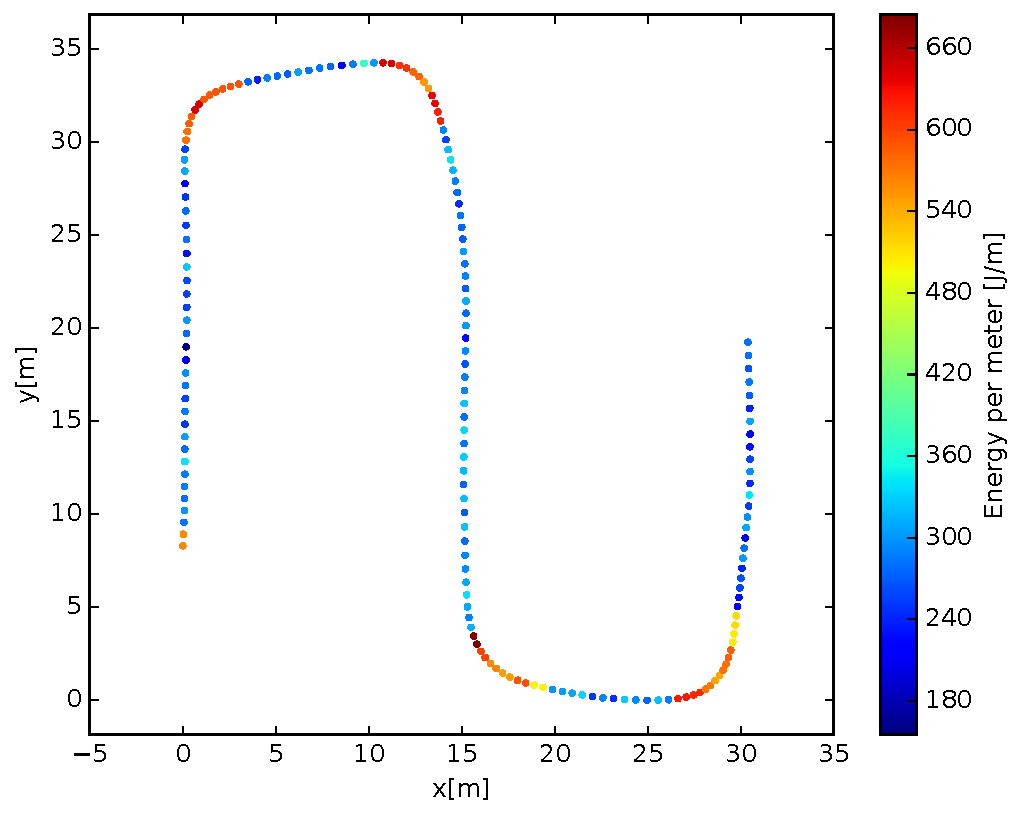
\includegraphics[width=.75\columnwidth]{icra2018/turncost}
\caption[Mosquito hunting drone]{Turns are expensive. See our related video at
\url{https://youtu.be/SFyOMDgdNao} for details, and
\cite{becker2017zapping} for an accompanying abstract.} \label{fig:turncost}
\end{center}
\vspace{-1em}
\end{figure}

UAVs can make turns on the spot, without curvature constraints like a fix-winged aircraft.
However, UAVs turns are energtically expensive.
As Fig.~\ref{fig:turncost} shows, the energy required per meter of travel in a turn is 4 to 5 times as expensive as traveling through a straight path.
The limiting factor for a UAV's flight is its battery capacity, therefor it is important to limit the amount of turns needed per flight while maximizing the amount of pixels visited.
To consider the total energy cost of a turn, we need to limit the types of turns the UAV made.
We consider only strict set of \ang{90} and \ang{180} turns since the UAV does not have minimal turn curvature.
Additionally, the two turn angles allow us to fly around most large obstacles while visiting the pixels around it.

%Planning good trajectories for a UAV is not subject to the same curvature constraints of an ordinary aircraft
%because UAVs can turn on the spot. However, turns are a critical aspect of path
%planning due to their impact on energy consumption.  Battery capacity is {\em the} limiting factor for  UAV flight time. As shown in Fig.~\ref{fig:turncost}, 
%the power output for a desired trajectory is non-uniform.  Flying along a straight path
%is relatively inexpensive but turning is energy intensive. 

%As a consequence, we must consider the total turn costs associated
%with changing direction, as measured by the turn angle.
%As we are not limited by trajectory curvature, we refer to straight-line connections and a finite set of $2\omega$ different
%headings for visiting vertices. For the most natural case of orthogonal grids $\omega=2$. When
%surveying non-isolated mosquito hotspots (whose size greatly exceeds the size of the UAV), we are not dealing with
%isolated pixels and the modeling error of this restriction is small.

%TODO: I guess one can save space here by e.g. skipping subset cover.
%Now we consider different trajectory types.
%A {\em cycle} is a roundtrip of a subset $S\subseteq P$ that visits all points in $S$ and returns to the origin, a {\em cycle cover} of $P$ is a set of cycles
%that together visit all points in $P$, and a {\em tour} is a single cycle that visits all points in $P$. A {\em subset cycle cover} for $S\subset P$ is a cycle
%cover that covers at least the points in $S$, while a {\em subset tour} is a tour of at least the points in $S$. For any of these structures, we are interested in
%%cycle covers or tours of {\em minimum total turn cost}. 
%{cycle covers or tours of {\em minimum total travel cost}. 
%The travel/battery cost is a linear combination of the number of pixel transitions (distance) and the weighted number of turns, 
%corresponding to the total turn angle.
%}
%In addition, a {\em minimum turn-cost penalty cycle cover}  or a {\em minimum turn-cost penalty tour}
%visits a subset $R\subset P$, such that the sum of total travel cost and the sum $\sum_{i\not\in R} c(p_i)$ of values of 
%unvisited pixels is minimized. 
%The travel/battery cost is a linear combination of the number of pixel transitions (distance) and the weighted number of turns, 
%corresponding to the total turn angle.
%Note that the travel cost
%may be a linear combination of turn and travel cost, as long as triangle inequality is satisfied.

%\subsection{Computational Complexity}
%\label{subsec:complexity}
%Finding optimal covering paths that map a given region is closely related to the famous 
%\emph{Traveling Salesman Problem (TSP)}, which asks to minimize
%total length of a single tour that covers all of a given set of locations. The TSP is one of 
%the classic NP-hard problems, so we cannot expect a general method that finds
%a provably optimal solution for any  instance in polynomially bounded time.
%A generalization of the TSP is
%the \emph{Lawnmower Problem} (see Arkin et al.~\cite{arkin2000approximation}, which considers coverage by
%a tool of nontrivial size. For the objective of minimizing the total cost (in particular, the turn
%cost), Arkin et al.~\cite{arkin2005optimal} showed that finding minimum-turn tours in grid graphs is NP-hard,
%even if a minimum-turn cycle cover is given. The complexity of finding a set of multiple cycles that cover a 
%given set of locations at minimum total turn cost had remained elusive for many years; \emph{Problem~{53}} in \emph{The Open Problems Project}
%%edited by Demaine, Mitchell, and O'Rourke~\cite{openproblemproject}
%asks for the complexity of finding a minimum-cost (full) cycle cover in a 2-dimensional grid graph. This is not 
%obvious: large parts of a solution can usually easily be deduced by local information and 2-factor techniques.
%Arkin et al. showed~\cite{arkin2005optimal,arkin2001optimal} that the full coverage variant in {\em thin} grid graphs (which do not contain a $2\times 2$ square,
%so every pixel is a boundary pixel) is solvable in polynomial time. In separate work~\cite{dom3}, two of us were able to resolve this
%issue by showing that finding a cycle cover of minimum turn cost is  NP-hard.

%\subsection{Mathematical Optimization}
%\label{subsec:complexity}
%A powerful approach for finding optimal solutions to instances of NP-hard problems is the use
%of Integer Programming (IP). While solving an IP still requires exponential time in the worst case,
%using carefully crafted mathematical models in combination with specific algorithm engineering and available
%IP solvers enables solving instances of considerable size to provable optimality.
%For our purposes, we can describe the problem as follows. 
%
%\paragraph{Penalty Cycle Covers}
%The set $P$ of pixels corresponds to a given grid graph $G(P,E)$ in which each pixel $p_j\in P$ is adjacent to the set $N(p_j)$
%of pixels in $P$ that share an edge with $p_j$.
%Each vertex $p_j\in P$ has a scalar reward $c(p_j)$ for visiting (or penalty for not visiting), 
%and a function $\text{cost}_j(i,k)\in \mathbb{Z}^+_0$  that maps the cost of traveling from $p_i$ to $p_j$ to $p_k$, where  $p_i,p_k\in N(p_j)$ are adjacent pixels to   $p_j$.
%This cost is symmetric, i.e. $\text{cost}_j(i,k)=\text{cost}_j(k,i)$. %TODO: Or cost(ijk) or cost(i,j,k) or cost(p_i, p_j, p_k)
%The integer program uses two types of variables: integer variables
%$x_{ijk}=x_{kji}$ that state how often passage $p_i-p_j-p_k$ or $p_k-p_j-p_i$ is used and
%Boolean variables $y_{j}$ that indicate that the pixel $p_j\in V$ is not covered,
%i.e., the penalty is paid.  This results in the following formulation: 
%%IP Formulation TODO
%%\begin{strip}
%%\begin{eqnarray}
%%	\min & \displaystyle  \sum_{p_j\in P} \sum_{p_i,p_k\in N(p_j)} \text{cost}_j(i,k) \cdot x_{ijk} + \sum_{p_j\in P}c(p_j) \cdot y_j\label{eq:obj}\\
%%	\text{s.t.}			& 1\leq\displaystyle 4 \cdot y_j +\sum_{p_i,p_k\in N(p_j)} x_{ijk} \leq 4&\forall p_j\in P \label{eq:ip:constr1}\\
%%						& \displaystyle 2 \cdot x_{jij} +\sum_{p_k\in N(p_i), p_k\not= p_j}x_{jik} = 2 \cdot x_{iji}+\sum_{p_k\in N(p_j), p_k\not= p_i}x_{ijk}  & \forall \{p_i,p_j\}\in E \label{eq:ip:constr2}\\
%%						& x_{ijk}\in\mathbb{N}_0, y_j\in \mathbb{B} & \forall p_j\in P, \{p_i,p_k\}\subseteq N(p_j)
%%\end{eqnarray}
%%\end{strip}
%\begin{eqnarray}
%	\min  \displaystyle  \sum_{p_j\in P} \sum_{p_i,p_k\in N(p_j)} \text{cost}_j(i,k) \cdot x_{ijk} + \sum_{p_j\in P}c(p_j) \cdot y_j\label{eq:obj}
%\end{eqnarray}
%with constraints
%\begin{eqnarray}
%	 1\leq\displaystyle 4 \cdot y_j +\sum_{p_i,p_k\in N(p_j)} x_{ijk} \leq 4, &\forall p_j\in P \label{eq:ip:constr1}
%\end{eqnarray}
%\begin{eqnarray}	
%%	\displaystyle  x_{jij}   \underset{ p_k\in N(p_i), p_k\not = p_j}{+ \tfrac{1}{2}\sum x_{jik}}  \!\!    =   x_{iji}      \underset{p_k\in N(p_j), p_k\not= p_i}{+ \tfrac{1}{2}\sum x_{ijk}},  & \forall \{p_i,p_j\}\in E 
%	\displaystyle 2 x_{jij}  \!\!\!   \underset{ p_k\in N(p_i), p_k\not = p_j}{+\sum x_{jik}}  \!\!\!\!\!    = 2  x_{iji} \!\!\!     \underset{p_k\in N(p_j), p_k\not= p_i}{+\sum x_{ijk}},  & \forall \{p_i,p_j\}\in E \label{eq:ip:constr2}
%\end{eqnarray}
%\begin{eqnarray}	
%	 x_{ijk}\in\mathbb{N}_0, y_j\in \mathbb{B} ,& \forall p_j\in P, \{p_i,p_k\}\subseteq N(p_j)  \label{eq:ip:constrINTS}
%\end{eqnarray}
%
%
%%Describe IP
%The objective function in Eq.~\ref{eq:obj} minimizes the total cost of the cycles and the uncovered pixels.
%Eq.~\ref{eq:ip:constr1} enforces a pixel to be covered or the \emph{not covered} variable to be set to {\tt true}.
%Arkin et al.~\cite{arkin2005optimal} showed that no pixel needs to be visited more than four times, otherwise a simple local optimization 
%can be performed.
%Eq.~\ref{eq:ip:constr2} enforces the transitions between two adjacent pixels to match.
%Eq.~\ref{eq:ip:constrINTS} enforces that the variables are integers or booleans.
%
%We can solve a wide spectrum of instances with different kinds of probability distributions up to a size of 
%$1500$ pixels to provable optimality.  
%Optimal solutions for different densities scalings of an instance with $1783$ pixels are shown in Fig.~\ref{fig:ip:differentdensities}. 
%To solve larger instances the optimality constraint can be relaxed or the grid graph can be split and 
%the subgraphs solved separately.
%\begin{figure}
%	\centering
%	
\includegraphics[width=0.32\columnwidth]{icra2018/ip_density_cc_2}
%	
\includegraphics[width=0.32\columnwidth]{icra2018/ip_density_cc_4}
%	
\includegraphics[width=0.32\columnwidth]{icra2018/ip_density_cc_8}
%	\caption{Optimal cycle covers with different density scaling. The middle has twice and the right instance has four times the density as the left. {In these instances, the cost of a $90^\circ$ is five times that of a straight pixel transition.}}
%	\label{fig:ip:differentdensities}
%	%TODO: this picture can be removed if the paper is too long.
%	\vspace{-1em}
%\end{figure}
%
%\paragraph{Tours}
%Computing a minimum cycle cover may result in several subcycles that need to be visited separately, which is appropriate
%for the use of several UAVs or when several separate roundtrips by the same UAV are convenient.
%If we want to determine connected roundtrips by a single UAV, we need to connect the components of
%a cycle cover to a tour. This can be achieved via integer programming by adding additional constraints for
%separating these {\em subtours}.
%
%%Separation constraints
%This separation of subtours is more complicated than for the classic TSP because there may be tours that 
%cross but are not connected. Instead of connecting two subtours, one subtour can also be discarded.
%
%% Second constraint is sufficient but inefficient because it cannot efficiently force to distant subtours to connect.
%We first consider a constraint (Eq.~\ref{eq:gg:fc:ip1:subcycle:2}) that is able to separate any given solution with multiple subtours.
%Let $Q$ be the pixels of a selected subtour. 
%Let $p_\ell\in Q$ be a pixel with high density and no other subtours crossing it
%%(if this is not possible, one can assume the subtours covering this field to be
%%connected), 
%and $p_{\ell'}\not\in Q$ be another covered pixel with high density.
%These two pixels are used for `defusing': if one of them is no longer covered, the constraint is automatically fulfilled.
%We denote by $Q_s$ the pixels that are covered only by straight paths in the subtour.
%%We denote by $Q_s$ the pixels that are covered only straight by the subtour.
%$T(p_j)$ describes the turn variables of a pixel $p_j$.
%$x'$ refers to the variable assignment in the current solution.
%%\begin{strip}
%%\begin{equation}
%%	y_{\ell}+y_{\ell'}+\sum_{p_i,p_k\in N(p_\ell), x'_{i\ell k}=0} x_{i\ell k} + \sum_{t\in T(v), v\in Q_s-p_\ell} t + \sum_{ p_j\in Q\setminus (Q_s+p_\ell), p_i\not=p_k\in N(p_j), x'_{ijk}=0} x_{ijk} \geq 1 \label{eq:gg:fc:ip1:subcycle:2}
%%\end{equation}
%%\end{strip}
%\begin{align}
%	1 \leq y_{\ell} &+y_{\ell'}+\sum_{p_i,p_k\in N(p_\ell), x'_{i\ell k}=0} x_{i\ell k}  + \sum_{t\in T(v), v\in Q_s-p_\ell} t \nonumber \\
%	   & + \sum_{ p_j\in Q\setminus (Q_s+p_\ell), p_i\not=p_k\in N(p_j), x'_{ijk}=0} x_{ijk} \label{eq:gg:fc:ip1:subcycle:2}
%\end{align}
%
%
%While this constraint suffices for capturing the mathematical conditions, its practical performance is unsatisfactory
%for connecting distant subtours. A better approach is described in the following;
%this is not always sufficient but more efficient in connecting distant cycles. 
%We use the same definitions as for the previous constraint, but consider an additional set $Q'$ that is a superset of $Q$.
%$Q$ are the pixels of a subtour and $p_{\ell}$ is a valuable pixel. $Q'$ is a superset of $Q$ (possibly equal to $Q$). $p_{\ell'}$ is a valuable
%pixel outside of $Q'$. 
%The constraint enforces that either $p_{\ell}$ or $p_{\ell'}$ is uncovered, or there is a path on 
%the margin of $Q'$ that connects $p_{\ell}$ and $p_{\ell'}$.
%
%\begin{equation}
%	\displaystyle y_{\ell}+y_{\ell'}+\sum\limits_{x\in \text{Leaving}(Q')} x \geq 1
%\end{equation}
%We use two ways to choose $Q'$ for 
%%each of the different 
%{these} subtour elimination constraints:
%	$Q'=Q$ which is similar to the classical TSP constraint or 
%	%\item $Q'$ a sliced of part of the environment (horizontal or vertical cut through the environment). %Not implemented in new implementation.
%	$Q'$ is the Voronoi cell of the subtour. %Voronoi cells of close subtours are merged. %Not in the new implementation but I think this was a good idea. Possibly reimplement it.
%
%\subsection{Computational Results}
%\label{subsec:computational}
%
%\begin{figure}[h]
%	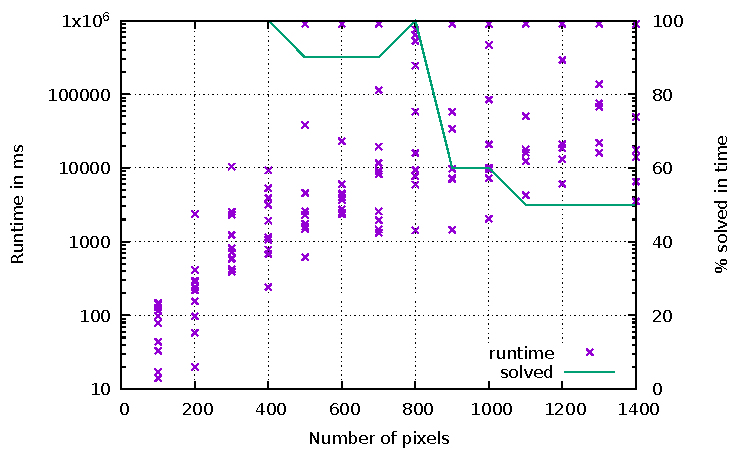
\includegraphics[width=\columnwidth]{icra2018/runtime_cc_optimal_random.pdf}
%	\caption{Runtime of solving benchmark instances to optimality. Shown
%	are the times of ten instances for each size, with a timeout at \SI{900}{\second}, as
%well as the percentage of solved instances. Only the number of turns is minimized in these instances.} \label{fig:experimentsfromthesis}
%\vspace{-1em}
%\end{figure}
%
%We evaluated the effectiveness of our optimization method by testing it on a suite of benchmark instances based on
%random natural grid graphs with random densities; %corresponding to the setting of mosquito distributions,
%the probability of a pixel to be added during test instance generation is correlated with its neighborhood, resulting in smoother boundaries which are more natural than purely random instances.
%% Changed the sentence above. It didn't make any sense to me.
%The tests were carried out for \num{10} instances for each size in the range up to \num{1400} pixels. 
%We used modern desktop computers equipped with an \emph{Intel(R) 
%Core(TM) i7-6700K CPU @ \SI{4.00}{\giga\Hz}} and \SI{64}{\giga\byte} of RAM. The integer programs were computed with CPLEX version 12.5.0.0 
%and the parameters \texttt{EpInt=0}, \texttt{ EpGap=0}, \texttt{ EpOpt=1e-9}, and \texttt{ EpAGap=0}.
%Fig.~\ref{fig:experimentsfromthesis} shows runtimes for solving penalty cycle cover to optimality. 
%Instances that took longer than \SI{15}{\minute} were aborted.
%As shown in the figure, 
%even at \num{1400} pixels we were still able to solve half of the instances to provable optimality.
%Even for the aborted instances, the computed solutions were within a few percentage points of
%the provable lower bound, meaning that they were nearly optimal.
%
%%PC stats, copied from thesis.
%
%Fig.~\ref{fig:ipexample} shows an example of iteratively computing an optimal tour with the described integer program.
%This example took less than a minute of total computing time.
%It assumed that $90^\circ$ turns cost five times as much as a straight pixel transition (distance).
%%but other instances are much more problematic. %such that selecting and connecting a subset of cycles instead of separating the integer program is more practical.
%
%\begin{figure}
%	
\includegraphics[width=0.24\columnwidth]{icra2018/ip_density}
%	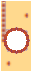
\includegraphics[width=0.24\columnwidth]{icra2018/ip_density_r_1}
%	
\includegraphics[width=0.24\columnwidth]{icra2018/ip_density_r_2}
%	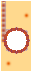
\includegraphics[width=0.24\columnwidth]{icra2018/ip_density_r_3}
%	\caption{Left is an optimal penalty cycle cover. Cycles (blue) cover all areas with high density. After three applications of the tour constraints, a single cycle remains (right). In the intermediate solutions, the subcycles first try to evade the new constraints by reshaping. The final tour omits two of the small hotspots because the cost of integrating them into the single 
%tour is prohibitively expensive.}
%\vspace{-1em}
%	\label{fig:ipexample}
%\end{figure}

\section[Experiments]{Experiments}

The results for representative flights are described below. Figure \ref{fig:fountain} compares the energy consumption for three coverage schemes for a region including a large obstacle in the center.  
A boustrophedon path requires 50 turns, $\SI{187}{\kilo\joule}$, $\SI{160}{\second}$, and $\SI{181}{\metre}$.
A hand-designed path requires 45 turns, $\SI{214}{\kilo\joule}$, $\SI{155}{\second}$, and $\SI{178}{\metre}$.
A path computed using the optimal penalty cycle cover requires only 33 turns, $\SI{184}{\kilo\joule}$, $\SI{133}{\second}$, and $\SI{176}{\metre}$.

\begin{figure}[h]
	\begin{center}
	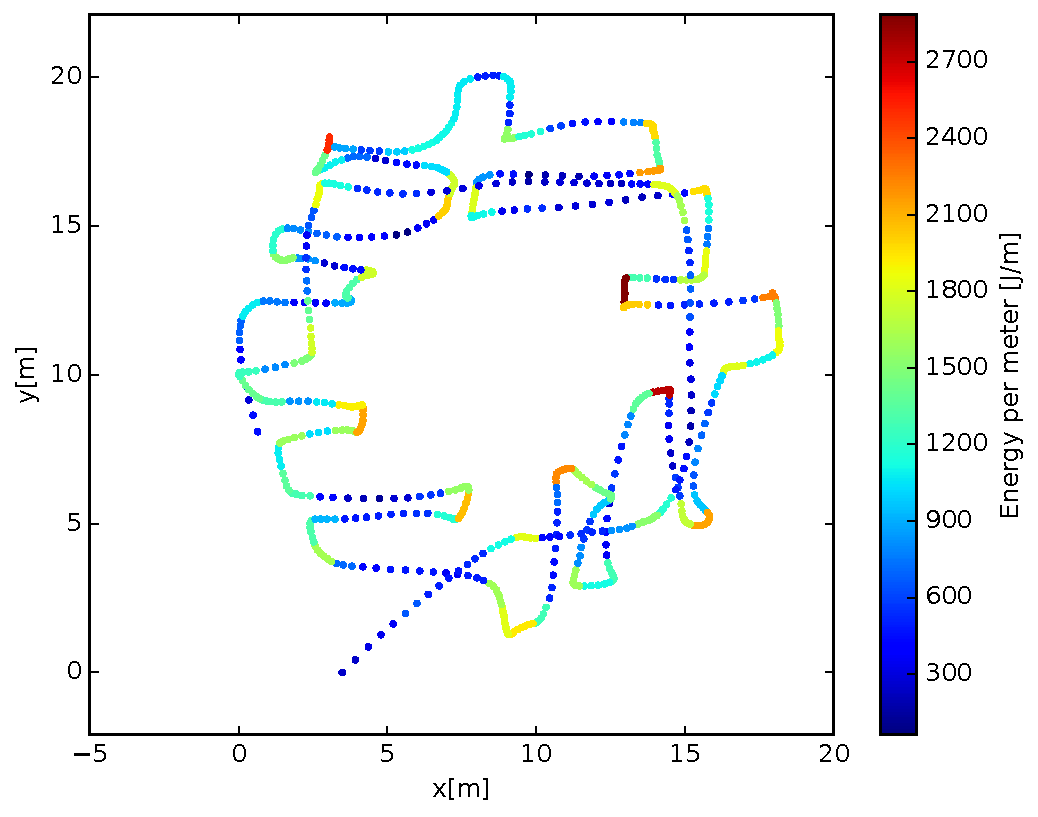
\includegraphics[width=.48\columnwidth]{icra2018/energy_path_2-notype3}
	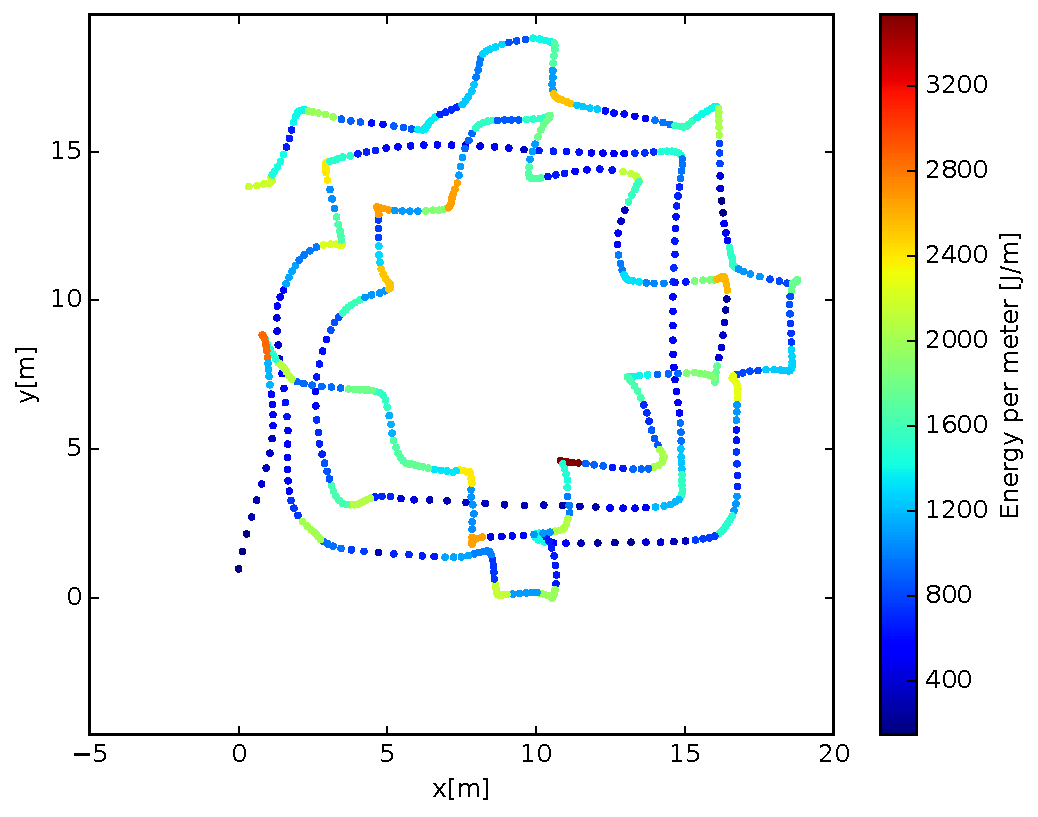
\includegraphics[width=.48\columnwidth]{icra2018/energy_path_3-notype3}
	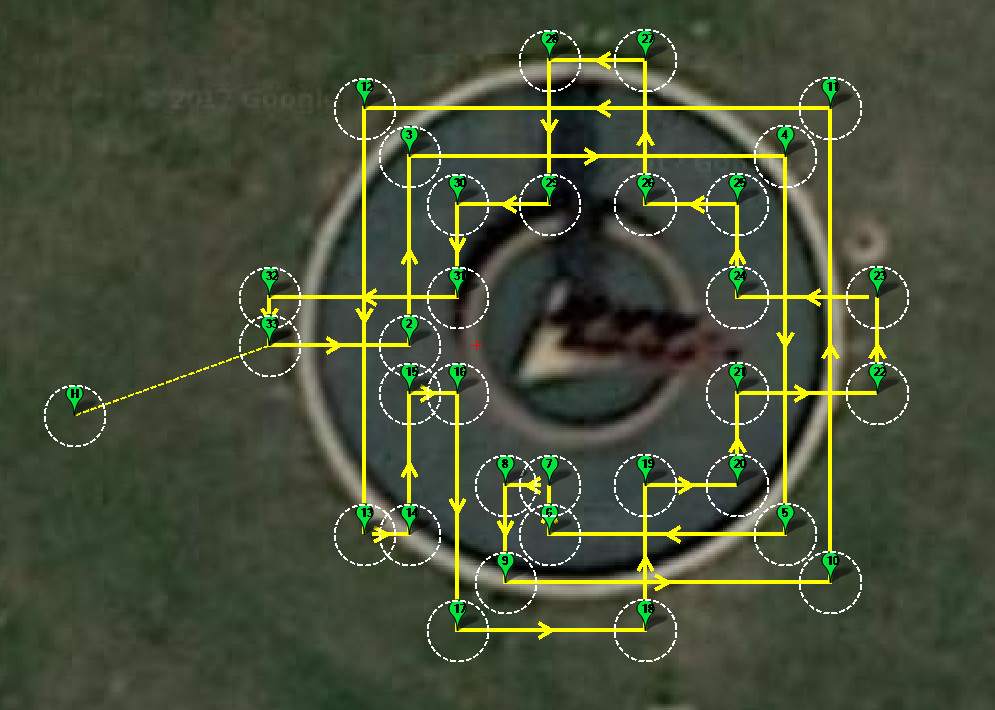
\includegraphics[width=.48\columnwidth]{icra2018/turncost_180}
	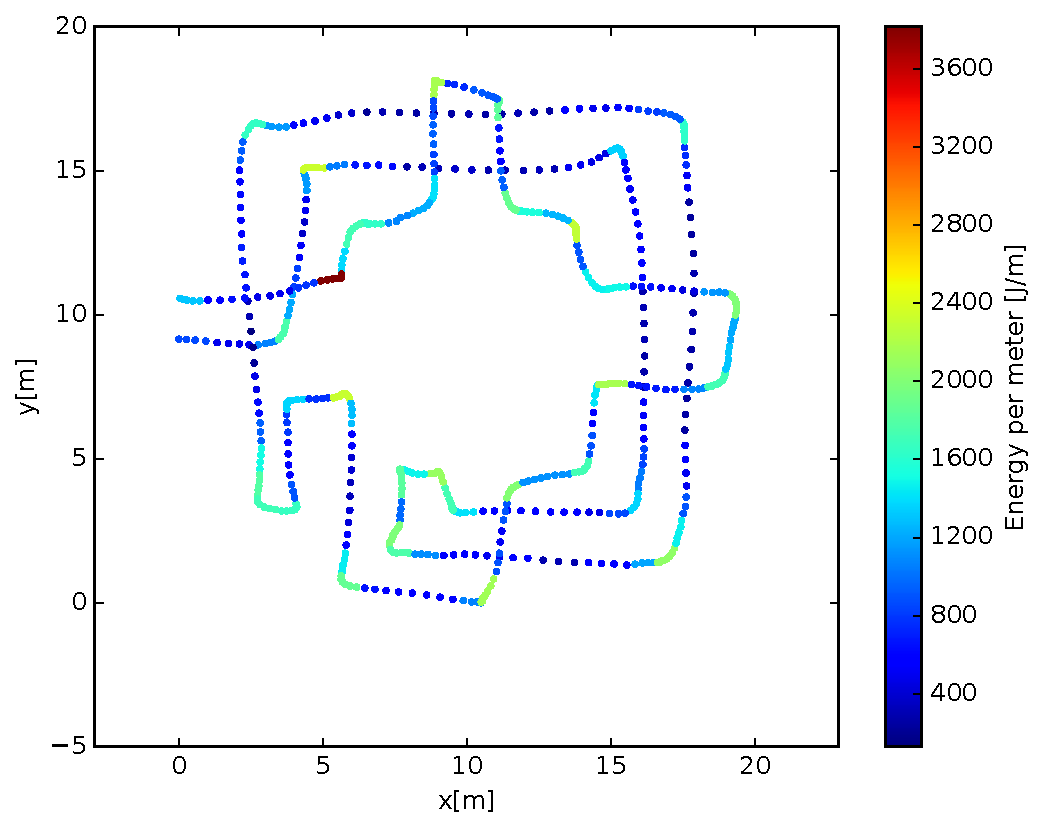
\includegraphics[width=.48\columnwidth]{icra2018/energy_path_1}
	\caption[Fountain]{Paths for an environment surrounding a fountain, which poses an obstacle for the UAV. 
	(Top left) The energy consumption during a real world flight for a boustrophedon path.
	(Top right) The energy consumption during a real world flight for a hand-designed loop path.
	(Bottom left) The optimal penalty cycle cover path.
	(Bottom right) The energy consumption during a real-world flight along the optimal path.} \label{fig:fountain}
	\end{center}
	\vspace{-1em}
\end{figure}


A boustrophedon (back-and-forth) path with \SI{2}{\metre} spacing was generated to cover a region $\SI{120}{\metre} \times \SI{15}{\metre}$ at height $\SI{1.5}{\metre}$.
The path was generated using Mission Planner software from ardupilot.org~\cite{Ardupilot}.

For each trial the UAV took off from a resting position on top of the screen.
Flight began manually, with a piloted takeoff of the UAV. After establishing a stable hover at $\SI{3}{\metre}$, control was switched to the autonomous flight plan.
The pilot monitored the flight with the ability to switch to manual operation in case of potential crashes due to GPS error or hazards in the flight plan.
Mosquito strikes detected by the data logger were verified using a GoPro Hero 4 Silver camera attached at the top of the net, as shown in Fig.~\ref{fig:DroneAndNet}.
At night and twilight, the sparks could be detected both visually and audibly from the recorded video.
During the day, the sparks were loud enough to observe over the audio channel of the videos.

The UAV flew eight missions on this field, covering the same path.
It was mainly flown in the early morning and late afternoon, when mosquito activities are more active.
Three flights were flown at noon and early afternoon to ensure that mosquito activities during these periods were not ignored.
However, only two mosquito strikes were observed during this period.
The path covered is about $\SI{1}{\kilo\metre}$ long and typically takes $\SI{12}{\minute}$.

Over the eight missions on this field, there were a total of 11 mosquito strikes.
Figure \ref{fig:strikemap} shows the mission's flight path and the map of all collected strikes.
The mosquito strikes are concentrated at the north and south ends of the field, where there are more trees.
A density map was generated from the collected strikes' position by representing each strike by a Gaussian distribution with the norm on the strike's location and a $\sigma$ of $\SI{10}{\metre}$.
Figure \ref{fig:densitymap} shows the density map generated by summing these Gaussian distributions.

\begin{figure}
	\centering
	\begin{overpic}[width=1.0\columnwidth]{icra2018/strikeMap.png}\end{overpic}
	\caption{\label{fig:strikemap}
	The UAV's path for flight 3 is in red. Strikes collected along this path are represented by yellow dots.} 
\end{figure}


\begin{figure}
	\centering
	\begin{overpic}[width=1.0\columnwidth]{icra2018/densityMap.pdf}\end{overpic}
	\caption{\label{fig:densitymap} Density map showing mosquito distribution on the field, overlaid by flight path 4 in white. 
	} \vspace{-2em}
\end{figure}

These results not only tell where mosquitoes were but also show where mosquitoes were not.
This is a key difference from stationary traps such as~\cite{chen2014flying,linn2016building}.
Figure~\ref{fig:DroneAndNetOutside} shows the UAV during a dawn flight test near the ocean.    

\begin{figure}
	\centering
	\begin{overpic}[width=1.0\columnwidth]{icra2018/OutdoorMosquitoDrone.jpg}\end{overpic}
	\caption{\label{fig:DroneAndNetOutside}
	The UAV and screen during a flight trial near the ocean.
	} 
\end{figure}


\section{Conclusion and Future Work}\label{sec:conclusion}

This chapter presented an approach for finding optimal tours given turn costs and an energy budget, inspired by a mosquito-killing UAV with limited battery life. 
Initial experiments with the UAV and electrified screen track the location of a mosquito-killing UAV as it patrols a field and maps mosquito kills.  

%Future work
Many refinements to the algorithm could be pursued in future work, including changes to both the mosquito-biasing algorithm and the robot flight simulation.  The model may be expanded to continuous space, three dimensions, and to arbitrary turn angles.  These and other considerations will make a more realistic model for future work.  

Further testing of the multi-copter UAV is indicated and will allow more extensive testing of the robustness and accuracy of the hardware design. New sensors that can identify and detect flying insects~\cite{chen2014flying} may be added to the UAV and enable it to proactively steer toward insect swarms and identify insects in realtime.

The concept may be extended to a non-destructive population survey in which the screen could be replaced with a net and, with appropriate lighting, the camera used to record capture events.  Teams of UAVs could work together to map areas more quickly and, by measuring gradients of the distribution, quickly find large mosquito populations.



%%  links for ICRA 2016, 
%%     to submit https://ras.papercept.net
%%     to test pdf
%%  compress using: gs -sDEVICE=pdfwrite -dCompatibilityLevel=1.4 -dNOPAUSE -dQUIET -dBATCH      -sOutputFile=MosquitoUAVcompressed.pdf MosquitoDroneICRA2018.pdf
%
%\documentclass[letterpaper, 10 pt, conference]{ieeeconf}  % Comment this line out if you need a4paper
%%\documentclass[a4paper, 10pt, conference]{ieeeconf}      % Use this line for a4 paper
%\pdfminorversion=4              % tell pdflatex to generate PDF in version 1.4
%\IEEEoverridecommandlockouts                              % This command is only needed if 
%                                                          % you want to use the \thanks command
%
%\overrideIEEEmargins                                      % Needed to meet printer requirements.
%
%% See the \addtolength command later in the file to balance the column lengths
%% on the last page of the document
%
%% The following packages can be found on http:\\www.ctan.org
%%\usepackage{graphics} % for pdf, bitmapped graphics files
%%\usepackage{epsfig} % for postscript graphics files
%%\usepackage{mathptmx} % assumes new font selection scheme installed
%%\usepackage{times} % assumes new font selection scheme installed
%%\usepackage{amsmath} % assumes amsmath package installed
%\usepackage{amssymb}  % assumes amsmath package installed
%\usepackage{mathtools,cuted}
%\usepackage{overpic}
%\graphicspath{{./pictures/},{./pictures/pdf/},{./pictures/ps/},{./pictures/png/},{./pictures/jpg/}}
%\usepackage{amsmath}
%\usepackage[table,xcdraw]{xcolor}
%\usepackage[hidelinks]{hyperref}
%\usepackage{flushend}
%\newcommand{\todo}[1]{\vspace{5 mm}\par \noindent \framebox{\begin{minipage}[c]{0.98 \columnwidth} \ttfamily\flushleft \textcolor{red}{#1}\end{minipage}}\vspace{5 mm}\par}
%
%%units
%\usepackage[per-mode=symbol, detect-weight=true, binary-units=true]{siunitx}
%
%\title{\LARGE \bf
%Using a UAV for Destructive Surveys of Mosquito Population
%}
%
%
%\author{An Nguyen, Dominik~Krupke, Mary Burbage, Shriya Bhatnagar, S{\'a}ndor~P.~Fekete, and Aaron T. Becker% <-this % stops a space
%\thanks{*This work was supported by the National Science Foundation under Grant No.\ \href{http://nsf.gov/awardsearch/showAward?AWD_ID=1553063}{ [IIS-1553063]} and \href{https://nsf.gov/awardsearch/showAward?AWD_ID=1646607}{[IIS-1646607]}.}
%\thanks{A. Nguyen, M. Burbage, S. Bhatnagar, and A. Becker are with the ECE Department at the University of Houston, TX.
%        \protect\url{an.nguyen.vn@ieee.org, atbecker@uh.edu}.
%        S.~Fekete and D.~Krupke are with the Dept.~of Computer Science, TU Braunschweig, Germany,
%      \protect\url{s.fekete@tu-bs.de, d.krupke@tu-bs.de  }
%        }%
%}
%
%\begin{document}
%
%\maketitle
%\thispagestyle{empty}
%\pagestyle{empty}
%
%
%%%%%%%%%%%%%%%%%%%%%%%%%%%%%%%%%%%%%%%%%%%%%%%%%%%%%%%%%%%%%%%%%%%%%%%%%%%%%%%%%
%\begin{abstract}
%This paper introduces techniques for mosquito population surveys in the field using electrified screens (bug zappers) mounted to a UAV. Instrumentation on the UAV logs the UAV path and the GPS location, altitude, and time of each mosquito elimination. 
%Hardware experiments with a UAV equipped with an electrified screen provide real-time measurements of (former) mosquito locations and mosquito-free volumes.
%Planning a trajectory for the UAV that maximizes the number of mosquito kills is related to the Traveling Salesman Problem, the Lawn Mower Problem and, most closely, Milling with Turn Cost. 
%We reduce this problem to considering variants of covering a grid graph with minimum turn cost, corresponding
%to optimized energy consumption. 
%We describe an exact method based on Integer Programming that is able to compute provably optimal instances with over 1,500 pixels. 
%These solutions are then implemented on the UAV.
%\end{abstract}
%
%%%%%%%%%%%%%%%%%%%%%%%%%%%%%%%%%%%%%%%%%%%%%%%%%%%%%%%%%%%%%%%%%%%%%%%%%%%%%%%%%
%
%
%\section{Introduction}
%
%Mosquito-borne diseases kill millions of humans each year~\cite{murray2012global}. 
% Because of this threat, governments worldwide track mosquito populations.
% Tracking individual mosquitoes is difficult because of their small size, wide-ranging flight, and preference for low-light.
% Tracking studies of individual mosquitos have chosen to use small ($\SI{1.2}{\metre} \times \SI{2.4}{\metre}$) indoor regions~\cite{parker2015infrared}, or mating swarms backlit against a solid background~\cite{butail20113d}.
%
%The dominant tools for tracking mosquito populations are stationary traps that are checked at weekly intervals (\textit{e.g.} Encephalitis Vector Surveillance traps and/or gravid traps~\cite{williams2007comparison}). 
%Recent research has focused on making these traps smaller, cheaper, and capable of providing real-time data~\cite{chen2014flying,linn2016building}; however, they still rely on attracting mosquitoes to the trap. 
% This paper presents an alternate solution using an electrified bug-zapping screen mounted on an unmanned aerial vehicle (UAV) as shown in Fig.~\ref{fig:DroneAndNet} to seek out the mosquitoes in their habitat.  As the UAV follows a path, it sweeps out a volume of air, temporarily removing all the mosquitoes in this volume.  By monitoring the voltage across this screen, we can track individual mosquito contacts.
%     UAVs have strict energy budgets, so optimized flight patterns are of crucial importance. As a consequence, putting
%the UAV to good use requires
%methods for computing trajectories that minimize energy consumption along the way, but maximize the total volume of mosquitoes 
%at visited locations.
%
%%the available flight time depends on the flight pattern, as making it crucial to optimize the used trajectories. As it turns out, threquires the utility of a which makes it necessary to  which limit the flight time to a maximum denoted by $T$.
%    %The goal is to design a trajectory for the mosquito screen with duration less than $T$ that maximizes the number of mosquito eliminations.
%
%  \begin{figure}
%\centering
%\begin{overpic}[width=1\columnwidth]{DroneAndNet_v2.pdf}\end{overpic}
%\caption{\label{fig:DroneAndNet}
%	  A hexacopter UAV carrying a $\SI{48}{\centi\metre} \times \SI{61}{\centi\metre}$ rectangular bug-zapping screen. An onboard micro controller monitors the voltage across the screen and records the time, GPS location, humidity, and altitude for each mosquito strike.  At right are three frames recorded by the onboard camera showing mosquito hits, during the day (top) and at twilight.
%See attachment for videos of flight experiments~\cite{Bhatnagar2018}.
%%Video is available at \href{https://youtu.be/1gvJ-yTf-E8}{https://youtu.be/1gvJ-yTf-E8}~\cite{DroneVideo}. 
%\vspace{-2em}
%}
%\end{figure}
%
%
%   % This process can be modeled as sampling without replacement from a point cloud of mobile particles using a mobile agent.  The point cloud particles are generated from a known or unknown distribution, and the mobile agent clears all particles in a swept-out region each time step. 
%%    UAVs have strict energy budgets, which limit the flight time to a maximum denoted by $T$.
%%    The goal is to design a trajectory for the mosquito screen with duration less than $T$ that maximizes the number of mosquito eliminations.%, in probability, samples the most particles.  
%%   We assume the agent can detect each particle collision and can use these detections to modify a planned trajectory.
%%    This paper presents both open-loop trajectories and policies with feedback. 
%%  
%%      \subsection{Overview}
%%A multimedia introduction to the techniques used in this paper is available at~\cite{becker2017zapping}.
%  This paper is arranged as follows.  
%  After a review of related work in \S \ref{sec:relatedWork}, 
%  we describe a design and rationale for a UAV with bug zapper in \S  \ref{Sec:HardwareDesign}.
%    We next present a path planning optimization strategy in   \S \ref{sec:Simulation}.
%  We then describe hardware experiments with the UAV  in \S  \ref{sec:Experiments} and conclude with directions for future research  in \S  \ref{sec:conclusion}.
%  
%  
% 
%
%%%%%%%%%%%%%%%%%%%%%%%%%%%%%%
%  \section{Related Work}\label{sec:relatedWork}
%%%%%%%%%%%%%%%%%%%%%%%%%%%%%%  
%  \noindent \emph{Robotic Coverage}: 
%    Robotic coverage has a long history. The basic problem is one of designing a path for a robot that ensures the robot visits within $r$ distance of every point on the workspace.  For an overview see~\cite{Choset2001}.  This work has been extended to use multiple coverage robots in a variety of ways, including using simple behaviors for the robots~\cite{spears2006physics,Koenig2001}.
%%This is closely related to the art gallery problem~\cite{lee1986computational} but with limited range of visibility.
% %   The key difference in the mosquito coverage problem is that the mosquitoes can move, recontaminating an area previously cleared. We instead have a probability of coverage, as in~\cite{Das2011}.  
%    
%\noindent  \emph{Mosquito Control Solutions}:
%	Mosquito control also has a long history of efforts associated both with monitoring mosquito populations~\cite{dennett2007associations} and with eliminating mosquitoes.  The work involves both draining potential breeding grounds and destroying living mosquitoes~\cite{peter2005tick}.  An array of insecticidal compounds has been used with different application methods, concentrations, and quantities, including both larvicides and compounds directed at adult mosquitoes~\cite{larvicides2005guidelines}.
%	
%	Various traps have been designed to capture and/or kill mosquitoes with increasing sophistication in imitating human bait, as designers strive to achieve a trap that can rival the attraction of a live human~\cite{maliti2015development}.  In recent history, methods have also included genetically modifying mosquitoes so that they either cannot reproduce effectively or cannot transmit diseases successfully~\cite{marshall2009malaria}, and with the recent genomic mapping of mosquito species, new ideas for more targeted work have been formulated~\cite{hill2005arthropod}.
%	
%	Popular methods to control mosquitoes such as insecticides are effective, but they have the potential to introduce long-term environmental damage and mosquitoes have demonstrated the ability to become resistant to pesticides~\cite{ndiath2012resistance}. Traditional electrified screens (bug zappers) use UV light to attract pests but have a large bycatch of non-pest insects~\cite{University-Of-Florida1997}. 
%%	This paper introduces techniques using bug zappers mounted on unmanned vehicles to autonomously seek %out and eliminate mosquitoes in their breeding grounds and swarms. Instrumentation on the bug zappers %logs the GPS location, altitude, weather details, and time of each mosquito hit.  Mosquito control %offices can use this information to analyze the insects' activities. The device can be mounted on a %remote-controlled or autonomous unmanned vehicle. If autonomous, the vehicle can use the data collected %from the electrified screen as feedback to improve the effectiveness of the motion plan. 
%	
%  \noindent  \emph{Robotic Pest Management}:
%As GPS technology has flourished and data processing has become cheaper and more readily available, researchers have explored options for implementing the new technologies in breeding ground removal~\cite{anupa2014identification} and more effective insecticide dispersion~\cite{hur2015low}.  Low-cost UAVs for residential spraying are under development~\cite{amenyo2014medizdroids}.  Even optical solutions have been considered, including laser containment~\cite{boonsri2012laser} or, by extension, exclusion and laser tracking and extermination~\cite{kare2010build}.
%    
%   
%    
%  \section{Hardware Design}\label{Sec:HardwareDesign}%%%%%%%%%%%%%%%%%%
%  %%%%%%%%%%%%%%%%%%%%%%%%%%%%%%%%%%%%%%%
%  This section examines the components of the mosquito UAV system, shown in Fig.~\ref{fig:DroneAndNet}. This includes the UAV, electrified screen, surveying electronics, and a discussion of the energy budget. 
% % The design for the mosquito UAV system been assigned a U.S.\ Provisional Patent Application~\cite{Becker2016patentapp}.
%  
%  \subsection{UAV}
%  
%The UAV is a custom-built, $\SI{177}{\centi\metre}$ wingspan hexacopter, controlled by a Pixhawk flight controller running ArduPilot Mega flight software. The UAV has a 3DR GPS module using the UBlox NEO-7 chipset.
%
%  \subsection{Screen Design}
%     The mosquito screen is designed to eliminate high density mosquito populations. 
%  This screen was constructed from two expanded aluminum mesh panels, spaced apart by \SI{3}{\milli\metre} thick ABS grid. 
%   These mesh panels have \SI{12}{\milli\metre} diamond-shaped  openings, and is held taught by nylon bolts around the perimeter.  
%   The bottom mesh panel is offset by half a diamond (6 mm) to the right to ensure all insects greater than 6 mm cannot pass through the net.
%     The top mesh is held at the reference voltage and the bottom mesh is energized to $1.8~kV$ above the reference voltage.
%     
%  The perimeter is reinforced by two sets of \SI{7}{\milli\metre} diameter fiberglass rods that are inset into 3D printed corner fixtures.
%  These rods protect the frame from getting damaged from any side, and allows the UAV to land without damaging the net.
%
%
%Once assembled, the net weighs \SI{0.948}{\kilogram} and has an overall area of \SI{0.194}{\square\metre}, with the spacer occupying \SI{0.0325}{\square\metre}. 
%This makes the effective net area \SI{0.161}{\square\metre}. %, and the total cost of building a net this size is only \$27.44 USD.
%   
%   
%
%  %Design files and build instructions are available at~\cite{Vinh2016BugNet}.
%
%
%  %%%%%%%%%%%%%%%%%%%%%%%
%  \subsection{Screen Location}
% The UAV carries the bug-zapping screen, which is suspended by paracord rope at each corner.  The location of this screen determines the efficacy of the mosquito UAV, measured in mosquitoes detected per second of flight time. The following describes a simplified analysis to optimize the screen location.
%
%For manufacturing ease, the electrified screen is a rectangle with a width of $d_s$. The screen is suspended a distance $h_s$ beneath the UAV flying at height $h_d$.  We chose to suspend the screen beneath the UAV to avoid the weight of the rigid frame that would be required if the screen were above the UAV and because most mosquito species prefer low flight~\cite{gillies1976vertical}.  This screen can be suspended at any desired angle $\theta$ in comparison to horizontal, as shown in Fig.~\ref{fig:DroneConfigs}.
%Two key parameters are the distance $h_s$ and the optimal angle $\theta$.  The goal is to clear the greatest volume of mosquitoes per second, a volume defined by the UAV forward velocity $v_f$ and the cross-sectional area $h_m \times d_s$ cleared by the screen, as shown in Fig.~\ref{fig:AngleVsSpeed}.
%
% To hover, the UAV must push sufficient air down with velocity $v_d$ to apply a force that cancels the pull of gravity.  The UAV and screen combined have mass $m_{d}$ and its cross section can be approximated as a square with a side length of $d_d$.  The mass flow of air through the UAV's propellers is equal to the product of the change in velocity of the air, the density of the air $\rho_a$, and the cross sectional area.
% 
%     \begin{figure}
%\centering
%\begin{overpic}[width=\columnwidth]{DroneConfigs.pdf}\end{overpic}
%\caption{\label{fig:DroneConfigs}
%The UAV suspends a rectangular bug-zapping screen beneath it.  Propwash pushes incoming mosquitoes downwards, and the UAV clears a volume $h_m \times d_s \times v_f$ each second. Circles show two mosquitoes at equal time intervals relative to the UAV.} 
%\vspace{-1em}
%\end{figure}
%
%
%We assume that air above the UAV is quiescent, so the change in velocity of the air is $v_d~ \si{\metre\per\second}$.
% \begin{align} \label{eq:forceBalanceForDrone}
% \text{Force gravity} & = \left(\text{mass flow}\right) \cdot \text{air velocity} \nonumber \\
% m_{d} \cdot  g &= (v_d \cdot  \rho_a \cdot  d_d^2 ) \cdot  v_d 
%% \text{kg} \cdot \frac{ \text{m}}{ \text{s}^2}&= \left( \frac{ \text{m}}{\text{s}} \cdot  \frac{ \text{kg}}{\text{m}^3}  \cdot \text{m}^2 \right) \cdot  \frac{ \text{m}}{\text{s}}\nonumber
%\end{align}
%
%Then the required \emph{propwash}, the velocity of air beneath the UAV, for hovering is
% \begin{align} \label{eq:dronePropwash}
%v_d = \sqrt{ \frac{ m_d g}{\rho_a d_d^2} }
%\end{align}
%The flight testing site in Houston, Texas is \SI{15}{\metre} above sea level. At sea level the density of air $\rho_a$ is \SI{1.225}{\kilogram\per\cubic\metre}.
%The UAV and instrumentation combined weigh \SI{5.1}{\kilogram} with a width of \SI{0.75}{\metre}. The acceleration due to gravity is \SI{9.871}{\metre\per\square\second}.  Substituting these values gives $v_d = \SI{8.5}{\metre\per\second}$.
%
%Due to propwash, an initially hovering mosquito will fall when under the UAV at a rate of $v_d$.  Relative to the UAV, the mosquito moves horizontally at a rate of $-v_f$.  As shown in Fig.~\ref{fig:DroneConfigs}, we can extend lines with slope $-v_d/v_f$ from the screen's trailing edge to $h_{\textrm{top}}$ and from the leading edge to $h_{\textrm{bottom}}$.
% \begin{align} \label{eq:ClearedCrossSection}
%h_{\textrm{top}} &= h_d - h_s + \frac{d_s}{2} \sin(\theta) +  \frac{d_d + d_s\cos(\theta)}{2}  \frac{v_d}{v_f} \nonumber \\
%h_{\textrm{bottom}} &= h_d - h_s - \frac{d_s}{2} \sin(\theta) +  \frac{d_d - d_s\cos(\theta)}{2}  \frac{v_d}{v_f}  \nonumber \\
%h_m &= h_{\textrm{top}} - h_{\textrm{bottom}} =  d_s\left(\frac{v_d}{v_f}\cos(\theta) + \sin(\theta) \right)
%\end{align}
%The optimal angle is therefore a function of forward and propwash velocity:
%\begin{align} \label{eq:OptimalScreenAngle}
%\ \theta = \mathrm{ArcTan}\left(\frac{v_f}{v_d}\right)
%\end{align}
%
%To ensure the maximum number of mosquitoes are collected, the screen must be sufficiently far below the UAV $ h_s > \frac{d_s}{2} \sin(\theta) +  \frac{d_d + d_s\cos(\theta)}{2}  \frac{v_d}{v_f}$  and the bottom of the screen must not touch the ground, $ h_d > h_s + \frac{d_s}{2} \sin(\theta) $.
%
%      \begin{figure}
%\centering
%\begin{overpic}[width=\columnwidth]{AngleVsSpeed.pdf}\end{overpic}
%\caption{\label{fig:AngleVsSpeed}
%The volume cleared by a UAV is a function of screen angle $\theta$ and forward velocity $v_f$.  Dotted line shows the optimal angle given in \eqref{eq:OptimalScreenAngle}. } 
%\vspace{-1em}
%\end{figure}
% 
%There are practical limits to $h_s$ as well.  Tests with $h_s > \SI{2}{\metre}$ were abandoned because the long length caused the screen to act as a pendulum, introducing dynamics that made the system difficult to fly.
% 
%Changing the flying height $h_d$ of the UAV will target different mosquito populations because mosquitoes are not distributed uniformly vertically. 
% Gillies and Wilkes demonstrated that different species of mosquitoes prefer to fly at different heights~\cite{gillies1976vertical}. 
% 
%   %%%%%%%%%%%%%%%%%%%%%%%
%   \subsection{Wind Tunnel Verification of Net Angle}
%   
%This section describes experiments run in a wind tunnel to verify the simplified net angle analysis in the previous section. 
%Smoke streaklines were used to visualize the flow of air as it passed by the UAV.
%Due to space constraints in the wind tunnel, a free-flying phantom 4 was used instead of the hexacopter used for carrying the zapper. 
%The wind tunnel was set to a \SI{3}{\metre\per\second} flow speed, and the UAV manually flown in approximately stable hovering.
%The solo UAV is \num{0.3} $\times$ \num{0.3} $\times$ \SI{0.2}{\metre}.  The windtunnel has a \SI{1}{\metre} $\times$ \SI{1}{\metre} cross section. 
%%??? brand name of the smoking apparatus?
%As seen from Fig.~\ref{fig:WindTunnel}, the proposed screen position captures free flowing air and air entrained by the UAV propellers.
%This test encouraged us to mount the net as close to the UAV as possible, so that air, and flying mosquitos, entrained by the propellers are pushed into the net.
% 
%
%\begin{figure}
%\centering
%\begin{overpic}[width=1.0\columnwidth]{WindTunnelv01lowres.pdf}\end{overpic}
%\caption{\label{fig:WindTunnel}
%	Frames from wind tunnel test with free-flying UAV at \SI{3}{\metre\per\second} windspeed with smoke for streaklines~\cite{Bhatnagar2018}.  As shown in the frames at right, the proposed screen position (in red) captures free flowing air and air entrained by the UAV propellers.
%	Each black square is \SI{25.4}{\milli\metre} in width.
%  } \vspace{-1em}
%\end{figure}
% 
%
%  %%%%%%%%%%%%%%%%%%%%%%%
%   \subsection{Data Logger}
%   
%   The electrical detection and logging system is powered by a $9~V$ lithium ion battery applied directly to the controller and two AA $3~V$ lithium ion batteries applied to the power circuit for the screen.
%   The controller uses a GPS shield for monitoring the location and altitude as well as a real time clock to timestamp each data point collected from the system.
%   A Raspberry Pi 3 is used for data logging, 
%       sensors include a GPS sensor (NEO-6M Ublox), 
%      a capacitive humidity sensor, a thermistor (DHT22),
%   %ADS1115 16-bit ADC for monitoring the supply-side voltage of the net, and 
%   and an INA219 high side, 12-bit DC current sensor for monitoring the supply-side current delivered to the net.
%   The net current draw is logged at 100 Hz, while GPS and weather sensor data is logged at 1Hz.  
%   All data is stored on an onboard SD card.
%
%  %%%%%%%%%%%%%%%%%%%%%%%
%  \subsection{Energy Budget}
%  
%                  \begin{figure}
%\centering
%\begin{overpic}[width=1.0\columnwidth]{OscilloscopeTrace.pdf}\end{overpic}
%\caption{\label{fig:BugZapTrace}
%					  Current, voltage, and power traces for five \textit{Culex quinquefasciatus} mosquitoes as each contacts the bug-zapping screen at $t=0$.  Contact causes a brief short that recovers in $\SI{160}{\milli\second}$.
%  } 
%  \vspace{-1em}
%\end{figure}
% % \todo{what is the new energy usage of the screen?}
%  
%  
%  Tests with an oscilloscope show that in the steady state, a $\SI{30.5}{\centi\metre} \times \SI{61}{\centi\metre}$ screen and electronics have a power consumption of \SI{3.6}{\watt}.  During a zap, the screen voltage monitoring circuit shorts briefly when the mosquito contacts the screen.  Figure~\ref{fig:BugZapTrace} shows the time sequences for battery and screen voltages, current, and power during five mosquito zaps.  
%% % WE COULD NOT JUSTIFY THIS EQUATION 
%%%  The initial current spike recovery can be modeled with an exponential fit.
%%%
%% \begin{align} \label{eq:BugZapFit}
%%i=69.1e^{-2.7\times10^4 t} ~A
%%\end{align}
%%%
%%The fit in \eqref{eq:BugZapFit} gives a time constant of $36~\mu s$ for the short and a recovery time of $80~\mu s$. 
% Multiplying voltage by current to find the instantaneous power ($p=iv$) and integrating the area under the power curve show a total energy consumption of \SI{4.2}{\milli\joule} for each zap.  Recharging the screen requires more power and is represented in the latter part of the curves.  The overall recovery time is about $\SI{160}{\milli\second}$.  Most of the energy is consumed charging and maintaining the charge on the screen rather than in zapping the mosquitoes.
%  
%  
%
%
%
%%Data
%%The files used for this run of simulations are as follows:
%%MosquitoFlightSimv2p0.m
%%MosquitoSimv2p2randombounce.m
%%MosquitoSimv2p2boustrophedon.m
%%MosquitoSimComparev1p0.m
%%
%%All are located in the Dropbox code folder.
%%Raw data are located in the Excel file Simulation Results.xlsx.
%%    
%    
%%%%%%%%%%%%%%%%%%%
%%%%%%%%%%%%%%%%%%%%%%%%%%%%%%%%%%%%%%% 
\section[Path Planning]{Planning minimal turn cost paths}
%%%%%%%%%%%%%%%%%%%%%%%%%%%%%  

\newcommand{\revised}[1]{{\color{red}#1}}

%The following section present an overview of the algorithm used in the paper's research, which was done by our collaborators in Germany:
%D. Krupke and S.P. Fekete of TU Braunsweig.

\subsection{Modelling Mosquito Density}
\label{subsec:modelling}
Due to a-priori knowledge of mosquitos' preferred habitats from entomology, we can model the density of mosqitos in a field we want to cover.
This knowledge will help us plan the most efficient path, killing the most mosquitos with the least amount of energy used.
First, we divide a field for coverage into a pixel grid, the size of each pixel dictated by the size of the net and the resoultion of the UAV's GPS.
Each pixel $p_i\in P$ we give a relative density value $c(p_i)$ that describes the estimated mosquito density based on the environmental factor of the pixel.
In $P$ there will only be a subet with high relative density value.
The goal is to maximize the density covered by the set $S\subseteq P$ of visited pixels i.e., $\max_{S\subseteq P} \sum_{p_i\in S} c(p_i)$ within the available battery capacity.
This could be done in one single trip or over multiple trips with multiple batteries.

%The data on the distribution of mosquitoes is given for a two-dimensional grid environment; the grid size
%is induced by the size of the screen, the available data and the desired resolution of the extracted map. 
%For each pixel $p_i\in P$, we are given a relative value
%$c(p_i)$ that describes the estimated a-priori density of mosquitoes, based on data obtained from boustrophedon (back and forth) scans of the area by the UAV;
%this implies that only a subset of pixels carry a significant value.
%Visiting one of the pixels corresponds to sampling and mapping the actual density distribution of mosquitoes. 
%For a dense distribution of mosquitoes
%(which is the case for the instances relevant for pest control), multiple visits to the same pixel do not contribute additional
%knowledge. As a consequence, the objective is to maximize the sampling value of the set $S\subseteq P$ of visited pixels, 
%i.e., $\max_{S\subseteq P} \sum_{p_i\in S} c(p_i)$ {within the available battery capacity}; this may be over the course of a single closed trajectory, or over
%a combination of multiple roundtrips. 

\subsection{Turn Cost}

\begin{figure}[h]
\begin{center}
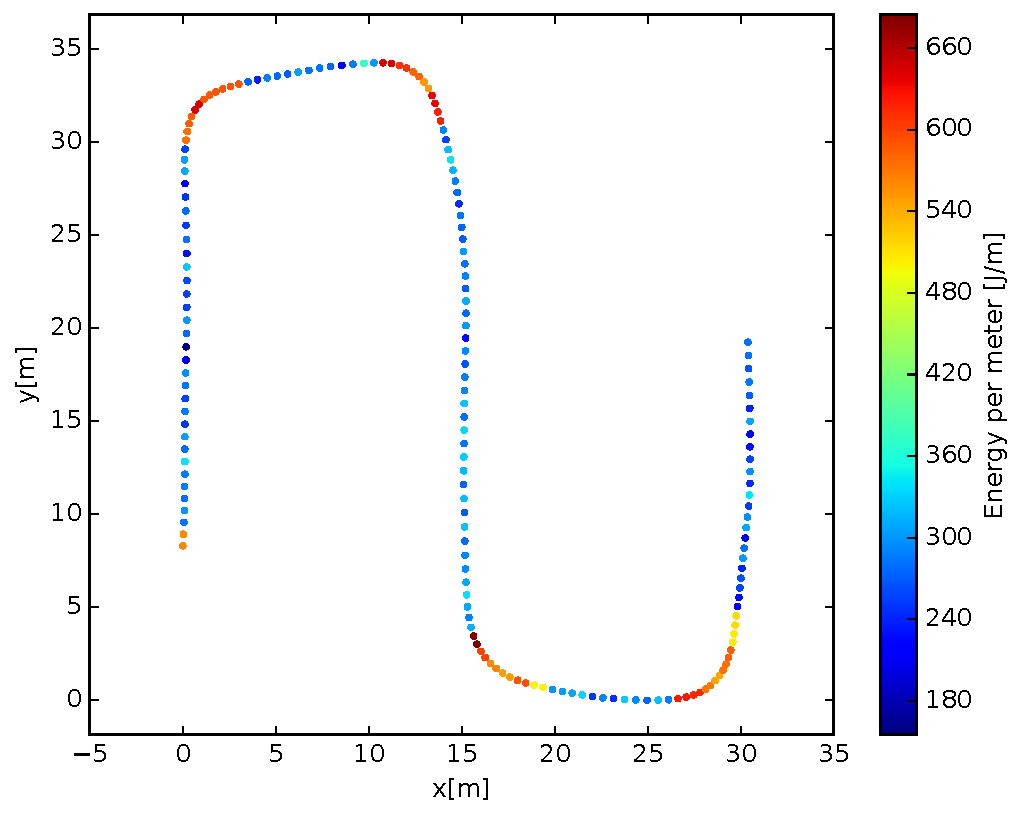
\includegraphics[width=.75\columnwidth]{icra2018/turncost}
\caption[Mosquito hunting drone]{Turns are expensive. See our related video at
\url{https://youtu.be/SFyOMDgdNao} for details, and
\cite{becker2017zapping} for an accompanying abstract.} \label{fig:turncost}
\end{center}
\vspace{-1em}
\end{figure}

UAVs can make turns on the spot, without curvature constraints like a fix-winged aircraft.
However, UAVs turns are energtically expensive.
As Fig.~\ref{fig:turncost} shows, the energy required per meter of travel in a turn is 4 to 5 times as expensive as traveling through a straight path.
The limiting factor for a UAV's flight is its battery capacity, therefor it is important to limit the amount of turns needed per flight while maximizing the amount of pixels visited.
To consider the total energy cost of a turn, we need to limit the types of turns the UAV made.
We consider only strict set of \ang{90} and \ang{180} turns since the UAV does not have minimal turn curvature.
Additionally, the two turn angles allow us to fly around most large obstacles while visiting the pixels around it.

%Planning good trajectories for a UAV is not subject to the same curvature constraints of an ordinary aircraft
%because UAVs can turn on the spot. However, turns are a critical aspect of path
%planning due to their impact on energy consumption.  Battery capacity is {\em the} limiting factor for  UAV flight time. As shown in Fig.~\ref{fig:turncost}, 
%the power output for a desired trajectory is non-uniform.  Flying along a straight path
%is relatively inexpensive but turning is energy intensive. 

%As a consequence, we must consider the total turn costs associated
%with changing direction, as measured by the turn angle.
%As we are not limited by trajectory curvature, we refer to straight-line connections and a finite set of $2\omega$ different
%headings for visiting vertices. For the most natural case of orthogonal grids $\omega=2$. When
%surveying non-isolated mosquito hotspots (whose size greatly exceeds the size of the UAV), we are not dealing with
%isolated pixels and the modeling error of this restriction is small.

%TODO: I guess one can save space here by e.g. skipping subset cover.
%Now we consider different trajectory types.
%A {\em cycle} is a roundtrip of a subset $S\subseteq P$ that visits all points in $S$ and returns to the origin, a {\em cycle cover} of $P$ is a set of cycles
%that together visit all points in $P$, and a {\em tour} is a single cycle that visits all points in $P$. A {\em subset cycle cover} for $S\subset P$ is a cycle
%cover that covers at least the points in $S$, while a {\em subset tour} is a tour of at least the points in $S$. For any of these structures, we are interested in
%%cycle covers or tours of {\em minimum total turn cost}. 
%{cycle covers or tours of {\em minimum total travel cost}. 
%The travel/battery cost is a linear combination of the number of pixel transitions (distance) and the weighted number of turns, 
%corresponding to the total turn angle.
%}
%In addition, a {\em minimum turn-cost penalty cycle cover}  or a {\em minimum turn-cost penalty tour}
%visits a subset $R\subset P$, such that the sum of total travel cost and the sum $\sum_{i\not\in R} c(p_i)$ of values of 
%unvisited pixels is minimized. 
%The travel/battery cost is a linear combination of the number of pixel transitions (distance) and the weighted number of turns, 
%corresponding to the total turn angle.
%Note that the travel cost
%may be a linear combination of turn and travel cost, as long as triangle inequality is satisfied.

%\subsection{Computational Complexity}
%\label{subsec:complexity}
%Finding optimal covering paths that map a given region is closely related to the famous 
%\emph{Traveling Salesman Problem (TSP)}, which asks to minimize
%total length of a single tour that covers all of a given set of locations. The TSP is one of 
%the classic NP-hard problems, so we cannot expect a general method that finds
%a provably optimal solution for any  instance in polynomially bounded time.
%A generalization of the TSP is
%the \emph{Lawnmower Problem} (see Arkin et al.~\cite{arkin2000approximation}, which considers coverage by
%a tool of nontrivial size. For the objective of minimizing the total cost (in particular, the turn
%cost), Arkin et al.~\cite{arkin2005optimal} showed that finding minimum-turn tours in grid graphs is NP-hard,
%even if a minimum-turn cycle cover is given. The complexity of finding a set of multiple cycles that cover a 
%given set of locations at minimum total turn cost had remained elusive for many years; \emph{Problem~{53}} in \emph{The Open Problems Project}
%%edited by Demaine, Mitchell, and O'Rourke~\cite{openproblemproject}
%asks for the complexity of finding a minimum-cost (full) cycle cover in a 2-dimensional grid graph. This is not 
%obvious: large parts of a solution can usually easily be deduced by local information and 2-factor techniques.
%Arkin et al. showed~\cite{arkin2005optimal,arkin2001optimal} that the full coverage variant in {\em thin} grid graphs (which do not contain a $2\times 2$ square,
%so every pixel is a boundary pixel) is solvable in polynomial time. In separate work~\cite{dom3}, two of us were able to resolve this
%issue by showing that finding a cycle cover of minimum turn cost is  NP-hard.

%\subsection{Mathematical Optimization}
%\label{subsec:complexity}
%A powerful approach for finding optimal solutions to instances of NP-hard problems is the use
%of Integer Programming (IP). While solving an IP still requires exponential time in the worst case,
%using carefully crafted mathematical models in combination with specific algorithm engineering and available
%IP solvers enables solving instances of considerable size to provable optimality.
%For our purposes, we can describe the problem as follows. 
%
%\paragraph{Penalty Cycle Covers}
%The set $P$ of pixels corresponds to a given grid graph $G(P,E)$ in which each pixel $p_j\in P$ is adjacent to the set $N(p_j)$
%of pixels in $P$ that share an edge with $p_j$.
%Each vertex $p_j\in P$ has a scalar reward $c(p_j)$ for visiting (or penalty for not visiting), 
%and a function $\text{cost}_j(i,k)\in \mathbb{Z}^+_0$  that maps the cost of traveling from $p_i$ to $p_j$ to $p_k$, where  $p_i,p_k\in N(p_j)$ are adjacent pixels to   $p_j$.
%This cost is symmetric, i.e. $\text{cost}_j(i,k)=\text{cost}_j(k,i)$. %TODO: Or cost(ijk) or cost(i,j,k) or cost(p_i, p_j, p_k)
%The integer program uses two types of variables: integer variables
%$x_{ijk}=x_{kji}$ that state how often passage $p_i-p_j-p_k$ or $p_k-p_j-p_i$ is used and
%Boolean variables $y_{j}$ that indicate that the pixel $p_j\in V$ is not covered,
%i.e., the penalty is paid.  This results in the following formulation: 
%%IP Formulation TODO
%%\begin{strip}
%%\begin{eqnarray}
%%	\min & \displaystyle  \sum_{p_j\in P} \sum_{p_i,p_k\in N(p_j)} \text{cost}_j(i,k) \cdot x_{ijk} + \sum_{p_j\in P}c(p_j) \cdot y_j\label{eq:obj}\\
%%	\text{s.t.}			& 1\leq\displaystyle 4 \cdot y_j +\sum_{p_i,p_k\in N(p_j)} x_{ijk} \leq 4&\forall p_j\in P \label{eq:ip:constr1}\\
%%						& \displaystyle 2 \cdot x_{jij} +\sum_{p_k\in N(p_i), p_k\not= p_j}x_{jik} = 2 \cdot x_{iji}+\sum_{p_k\in N(p_j), p_k\not= p_i}x_{ijk}  & \forall \{p_i,p_j\}\in E \label{eq:ip:constr2}\\
%%						& x_{ijk}\in\mathbb{N}_0, y_j\in \mathbb{B} & \forall p_j\in P, \{p_i,p_k\}\subseteq N(p_j)
%%\end{eqnarray}
%%\end{strip}
%\begin{eqnarray}
%	\min  \displaystyle  \sum_{p_j\in P} \sum_{p_i,p_k\in N(p_j)} \text{cost}_j(i,k) \cdot x_{ijk} + \sum_{p_j\in P}c(p_j) \cdot y_j\label{eq:obj}
%\end{eqnarray}
%with constraints
%\begin{eqnarray}
%	 1\leq\displaystyle 4 \cdot y_j +\sum_{p_i,p_k\in N(p_j)} x_{ijk} \leq 4, &\forall p_j\in P \label{eq:ip:constr1}
%\end{eqnarray}
%\begin{eqnarray}	
%%	\displaystyle  x_{jij}   \underset{ p_k\in N(p_i), p_k\not = p_j}{+ \tfrac{1}{2}\sum x_{jik}}  \!\!    =   x_{iji}      \underset{p_k\in N(p_j), p_k\not= p_i}{+ \tfrac{1}{2}\sum x_{ijk}},  & \forall \{p_i,p_j\}\in E 
%	\displaystyle 2 x_{jij}  \!\!\!   \underset{ p_k\in N(p_i), p_k\not = p_j}{+\sum x_{jik}}  \!\!\!\!\!    = 2  x_{iji} \!\!\!     \underset{p_k\in N(p_j), p_k\not= p_i}{+\sum x_{ijk}},  & \forall \{p_i,p_j\}\in E \label{eq:ip:constr2}
%\end{eqnarray}
%\begin{eqnarray}	
%	 x_{ijk}\in\mathbb{N}_0, y_j\in \mathbb{B} ,& \forall p_j\in P, \{p_i,p_k\}\subseteq N(p_j)  \label{eq:ip:constrINTS}
%\end{eqnarray}
%
%
%%Describe IP
%The objective function in Eq.~\ref{eq:obj} minimizes the total cost of the cycles and the uncovered pixels.
%Eq.~\ref{eq:ip:constr1} enforces a pixel to be covered or the \emph{not covered} variable to be set to {\tt true}.
%Arkin et al.~\cite{arkin2005optimal} showed that no pixel needs to be visited more than four times, otherwise a simple local optimization 
%can be performed.
%Eq.~\ref{eq:ip:constr2} enforces the transitions between two adjacent pixels to match.
%Eq.~\ref{eq:ip:constrINTS} enforces that the variables are integers or booleans.
%
%We can solve a wide spectrum of instances with different kinds of probability distributions up to a size of 
%$1500$ pixels to provable optimality.  
%Optimal solutions for different densities scalings of an instance with $1783$ pixels are shown in Fig.~\ref{fig:ip:differentdensities}. 
%To solve larger instances the optimality constraint can be relaxed or the grid graph can be split and 
%the subgraphs solved separately.
%\begin{figure}
%	\centering
%	
\includegraphics[width=0.32\columnwidth]{icra2018/ip_density_cc_2}
%	
\includegraphics[width=0.32\columnwidth]{icra2018/ip_density_cc_4}
%	\includegraphics[width=0.32\columnwidth]{icra2018/ip_density_cc_8}
%	\caption{Optimal cycle covers with different density scaling. The middle has twice and the right instance has four times the density as the left. {In these instances, the cost of a $90^\circ$ is five times that of a straight pixel transition.}}
%	\label{fig:ip:differentdensities}
%	%TODO: this picture can be removed if the paper is too long.
%	\vspace{-1em}
%\end{figure}
%
%\paragraph{Tours}
%Computing a minimum cycle cover may result in several subcycles that need to be visited separately, which is appropriate
%for the use of several UAVs or when several separate roundtrips by the same UAV are convenient.
%If we want to determine connected roundtrips by a single UAV, we need to connect the components of
%a cycle cover to a tour. This can be achieved via integer programming by adding additional constraints for
%separating these {\em subtours}.
%
%%Separation constraints
%This separation of subtours is more complicated than for the classic TSP because there may be tours that 
%cross but are not connected. Instead of connecting two subtours, one subtour can also be discarded.
%
%% Second constraint is sufficient but inefficient because it cannot efficiently force to distant subtours to connect.
%We first consider a constraint (Eq.~\ref{eq:gg:fc:ip1:subcycle:2}) that is able to separate any given solution with multiple subtours.
%Let $Q$ be the pixels of a selected subtour. 
%Let $p_\ell\in Q$ be a pixel with high density and no other subtours crossing it
%%(if this is not possible, one can assume the subtours covering this field to be
%%connected), 
%and $p_{\ell'}\not\in Q$ be another covered pixel with high density.
%These two pixels are used for `defusing': if one of them is no longer covered, the constraint is automatically fulfilled.
%We denote by $Q_s$ the pixels that are covered only by straight paths in the subtour.
%%We denote by $Q_s$ the pixels that are covered only straight by the subtour.
%$T(p_j)$ describes the turn variables of a pixel $p_j$.
%$x'$ refers to the variable assignment in the current solution.
%%\begin{strip}
%%\begin{equation}
%%	y_{\ell}+y_{\ell'}+\sum_{p_i,p_k\in N(p_\ell), x'_{i\ell k}=0} x_{i\ell k} + \sum_{t\in T(v), v\in Q_s-p_\ell} t + \sum_{ p_j\in Q\setminus (Q_s+p_\ell), p_i\not=p_k\in N(p_j), x'_{ijk}=0} x_{ijk} \geq 1 \label{eq:gg:fc:ip1:subcycle:2}
%%\end{equation}
%%\end{strip}
%\begin{align}
%	1 \leq y_{\ell} &+y_{\ell'}+\sum_{p_i,p_k\in N(p_\ell), x'_{i\ell k}=0} x_{i\ell k}  + \sum_{t\in T(v), v\in Q_s-p_\ell} t \nonumber \\
%	   & + \sum_{ p_j\in Q\setminus (Q_s+p_\ell), p_i\not=p_k\in N(p_j), x'_{ijk}=0} x_{ijk} \label{eq:gg:fc:ip1:subcycle:2}
%\end{align}
%
%
%While this constraint suffices for capturing the mathematical conditions, its practical performance is unsatisfactory
%for connecting distant subtours. A better approach is described in the following;
%this is not always sufficient but more efficient in connecting distant cycles. 
%We use the same definitions as for the previous constraint, but consider an additional set $Q'$ that is a superset of $Q$.
%$Q$ are the pixels of a subtour and $p_{\ell}$ is a valuable pixel. $Q'$ is a superset of $Q$ (possibly equal to $Q$). $p_{\ell'}$ is a valuable
%pixel outside of $Q'$. 
%The constraint enforces that either $p_{\ell}$ or $p_{\ell'}$ is uncovered, or there is a path on 
%the margin of $Q'$ that connects $p_{\ell}$ and $p_{\ell'}$.
%
%\begin{equation}
%	\displaystyle y_{\ell}+y_{\ell'}+\sum\limits_{x\in \text{Leaving}(Q')} x \geq 1
%\end{equation}
%We use two ways to choose $Q'$ for 
%%each of the different 
%{these} subtour elimination constraints:
%	$Q'=Q$ which is similar to the classical TSP constraint or 
%	%\item $Q'$ a sliced of part of the environment (horizontal or vertical cut through the environment). %Not implemented in new implementation.
%	$Q'$ is the Voronoi cell of the subtour. %Voronoi cells of close subtours are merged. %Not in the new implementation but I think this was a good idea. Possibly reimplement it.
%
%\subsection{Computational Results}
%\label{subsec:computational}
%
%\begin{figure}[h]
%	\includegraphics[width=\columnwidth]{icra2018/runtime_cc_optimal_random.pdf}
%	\caption{Runtime of solving benchmark instances to optimality. Shown
%	are the times of ten instances for each size, with a timeout at \SI{900}{\second}, as
%well as the percentage of solved instances. Only the number of turns is minimized in these instances.} \label{fig:experimentsfromthesis}
%\vspace{-1em}
%\end{figure}
%
%We evaluated the effectiveness of our optimization method by testing it on a suite of benchmark instances based on
%random natural grid graphs with random densities; %corresponding to the setting of mosquito distributions,
%the probability of a pixel to be added during test instance generation is correlated with its neighborhood, resulting in smoother boundaries which are more natural than purely random instances.
%% Changed the sentence above. It didn't make any sense to me.
%The tests were carried out for \num{10} instances for each size in the range up to \num{1400} pixels. 
%We used modern desktop computers equipped with an \emph{Intel(R) 
%Core(TM) i7-6700K CPU @ \SI{4.00}{\giga\Hz}} and \SI{64}{\giga\byte} of RAM. The integer programs were computed with CPLEX version 12.5.0.0 
%and the parameters \texttt{EpInt=0}, \texttt{ EpGap=0}, \texttt{ EpOpt=1e-9}, and \texttt{ EpAGap=0}.
%Fig.~\ref{fig:experimentsfromthesis} shows runtimes for solving penalty cycle cover to optimality. 
%Instances that took longer than \SI{15}{\minute} were aborted.
%As shown in the figure, 
%even at \num{1400} pixels we were still able to solve half of the instances to provable optimality.
%Even for the aborted instances, the computed solutions were within a few percentage points of
%the provable lower bound, meaning that they were nearly optimal.
%
%%PC stats, copied from thesis.
%
%Fig.~\ref{fig:ipexample} shows an example of iteratively computing an optimal tour with the described integer program.
%This example took less than a minute of total computing time.
%It assumed that $90^\circ$ turns cost five times as much as a straight pixel transition (distance).
%%but other instances are much more problematic. %such that selecting and connecting a subset of cycles instead of separating the integer program is more practical.
%
%\begin{figure}
%	\includegraphics[width=0.24\columnwidth]{icra2018/ip_density}
%	\includegraphics[width=0.24\columnwidth]{icra2018/ip_density_r_1}
%	\includegraphics[width=0.24\columnwidth]{icra2018/ip_density_r_2}
%	\includegraphics[width=0.24\columnwidth]{icra2018/ip_density_r_3}
%	\caption{Left is an optimal penalty cycle cover. Cycles (blue) cover all areas with high density. After three applications of the tour constraints, a single cycle remains (right). In the intermediate solutions, the subcycles first try to evade the new constraints by reshaping. The final tour omits two of the small hotspots because the cost of integrating them into the single 
%tour is prohibitively expensive.}
%\vspace{-1em}
%	\label{fig:ipexample}
%\end{figure}

%%%%%%%%%%%%%%%%%%%%
%
%    \section{Experiments}\label{sec:Experiments}
%
%The results for representative flights are described below. Figure \ref{fig:fountain} compares the energy consumption for three coverage schemes for a region including a large obstacle in the center.  
%A boustrophedon path requires 50 turns, $\SI{187}{\kilo\joule}$, $\SI{160}{\second}$, and $\SI{181}{\metre}$.
%A hand-designed path requires 45 turns, $\SI{214}{\kilo\joule}$, $\SI{155}{\second}$, and $\SI{178}{\metre}$.
%A path computed using the optimal penalty cycle cover requires only 33 turns, $\SI{184}{\kilo\joule}$, $\SI{133}{\second}$, and $\SI{176}{\metre}$.
%
%\begin{figure}[h]
%\begin{center}
%                \includegraphics[width=.48\columnwidth]{./pictures/energy_path_2-notype3}
%                \includegraphics[width=.48\columnwidth]{./pictures/energy_path_3-notype3}
%                                \includegraphics[width=.48\columnwidth]{./pictures/turncost_180}
%                \includegraphics[width=.48\columnwidth]{./pictures/energy_path_1}
%		\caption[Fountain]{Paths for an environment surrounding a fountain, which poses an obstacle for the UAV. 
%		(Top left) The energy consumption during a real world flight for a boustrophedon path.
%		(Top right) The energy consumption during a real world flight for a hand-designed loop path.
%		(Bottom left) The optimal penalty cycle cover path.
%		(Bottom right) The energy consumption during a real-world flight along the optimal path.} \label{fig:fountain}
%\end{center}
%\vspace{-1em}
%\end{figure}
%
%
%A boustrophedon (back-and-forth) path with \SI{2}{\metre} spacing was generated to cover a region $\SI{120}{\metre} \times \SI{15}{\metre}$ at height $\SI{1.5}{\metre}$.
%The path was generated using Mission Planner software from ardupilot.org~\cite{Ardupilot}.
%
%For each trial the UAV took off from a resting position on top of the screen.
%Flight began manually, with a piloted takeoff of the UAV. After establishing a stable hover at $\SI{3}{\metre}$, control was switched to the autonomous flight plan.
%The pilot monitored the flight with the ability to switch to manual operation in case of potential crashes due to GPS error or hazards in the flight plan.
%Mosquito strikes detected by the data logger were verified using a GoPro Hero 4 Silver camera attached at the top of the net, as shown in Fig.~\ref{fig:DroneAndNet}.
%At night and twilight, the sparks could be detected both visually and audibly from the recorded video.
%During the day, the sparks were loud enough to observe over the audio channel of the videos.
%
%The UAV flew eight missions on this field, covering the same path.
%It was mainly flown in the early morning and late afternoon, when mosquito activities are more active.
%Three flights were flown at noon and early afternoon to ensure that mosquito activities during these periods were not ignored.
%However, only two mosquito strikes were observed during this period.
%The path covered is about $\SI{1}{\kilo\metre}$ long and typically takes $\SI{12}{\minute}$.
%
%Over the eight missions on this field, there were a total of 11 mosquito strikes.
%Figure \ref{fig:strikemap} shows the mission's flight path and the map of all collected strikes.
%The mosquito strikes are concentrated at the north and south ends of the field, where there are more trees.
% A density map was generated from the collected strikes' position by representing each strike by a Gaussian distribution with the norm on the strike's location and a $\sigma$ of $\SI{10}{\metre}$.
%Figure \ref{fig:densitymap} shows the density map generated by summing these Gaussian distributions.
%
%\begin{figure}
%\centering
%\begin{overpic}[width=1.0\columnwidth]{strikeMap.png}\end{overpic}
%\caption{\label{fig:strikemap}
%	The UAV's path for flight 3 is in red. Strikes collected along this path are represented by yellow dots.} 
%\end{figure}
%
%
%\begin{figure}
%\centering
%\begin{overpic}[width=1.0\columnwidth]{densityMap.pdf}\end{overpic}
%\caption{\label{fig:densitymap} Density map showing mosquito distribution on the field, overlaid by flight path 4 in white. 
%    } \vspace{-2em}
%\end{figure}
%
%These results not only tell where mosquitoes were but also show where mosquitoes were not.
%This is a key difference from stationary traps such as~\cite{chen2014flying,linn2016building}.
%Figure~\ref{fig:DroneAndNetOutside} shows the UAV during a dawn flight test near the ocean.    
%
%\begin{figure}
%\centering
%\begin{overpic}[width=1.0\columnwidth]{OutdoorMosquitoDrone.jpg}\end{overpic}
%\caption{\label{fig:DroneAndNetOutside}
%    The UAV and screen during a flight trial near the ocean.
%    } 
%\end{figure}
%
%
%%%%%%%%%%%%%%%%%%%%%%%%%%%%%%
%\section{Conclusion and Future Work}\label{sec:conclusion}
%
%This paper presented an approach for finding optimal tours given turn costs and an energy budget, inspired by a mosquito-killing UAV with limited battery life. 
%Initial experiments with the UAV and electrified screen track the location of a mosquito-killing UAV as it patrols a field and maps mosquito kills.  
%
%%Future work
%Many refinements to the algorithm could be pursued in future work, including changes to both the mosquito-biasing algorithm and the robot flight simulation.  The model may be expanded to continuous space, three dimensions, and to arbitrary turn angles.  These and other considerations will make a more realistic model for future work.  
%
%Further testing of the multi-copter UAV is indicated and will allow more extensive testing of the robustness and accuracy of the hardware design. New sensors that can identify and detect flying insects~\cite{chen2014flying} may be added to the UAV and enable it to proactively steer toward insect swarms and identify insects in realtime.
%
%The concept may be extended to a non-destructive population survey in which the screen could be replaced with a net and, with appropriate lighting, the camera used to record capture events.  Teams of UAVs could work together to map areas more quickly and, by measuring gradients of the distribution, quickly find large mosquito populations.
%
%
%%\section*{ACKNOWLEDGMENT}
%
%\section*{ACKNOWLEDGMENT}
%The authors acknowledge the helpful advice and feedback from Martin Reyna Nava, MS, Medical Entomologist and Technical Operations Manager and Mustapha Debboun, Ph.D, BCE, Director Mosquito Control Division, of the Harris County Public Health \& Environmental Services, Mosquito Control Division.
%%RULES: http://www.nsf.gov/pubs/policydocs/pappguide/nsf16001/aag_6.jsp
%This material is based upon work supported by the National Science Foundation under Grant No.\ 
%\href{https://nsf.gov/awardsearch/showAward?AWD_ID=1553063}{IIS-1553063} and
%\href{https://nsf.gov/awardsearch/showAward?AWD_ID=1646607}{IIS-1646607}.
%%Optional disclaimer (mandatory for non-scientific)
%%Any opinions, findings, and conclusions or recommendations expressed in this material are those of the authors and do not necessarily reflect the views of the National Science Foundation.
%Thank you to Professor Daniel Araya for designing and running the wind tunnel verification tests.
%
%%%%%%%%%%%%%%%%%%%%%%%%%%%%%%%%%%%%%%%%%%%%%%%%%%%%%%%%%%%%%%%%%%%%%%%%%%%%%%%%%
%
%
%\bibliographystyle{IEEEtran}
%\bibliography{./bib/mosquitorefs}%
%
%%\begin{thebibliography}{99}
%%
%%\bibitem{c1} D. V. Maliti, N. J. Govella, G. F. Killeen, N. Mirzai, P. C. D. Johnson Development and evaluation of mosquito-electrocuting traps as alternatives to the human landing catch technique for sampling host-seeking malaria vectors, Malaria Journal, vol. 14:502, Dec. 2015
%%\bibitem{c2} Anupa Elizabeth, P.; Saravana Mohan, M.; Philip Samuel, P.; Pandian, S.R.; Tyagi, B.K.,Identification and eradication of mosquito breeding sites using wireless networking and electromechanical technologies, in Recent Trends in Information Technology (ICRTIT), 2014 International Conference, Chennai, 2014, pp. 1-6.
%%\bibitem{c3} Hur, B.; Eisenstadt, W., Low-power wireless climate monitoring system with RFID security access feature for mosquito and pathogen research, in Mobile and Secure Services (MOBISECSERV), 2015 First Conference, Gainsville, pp.1-5, 20-21 Feb. 2015
%%
%%
%%
%%
%%
%%\end{thebibliography}
%
%
%
%
%\end{document}

\chapter[Drifting sensors]{Surveying underwater with drifting sensor network}

\section[Design]{Driftnode Design}

\subsection[Hardware]{Hardware}

\begin{figure}[h]
	\begin{center}
	\includegraphics[width=.48\columnwidth]{driftnode/sensorcap.jpg}
	\includegraphics[width=.48\columnwidth]{driftnode/sensorcapbottom.jpg}
	\caption[Driftnode]{
		(Left) driftnode sensor cap. Threaded to the bottom of the driftnode. With turbidity, pressure and range sensor attached.
		(Right) bottom of driftnode sensor cap coated with rubber silicone.
	} \label{fig:sensorcap}
	\end{center}
	\vspace{-1em}
\end{figure}

You can see the driftnode's shell and electronics in Fig.~\ref{fig:driftnodeoverview}.
The current driftnode shell is an improvement upon the driftnode from \cite{drifterUSC}.
It is composed of a $\SI{43}{\centi\metre}$ PVC pipe, with 3D printed male threaded bushing glued to top and bottom of the pipe.
The glue joints and exterior surfaces of the male threaded bushing are coated with a rubber silicone coating for water proofing.
The driftnode's bottom and top caps can be threaded on to the threaded bushing on the pipe, completing the exterior of the drift node.
The bottom cap have sensors incorporated, after the sensors are installed, the exterior surfaces of the cap is cloated in the same rubber silicone coating as seen in Fig.~\ref{fig:sensorcap}.
The sensors used are all waterproof for their sensing elements.
The threaded sensor and top caps allow easy removal of the inside electronics and sensor for charging, debugging and improvement.

The driftnode's main electronics include a Raspberry Pi 3 embedded computer for logging sensor data and broadcasting the wireless access point.
The Raspberry Pi 3 is powered by a $\SI{10}{\ampere\hour}$ portable USB battery.
We used a proto-hat on the Raspbeery Pi to facilitate easy connection to sensors.

The driftnode can record its position with a commercially available GPS unit, in this case, it is the Adafruit Ultimate GPS Breakout board, connected to an extended GPS antenna.
The GPS sensor talks to the Raspberry Pi via serial communication.
We can record the orientation of the driftnode with a 9-axis intertial measurement unit sensor, in this case a Pololu MinIMU-9 v5.
We also have an analog turbidity sensor and pressure sensor for the driftnode, both output analog voltages, which is then converted to digital signal by the ADS1115 16-bit ADC board by Adafruit.
both the IMU and ADC board communicate to the Raspberry Pi through I$^{2}$C.

We have attempted to find a suitable underwater depth sensor.
We need a sensor that is small, preferably light weight, and relatively easy to interface.
However, many available depth sensor do not meet these requirements.
When speaking of underwater depth sensing via distance, fish finder sensor come to mind.
These sensor also output a point cloud similar to LIDAR sensor or depth cameras.
However, we have not been able to find a resource to interface with these sensor easily.
All commercially available fish finder sensor are coupled with either visualizer or communicate with proprietary visualizing software.
Another member of our lab is working on reverse engineering these sensors.
Fish finder are also typically larger than the area available in our sensor cap.
We have found two sensors, with compromise on accuracy.
One is the MB7380 by MaxSonar, which is a weatherproof sonar sensor that could be further water proofed then incorporated to our driftnode.
The second sensor is a JSN-SR04T based sonar sensor with a sonar probe connected by a water proof cable.
These two sensors were designed to be used in the air, with the waterproofing feature intended to make them more reliable outdoor.
However, we retro fitted them to work under water, taking into account that the speed of sound in water is $\SI{1498}{\metre/\second}$, four times faster than the speed of sound in air $\SI{343}{\metre/\second}$.

We left out the camera since our testing environment have very murky water.
Additionally, our extra turbidity, pressure and range sensor have taken up quite the entire area of the sensor cap.
Which can be added back in at a later date when we have a wider area for our sensor cap, or possibly a transparent tube which allow us to mount the camera facing to the side.

\subsection[Software]{Software}

The Raspberry Pi 3 is installed with embedded Linux operating system Raspbian.
Raspbian is based on Debian, which can run a simple version of the Robotics Operating System (ROS).
ROS allow us to connect multiple software nodes hosted on multiple computers.
This means we can easily connect one drift node to another, or a driftnode to a data collecting embedded computer carried on an AUV.

All sensors are logged using ROS bag files.
Each sensor have its own Python script file that publishes on a topic for that sensor.
The GPS data is published with \textit{sensor\_msgs/NavSatFix} messages.
the IMU data is published with \textit{sensor\_msgs/IMU} messages.
The turbidity data is published with \textit{sensor\_msgs/Illuminance} messages.
The range data is published with \textit{sensor\_msgs/Range} messages.
The pressure data is published with \textit{sensor\_msgs/FluidPressure} messages.
ROS messages are recorded with publishing time and host name, so these messages can be played back synchronously.

Missing figure show the various way of visualizing the data.
The GPS trace can be visualized with an online GPS visualizer, or a gpsd\_viewer which work with ROS \textit{sensor\_msgs/NavSatFix} messages.
The IMU data can be visualized in Rviz, a ROS topic visualizer.
The other data can be overlayed on to the GPS trace.

\section[Depth Sensor]{Testing driftnode}

\subsection[Overview]{Commercially available depth transducer}

\begin{figure}[h]
	\begin{center}
	\includegraphics[width=0.4\columnwidth]{driftnode/garmin.jpg}
	\includegraphics[width=0.4\columnwidth]{driftnode/maxbotix.jpg}
	\includegraphics[width=0.4\columnwidth]{driftnode/jsnsr04t.jpg}
	\includegraphics[width=0.4\columnwidth]{driftnode/fishfinder.jpg}
	\caption[Various range finder]{
		(Top Left) Garmin GDT 43 uses NMEA 2000 
		(Top Right) MaxBotix MB7380 use analog voltage output 
		(Bottom Left) JSN-SR04T use trigger and echo timing
		(Bottom Right) Deeper Smart Sonar PRO propietary fish finder 
	} \label{fig:sonarsensors}
	\end{center}
	\vspace{-1em}
\end{figure}

Extensive testing were done to find a suitable depth sensor for a small, lightweight sensor node with data logging and transmitting.
The first sensors considered were commercially available sonar depth sensor designed for large and small fishing boats, such as the Garmin GDT 43 depth and temperature transducer.
However, most of these transducer are too large for our applications.
The largest obstacle is their communication protocol, most new, "small and light weight" transducer use the NMEA 2000 communication protocol.
This is a CAN Bus based protocol that is largely closed source and require extensive reverse engineering to use.
There are some open sourced projects who are can inteprete these protocols, through exhaustive reverse engineering and public information.
To name a few: \emph{openskipper.org}, \emph{KBox}, \emph{signalk.org} and \emph{CAN Boat} on \emph{github.com}.
However, they require additional hardware that would further weigh down our sensor nodes and ultimately will not fit within the shell.

Another sonar depth transducer intended for boats, the Cruz Pro ATU120A uses the NMEA 0183 protocol, which is a high voltage serial protocol, can possibly be used.
The high voltage protocol is simple to integrate and use, requiring minimal additional hardware to interface with the Raspberry Pi.
However, the size and weight of the sensor make it hard to fit the sensor along with other packages, especially when other smaller, lightweight sensors were being investigated at the same time.

One smaller, lightweight sensor that is not designed to be used underwater but is weatherized, is the MaxBotix MB7380.
The MB7380 is intended to be used in outdoor application and is therefore waterproof, even though further wateproofing were needed to be used in underwater applications.
A few tutorials online exist that show how how to prepare the sensor for underwater applications.
However, MaxBotix's own manual show that underwater sensing are not recommended, and do not guarantee any performance metric if used as such.
The MaxBotix can be interfaced with either serial protocol, or an analog voltage output, both already exist on our sensor node.
Early testing in shallow water indicated that the sensor can return readings, but for real testing, we needed to take the sensor out to deeper water.
This is due to the higher speed of sound in water, increasing the sensor's minimum distance.

Recently we investigated a JSN-SR04T based weatherized sensor, also intended for in air measurement but can be further waterproofed.
Bakar et al. \cite{bakarsonar} showed that you can used this sensor for underwater sensing, albeit with a lot of noise that was hard to filter out.
The sensor uses a timing protocol that directly excite the transducer and receiver, measuring the pulse's timing directly.

In parallel to testing sensors that can be quickly interfaced, another researcher is also attempting to reverse engineer commercially available, handheld wireless fish sensors.
One example is the Deeper Smart Sonar PRO+ fish finder, shown in Fig~\ref{fig:sonarsensors} along with other sonar sensors.

\subsection[Testing]{Testing sonar sensors}

\noindent  \emph{MaxBotix sensor}:

\begin{figure}[h]
	\begin{center}
	\includegraphics[width=.48\columnwidth]{driftnode/test1_1.jpg}
	\includegraphics[width=.48\columnwidth]{driftnode/test1_2.jpg}
	\caption[MaxBotix first test]{
		Testing the driftnode by towing the waterproof assembly behind a remote controlled boat
	} \label{fig:boattest}
	\end{center}
	\vspace{-1em}
\end{figure}

Since we needed a mobile testing platform for our range sensors, a driftnode prototype was built that can accept different sensor caps.
The Maxbotix MB7380 was integrated to the driftnode's first prototype, to test its capabilities in real world condition.
As shown in Fig.~\ref{fig:boattest} we towed the driftnode assembly while it is logging data behind a remote controlled boat for the first test.
Our first test of the sensor showed that the sensor can differentiate between being submerged and in the air.
Fig.~\ref{fig:boattestlog} show the log file for the Maxbotix sensor, showing two distinct type of readings, where the lower, flatter reading is out of the water, and the higher, more variable reading is in the water.
However, the first test did not have another sensor that we know would work to measure depth, therefore we could not compare the Maxbotix sensor against a ground truth.

\begin{figure}[h]
	\begin{center}
	\includegraphics[width=.75\columnwidth]{driftnode/maxbotixlog1.pdf}
	\caption[MaxBotix first test]{
		Range sensor log of the first test
	} \label{fig:boattestlog}
	\end{center}
	\vspace{-1em}
\end{figure}

\begin{figure}[h]
	\begin{center}
	\includegraphics[height=6cm]{driftnode/pulleytest.jpg}
	\includegraphics[height=6cm]{driftnode/fishfinderlog.jpg}
	\caption[Maxbotix pulley test]{
		(Left) testing set up for the second test of MaxBotix sensor
		(Right) output of the fish finder sensor
	} \label{fig:pulleytestsetup}
	\end{center}
	\vspace{-1em}
\end{figure}

The second test was to compare the sensor against a know ground truth.
We used a commercially available handheld wireless fishfinder, the Venterior VT-FF001 Portable Fish Finder, to compare against the MaxBotix sensor.
Ground anchors were established on each of the bayou's banks, opposite each other, where pulleys were attached and a string connecting the pulleys.
The sensors were pulled along the line for a repeatable path.
The fish finder data was used to compare against the MaxBotix sensor.
\begin{figure}[h]
	\begin{center}
	\includegraphics[width=.7\columnwidth]{driftnode/maxbotixlog2.pdf}
	\caption[Maxbotix pulley test log]{
		Maxbotix data log for the second test, noisy data that seems to be only noise
	} \label{fig:pulleylog}
	\end{center}
	\vspace{-1em}
\end{figure}

Fig.~\ref{fig:pulleytestsetup} show the set up and a picture of the bottom of the bayou obtained with the fishfinder sensor.
Fig.~\ref{fig:pulleylog} show that the MaxBotix sensor returned data that was purely noise.
The second test showed that the MaxBotix is not usable as an underwater depth sensor.

\noindent  \emph{JSN-SR04T waterproof sensor}:

\begin{figure}[h]
	\begin{center}
	\includegraphics[width=.7\columnwidth]{driftnode/jsnsr04tpole.jpg}
	\caption[JSN-SR04T]{
		JSN-SR04T testing platform
	} \label{fig:jsnsr04t}
	\end{center}
	\vspace{-1em}
\end{figure}
The JSN-SR04T sensor seen in Fig.~\ref{fig:sonarsensors} is a basic, hobbyist level weatherized range sensor that have been shown to be capable of underwater depth sensing \cite{bakarsonar}. Fig.~\ref{fig:jsnsr04t} show the pole the sensor is attached to so that the sensor can be submerged at predetermined level.
\begin{figure}[h]
	\begin{center}
	\includegraphics[width=.7\columnwidth]{driftnode/jsntiming.png}
	\caption[JSN-SR04T Timing]{
		Example signal of JSN-SR04T operation
	} \label{fig:jsntiming}
	\end{center}
	\vspace{-1em}
\end{figure}
The sensor timing diagram is shown in Fig.~\ref{fig:jsntiming}.
The sensor is attached to the end of a $\SI{1.15}{\metre}$ tall pole, which will allow the sensor to be submerged at a predetermined depth.
During testing, the pole was submerged into a $\SI{3.35}{\metre}$ deep pull, and every $\SI{15}{\second}$ the sensor was submerged $\SI{10}{\centi\metre}$ deeper.
Fig.~\ref{fig:jsnlog} show the log with of the sensor with respect to time.
A downward trend is clearly shown, with the maximum reading at $\SI{65}{\centi\metre}$, and minimum reading without noise is $\SI{40}{\centi\metre}$.
This correspond to an air distance of $\SI{2.84}{\metre}$ maximum and $\SI{1.7}{\metre}$ minimum.

\begin{figure}[h]
	\begin{center}
	\includegraphics[width=.7\columnwidth]{driftnode/jsnlog.pdf}
	\caption[JSN-SR04T sensor log]{
		Log of the new sensor clear show a descending trend, showing that the sensor can be used with some filtering
	} \label{fig:jsnlog}
	\end{center}
	\vspace{-1em}
\end{figure}


% Thesis 

\chapter[Conclusion]{Conclusion}
\label{chap-conc}

In this thesis, three applications for autonomous unmanned vehicles were presented.
Unmanned aerial vehicles (UAV) can be used to deploy, retrieve geophones for seismic surveying and deploy unmanned rover attached with geophones.
We presented software to plan for a wireless sensor network deployment using UAV and unmanned rover.
A UAV was used to drag an electrified net through an area to destructively survey mosquito populations.
We used our collaborator's algorithm to reduce the energy expenditure while maximizing area covered.
An updated design for drifting wireless sensor node was presented.
The drift node can be used to survey coastlines and national maritime boundaries for marine border security, wildlife science missions.

In future work, the applications above could be merged together for a more complete package.
A wireless sensor network can then be deployed, monitored and retrieved by AUVs.
Before the WSN deployment, the area can be surveyed by a UAV with minimal energy expenditure.
Wireless sensor nodes can communicate with each other to relay position, cache data or relay data back to the base station.
Like in \cite{sudarshanwsn}, UAVs can monitor data and charge wireless sensor nodes, extending their longevity.
For destructive mosquito surveying methods, the UAVs can incorporate live data to plan its route reactively.

%We developed a method to deploy geophones for seismic surveying with AUVs, reducing manual labors and injury risks.
%The geophones are combined with a data recording unit, can record its own position and the soundwave during the seismic survey.
%This eliminate long analog data transmisison cables, which reduce a large part of equipment weight during surveying.
%We can drop geophones from our UAVs when we put the geophones a SeismicDart shell, which eliminates the need for a separate UAV per sensor.
%For terrains that UAVs cannot fly to or the SeismicDart cannot approach, we developed a SeismicSpider, with geophones for legs.
%The SeismicSpider can travel to its desired position, with geohphones contacting the ground, record the soundwave during the survey.
%The software we developed to schedule a seismic survey can be used for many other wireless sensor network applications that use UAVs and autonomous rovers.



\bibliographystyle{IEEEtran}
\addcontentsline{toc}{chapter}{References}
\bibliography{IEEEabrv,thesisrefs}

%any appendices go here

\afterpage{\blankpage}
\end{document}
